%% ----------------------------------------------------------------
%% Thesis.tex -- MAIN FILE (the one that you compile with LaTeX)
%% ---------------------------------------------------------------- 

% Set up the document
\documentclass[letter, 11pt, twoside]{Thesis}  % Use the "Thesis" style, based on the ECS Thesis style by Steve Gunn
\graphicspath{{Figures/}}  % Location of the graphics files (set up for graphics to be in PDF format)

% Include any extra LaTeX packages required
\usepackage[square, numbers, comma, sort&compress]{natbib}  % Use the "Natbib" style for the references in the Bibliography
\usepackage{verbatim}  % Needed for the "comment" environment to make LaTeX comments
\usepackage{vector}  % Allows "\bvec{}" and "\buvec{}" for "blackboard" style bold vectors in maths
\usepackage[latin1]{inputenc}
\usepackage{multirow}
\usepackage[spanish]{babel}
\usepackage{color}
\hypersetup{urlcolor=blue, colorlinks=false}  % Colours hyperlinks in blue, but this can be distracting if there are many links.
\definecolor{lightGrey}{rgb}{0.9, 0.9, 0.9}
\newcommand{\Hilight}{\makebox[0pt][l]{\color{lightGrey}\rule[-0.45em]{0.8\linewidth}{1.5em}}}
\setlength{\parindent}{15pt}
\lstset{
				language=Java,                % choose the language of the code
				basicstyle=\footnotesize,       % the size of the fonts that are used for the code
				numbers=left,                   % where to put the line-numbers
				numberstyle=\footnotesize,      % the size of the fonts that are used for the line-numbers
				stepnumber=2,                   % the step between two line-numbers. If it's 1 each line will be numbered
				numbersep=5pt,                  % how far the line-numbers are from the code
				backgroundcolor=\color{white},  % choose the background color. You must add \usepackage{color}
				showspaces=false,               % show spaces adding particular underscores
				showstringspaces=false,         % underline spaces within strings
				showtabs=false,                 % show tabs within strings adding particular underscores
				frame=single,			% adds a frame around the code
				tabsize=2,			% sets default tabsize to 2 spaces
				captionpos=b,			% sets the caption-position to bottom
				breaklines=true,		% sets automatic line breaking
				breakatwhitespace=false	% sets if automatic breaks should only happen at whitespace
}
\renewcommand{\lstlistingname}{C�digo}
%% ----------------------------------------------------------------
\begin{document}
\frontmatter	  % Begin Roman style (i, ii, iii, iv...) page numbering

% Set up the Title Page
\title  {Motor de Aspectos que Resuelve Interferencias Basado en Cumbia: Caso BPEL}
\authors  {\texorpdfstring
            {Manuel Mu�oz Lara}
            {Manuel Mu�oz Lara}
            }
\addresses  {\groupname\\\deptname\\\univname}  % Do not change this here, instead these must be set in the "Thesis.cls" file, please look through it instead
\date       {\today}
\subject    {}
\keywords   {}

\maketitle
%% ----------------------------------------------------------------

\setstretch{1.3}  % It is better to have smaller font and larger line spacing than the other way round

% Define the page headers using the FancyHdr package and set up for one-sided printing
\fancyhead{}  % Clears all page headers and footers
\rhead{\thepage}  % Sets the right side header to show the page number
\lhead{}  % Clears the left side page header

\pagestyle{fancy}  % Finally, use the "fancy" page style to implement the FancyHdr headers

%% ----------------------------------------------------------------

% The "Funny Quote Page"
\pagestyle{empty}  % No headers or footers for the following pages

\null\vfill
% Now comes the "Funny Quote", written in italics
\textit{``If you really want something in life you have to work for it. Now quiet, they're about to announce the lottery numbers.''}

\begin{flushright}
H. J. Simpson
\end{flushright}

\vfill\vfill\vfill\vfill\vfill\vfill\null
\clearpage  % Funny Quote page ended, start a new page
%% ----------------------------------------------------------------

\setstretch{1.3}  % Reset the line-spacing to 1.3 for body text (if it has changed)

% The Acknowledgements page, for thanking everyone
\acknowledgements{
\addtocontents{toc}{\vspace{1em}}  % Add a gap in the Contents, for aesthetics

Quiero agradecer a todos los integrantes del proyecto Cumbia por su colaboraci�n en el desarrollo de �ste trabajo. Especialmente quiero agradecer a mi asesor Jorge Villalobos, por darme la oportunidad de pertenecer al grupo y guiarme en la realizaci�n de este trabajo. Sin su habilidad para identificar cuando necesitaba un latigazo o una palabra de apoyo �ste trabajo no hubiera sido terminado.

Tambi�n quiero agradecer muy especialmente a todos mis amigos y personas que se interesaron y se preocuparon por m� durante �sta etapa llena de retos. Especialmente quiero agradecer a\footnote[1]{No est�n organizados en un orden particular, solamente las "`damas primero"'.} Nadya, Juliana, Felipe, Camilo, Pablo, Mario y Mentor\footnote[2]{No es su nombre real, pero si lo escribo como Carlos Lopez, nadie sabe quien es.}, ya que gracias a ellos me di cuenta que �sta era una etapa m�s y que para poder superarla necesitaba tanto de un gran esfuerzo personal como del gran apoyo de la gente que me rodea. Ellos fueron los encargados de que no me olvidara que "`si se puede"' porque todos han demostrado que estamos hechos para grandes cosas y que los verdaderos amigos son los que est�n para ofrecer su ayuda en los momentos m�s dif�ciles, pero sobre todo para despejar tu cabeza cuando las cosas se ponen peor. 

Especialmente quiero agradecer a Viviana, ya que sin su apoyo y entendimiento durante todos estos meses de trabajo, no lo hubiera podido lograr. Gracias por esos peque�os mensajes que dejabas regados por todas partes para que yo los encontrara, no te alcanzas a imaginar lo mucho que significa para m� que est�s a mi lado durante uno de los momentos m�s importantes en mi formaci�n como profesional y como persona.

Para finalizar, pero no por eso menos importante, quisiera agradecer de todo coraz�n a mi familia. A mis padres por demostrar su apoyo incondicional y sobre todo su paciencia conmigo, cuando el trabajo me consum�a y era realmente un reto aguantarme. Alguien dijo alguna vez "`If I have seen further it is by standing on the shoulders of giants"' y para m� esos gigantes son mis padres, no conozco mejor ejemplo a seguir de un par de personas trabajadoras, fieles a sus ideales, donde la vida les ha lanzado de todo y ellos han salido victoriosos no de todas, pero juntos siempre. A los tintos con mi hermano Jaime, eran la manera perfecta de poder salir a dar una vuelta, hablar de todo un poco y desconectarse lo suficiente para poder disfrutar de la charla, pero sin olvidar que hab�a que regresar a continuar trabajando. A mi hermana Paola, ya que a pesar de todos los problemas, me mostr� que es posible voltearlos y ponerles una cara amable, no es f�cil ni r�pido, pero se puede. 

\ldots

}
\clearpage  % End of the Acknowledgements
%% ----------------------------------------------------------------

\pagestyle{fancy}  %The page style headers have been "empty" all this time, now use the "fancy" headers as defined before to bring them back


%% ----------------------------------------------------------------
\lhead{\emph{Contenido}}  % Set the left side page header to "Contents"
\tableofcontents  % Write out the Table of Contents

%% ----------------------------------------------------------------
\lhead{\emph{\�ndice de Figuras}}  % Set the left side page header to "List if Figures"
\listoffigures  % Write out the List of Figures

%% ----------------------------------------------------------------
\lhead{\emph{�ndice de Tablas}}  % Set the left side page header to "List of Tables"
\listoftables  % Write out the List of Tables

% ----------------------------------------------------------------
% End of the pre-able, contents and lists of things
% Begin the Dedication page

%\setstretch{1.3}  % Return the line spacing back to 1.3

%\pagestyle{empty}  % Page style needs to be empty for this page
%\dedicatory{For/Dedicated to/To my\ldots}

%\addtocontents{toc}{\vspace{2em}}  % Add a gap in the Contents, for aesthetics


%% ----------------------------------------------------------------
\mainmatter	  % Begin normal, numeric (1,2,3...) page numbering
\pagestyle{fancy}  % Return the page headers back to the "fancy" style

% Include the chapters of the thesis, as separate files
% Just uncomment the lines as you write the chapters

% Capitulo 1

\chapter{Introducci�n} % Write in your own chapter title
\label{Capitulo1}
\lhead{Capitulo 1. \emph{Introducci�n}} % Write in your own chapter title to set the page header

Los inicios de los sistemas de \textit{workflow} se remontan a los a�os setenta, donde las organizaciones se dieron cuenta de la necesidad de automatizar los procesos empresariales y la ventaja que tenia hacerlo usando herramientas inform�ticas. Con el transcurrir del tiempo, se han identificado otros contextos donde la necesidad de automatizar procesos se ha hecho evidente. Por ejemplo, contextos donde es necesario hacer orquestaci�n de servicios distribuidos, integraci�n de aplicaciones para procesos de negocio, eLearning y el desarrollo de software geogr�ficamente distribuido, entre otros. 

Otro factor que ha sido determinante para la evoluci�n de los sistemas de \textit{workflow} ha sido la introducci�n de nuevas tecnolog�as, uno de los ejemplos m�s representativos por su alto impacto es Internet. Al comienzo Internet fue utilizado principalmente como un ambiente donde publicar datos. Actualmente Internet ha evolucionado y ahora es el lugar donde no solo donde se puede acceder a la informaci�n de los sitios Web, sino tambi�n a un lugar donde se 	puede acceder a servicios distribuidos. 

Debido a que los contextos tienen necesidades diferentes entre s�, cada uno de los lenguajes de \textit{workflow} ha evolucionado de manera diferente, para poder solucionar los problemas espec�ficos que cada contexto presenta. Es por eso que, por ejemplo, en el contexto empresarial uno de los lenguajes existente es BPMN (\textit{Business Process Modeling Language}), �ste es un lenguaje gr�fico que permite definir varios conceptos que manejan las organizaciones. El principal objetivo de este lenguaje es que sea de f�cil lectura, de tal manera que las personas involucradas, ya sea con el dise�o o la ejecuci�n del proceso, no tengan que invertir demasiado tiempo aprendiendo el lenguaje. Para el contexto educativo o eLearning existe IMS-LD, el cual es un metamodelo dise�ado para poder expresar procesos de ense�anza de tal manera que sea posible representar todos los modelos pedag�gicos. Para la orquestaci�n de servicios distribuidos, existe BPEL (\textit{Business Process Execution Language}), el cual permite usar, componer y coordinar Web services.

A pesar que se pueden encontrar m�ltiples lenguajes para m�ltiples contextos, todos tienen en com�n que los problemas se modelan ordenando y sincronizando la ejecuci�n de un conjunto de recursos o elementos para lograr un objetivo en un tiempo especifico. Esto se conoce como el componente de control de un sistema de \textit{workflow}.

Los sistemas de \textit{workflow} tienen asociado al lenguaje una serie de herramientas como editores, motores y clientes. Los editores permiten realizar el dise�o o la especificaci�n de cada proceso para un lenguaje determinado. Los motores son los encargados de interpretar el componente de control del lenguaje, es decir, son los encargados de materializar los procesos para su ejecuci�n. Por �ltimo, los clientes que permiten a los usuarios de los procesos interactuar con los elementos o con la soluci�n del problema. 

Algunas de las caracter�sticas de los sistemas de \textit{workflow} hacen que las especificaciones de los procesos sean r�gidas y muy costosas de modificar.  Por ejemplo, las especificaciones de un \textit{workflow} permiten especificar de un proceso el flujo de control, el flujo de datos, aspectos organizacionales y de tecnolog�a. Adem�s, a veces se asocian los conceptos de procesos con los conceptos de de l�neas de producci�n, donde las instancias del proceso casi nunca var�an. Es decir, se piensa que la definici�n del proceso es est�tica, lo cual prueba ser una desventaja en ambientes cambiantes donde se desenvuelven las organizaciones. 

Dentro de las deficiencias de los sistemas de \textit{workflow} se encuentran la falta de soporte a los comportamientos transversales (\textit{crosscutting concerns}), es decir que los lenguajes no ofrecen elementos necesarios para implementar requerimientos que afectan transversalmente los procesos, tales como monitoreo de actividades, recolecci�n de datos, m�tricas, etc. Actualmente, para poder implementar estos cambios, es necesario modificar la especificaci�n del proceso, lo que causa que no exista una clara separaci�n clara entre los elementos que componen el proceso y los elementos que soportan los comportamientos transversales. Los sistemas de \textit{workflow} tampoco proveen la modularidad necesaria para que los elementos que soportan los comportamientos transversales puedan ser activados o desactivados durante la ejecuci�n del proceso. Otra desventaja identificada, es que pierde el control de los cambios de las especificaciones de los procesos, lo que implica que no es posible tener una historia de los cambios realizados.

La falta de ``modularizaci�n'' de los comportamientos transversales, es un problema que ya ha hab�a sido identificado en los lenguajes de programaci�n. Como soluci�n a esto, se plante� el uso de AOP (\textit{Aspect-Oriented Programing}). AOP soporta una descomposici�n entre los comportamientos transversales y la l�gica de negocio, proveyendo nuevos elementos program�ticos, llamados aspectos.

Sin embargo, con el tiempo han surgido limitaciones del uso de AOP. Una de estas limitaciones es que los aspectos no son ortogonales, es decir, que es posible que al colocar varios aspectos correctamente implementados en un mismo punto, causen conflictos e interacciones inesperadas, esto se conoce como interferencia de aspectos.

El objetivo de este trabajo de tesis es proponer una soluci�n a los problemas de modularidad de los comportamientos transversales en sistemas de \textit{workflow} junto con los problemas de interferencia de aspectos, utilizando a BPEL como lenguaje de \textit{workflow} enmarcado en el proyecto Cumbia. 

Este documento se encuentra organizado en 9 cap�tulos, de la siguiente manera:
En el segundo cap�tulo se hace una descripci�n del lenguaje BPEL. Se habla espec�ficamente de los elementos que lo componen, implementaciones actuales y extensiones existentes. En el tercer cap�tulo se habla acerca de AOP, describiendo los elementos que lo componen, implementaciones y el problema de la interferencia entre aspectos. El cuarto cap�tulo hace una descripci�n de lenguajes de \textit{workflow} orientados por aspectos, haciendo un paralelo con los lenguajes de programaci�n orientados por aspectos, espec�ficamente el caso de AspectJ. El quinto cap�tulo describe el proyecto Cumbia, los metamodelos, el modelo de objetos abiertos, modelos ejecutables y la estrategia de composici�n de modelos. El sexto cap�tulo habla acerca de Caffeine, el motor de BPEL desarrollado sobre Cumbia. El s�ptimo cap�tulo trata acerca de AspectCaffeine, el motor de aspectos para BPEL. El octavo cap�tulo habla acerca de la integraci�n de Caffeine con AspectCaffeine. El noveno cap�tulo presenta las conclusiones y posibles trabajos futuros.
 % Introduction

% Capitulo 2

\chapter{BPEL} % Write in your own chapter title
\label{Capitulo2}
\lhead{Capitulo 2. \emph{BPEL}} % Write in your own chapter title to set the page header

\section{Introducci�n}

BPEL es el acr�nimo para \textit{Business Process Execution Language}. Es un lenguaje de composici�n,  orquestaci�n y coordinaci�n de Web services orientado a procesos \textit{workflow}. El objetivo principal de BPEL es estandarizar la definici�n del flujo de los procesos de negocio, de tal manera que las compa��as puedan entenderse en un ambiente de tecnolog�as heterog�neas. BPEL es un lenguaje recursivo, en otras palabras, la composici�n resultante de los Web services es un nuevo Web service. 

La primera especificaci�n de BPEL (originalmente llamada \textit{Business Process Execution Language for Web Services} o \textit{BPEL4WS}) fue publicada en julio de 2002, como resultado del trabajo conjunto entre Microsoft, IBM y BEA para combinar dos lenguajes de composici�n existentes \textit{WSFL} (\textit{Web Service Flow Language}) de IBM y XLANG de Microsoft.  Luego, en mayo de 2003 se lanz� la versi�n 1.1 con contribuciones de otras empresas como SAP y Siebel Systems. Adem�s de esto, la especificaci�n fue presentada a un comit� t�cnico de OASIS para que se convirtiera en un est�ndar oficial. En abril de 2007 se aprob� la siguiente versi�n, llamada WS-BPEL 2.0. Este comit� cont� con la colaboraci�n de m�s de 37 representantes de diferentes organizaciones como Active Endpoints, Adobe Systems, BEA Systems, Booz Allen Hamilton, EDS, HP, Hitachi, IBM, IONA, Microsoft, NEC, Nortel, Oracle, Red Hat, Rogue Wave, SAP, Sun Microsystems, TIBCO, WebMethods\citep{Ref5}.

Un proceso de \textit{workflow} BPEL consiste de actividades que interact�an con los Web services que participan en la composici�n, junto con actividades donde se espec�fica el flujo de control, el flujo de datos a otros Web services y el manejo de estos datos. A continuaci�n se presenta una explicaci�n breve de los elementos que se manejan en BPEL, no se espera que sea una explicaci�n profunda de BPEL, para eso se puede consultar la especificaci�n\citep{Ref6}.


\section{Conceptos B�sicos}
Los conceptos b�sicos de BPEL pueden ser divididos en elementos b�sicos y actividades.

\subsection{Elementos B�sicos}
Los elementos b�sicos se dividen en variables y colaboradores. 
\subsubsection{Variables}
En BPEL los datos del \textit{workflow} son le�dos y escritos en variables de tipo XML. En �stas variables se guardan los mensajes que han sido recibidos de un colaborador, las actividades que van a ser enviadas a alg�n colaborador y las variables que son utilizadas para mantener los datos necesitados para mantener el estado del proceso y nunca van a ser intercambiados con los colaboradores\citep{Ref6}.
\subsubsection{Colaboradores}
Representan las partes con quien el proceso BPEL interact�a, c�mo los clientes y los Web services que son  llamados por el proceso. El proceso y los colaboradores se comunican a trav�s de un \textit{partner link}. �ste es simplemente una instancia de un conector tipificado, que va a conectar dos tipos de un puerto WSDL. Dentro de la especificaci�n de un \textit{partner link} se define que es lo que el proceso BPEL provee al colaborador y que es lo que el proceso espera del colaborador, es decir, un \textit{partner link} puede ser considerado como un canal en una conversaci�n \textit{peer-to-peer} entre un proceso y el colaborador\citep{Ref7}.

\subsection{Actividades}
La especificaci�n del lenguaje hace una diferenciaci�n entre las actividades b�sicas, las actividades estructuradoras y actividades de interacci�n.  
\subsubsection{Actividades Estructuradoras}
Las actividades estructuradoras describen el orden en el que se van a ejecutar un conjunto de actividades. Describen c�mo se expresa el control del proceso, manejo de eventos externos y la coordinaci�n del intercambio de mensajes entre los participantes del proceso.
Con las actividades estructuradoras se pueden expresar varios patrones de control:
\begin{itemize}
\item La secuencialidad se puede definir usando las actividades \textit{sequence}, \textit{flow}, \textit{if}, \textit{while}, \textit{repeatUntil} y una variaci�n de \textit{forEach}.
\item La concurrencia de actividades puede ser definida usando \textit{flow} y \textit{forEach}.
\item Escogencia de camino en ejecuci�n ya sea por eventos externos o internos est� soportada por la actividad \textit{pick}.
\end{itemize}
\subsubsection{Actividades de Interacci�n}
\label{sec:ActividadesInteraccion}
Las actividades de interacci�n definen c�mo se va a realizar el intercambio de mensajes entre los participantes del proceso. La actividad \textit{receive} est� encargada de bloquear el proceso y esperar que se reciba el mensaje del colaborador definido. La actividad \textit{reply} est� encargada de enviar un mensaje a alguno de los colaboradores del proceso sin esperar respuesta. La actividad \textit{invoke} es utilizada para llamar Web services del colaborador designado. �sta actividad puede ser as�ncrona o s�ncrona, es decir, si es definida como s�ncrona bloqueara el proceso hasta recibir una respuesta del colaborador.
\subsubsection{Actividades B�sicas}
�stas actividades tienen diferentes prop�sitos. Por ejemplo, es posible terminar inmediatamente un proceso (\textit{exit}). Tambi�n se puede frenar el proceso por un tiempo determinado o mientras se alcanza un l�mite de tiempo (\textit{wait}). Igualmente  para poder copiar datos de una variable a otra o asignar nuevos datos a las variables (\textit{assign}). Tambi�n existe una actividad que no hace nada (\textit{empty}), que es utilizada cuando se quiere atrapar una falla y no hacer nada o si se necesita un punto de sincronizaci�n en un \textit{flow}.
\section{Conceptos Avanzados}
BPEL define elementos con los cuales se puede hacer manejo de errores, elementos para compensar actividades terminadas, elementos para poder diferenciar instancias de proceso para que los mensajes lleguen a la instancia correcta, elementos para poder definir un contexto para el manejo de error y elementos para reaccionar a eventos externos.

\subsection{Scope}
El \textit{scope} es un elemento que provee un contexto que va a afectar la manera c�mo van a ser ejecutadas las actividades que contiene. En �ste contexto se incluyen variables, \textit{partner links}, \textit{message exchanges}, \textit{correlation sets}, \textit{event handlers}, \textit{fault handlers}, un \textit{compensation handler} y un \textit{termination handler}.

\subsection{Fault Handler}
Durante la ejecuci�n de un proceso pueden ocurrir errores que deben ser manejados dentro del proceso. El \textit{fault handler} est� dise�ado para qu� se pueda deshacer parte del trabajo realizado que caus� la falla. Dentro de un \textit{fault handler} se espec�fica una actividad que ser� ejecutada si se lanza un error durante la ejecuci�n del \textit{scope} donde est� definido. En caso de que no se haya determinado un \textit{fault handler} para la falla encontrada, est� ser� lanzada al \textit{scope} padre hasta que se encuentre un \textit{fault handler}  que pueda manejar la falla o hasta que el proceso termine.

\subsection{Compsensation Handler}
Un \textit{compensation handler} permite definir dentro de un \textit{scope} un conjunto de actividades que pueden ser reversibles. Esto es �til s�, por ejemplo, se tiene un proceso BPEL de larga duraci�n, donde todas las actividades no pueden ser terminadas de manera at�mica. En el caso que ocurra una falla es posible deshacer ciertas actividades que fueron ejecutadas hasta ese punto.

\subsection{Correlation Sets}
Los \textit{correlation sets} son un mecanismo que permite identificar a que instancia de un proceso BPEL le  corresponde un mensaje SOAP recibido, debido a que m�ltiples instancias de un proceso BPEL pueden estar en ejecuci�n en un momento dado.

\subsection{Event Handler}
Los \textit{event handlers} son elementos asociados a un \textit{scope} que permiten ejecutar una actividad especificada cuando ocurre cierto evento, c�mo recibir un mensaje o qu� se dispare una alarma.

\section{Implementaciones}
En esta secci�n se van a tratar tres de los motores de \textit{workflow} actuales: ActiveVOS, Oracle BPEL Process Manager y Apache ODE.
\subsection{ActiveVOS}
ActiveVOS es un producto de la compa��a Active Endpoints. �ste producto es promocionado como un sistema visual de orquestaci�n, donde una sola herramienta permite automatizar los procesos de negocio, la colaboraci�n de diferentes tipos de usuarios organizacionales, controlar los procesos de la organizaci�n y adaptar procesos en ejecuci�n. La herramienta est� dividida en ActiveVOS Designer y ActiveVOS Server. Entre otras, ActiveVOS  permite:

\subsubsection*{Dise�o de Procesos}
ActiveVOS Designer es un ambiente de desarrollo gr�fico basado en Eclipse, que permite dise�ar los procesos de negocio usando directamente WS-BPEL 2.0 o BPMN. Adem�s, permite importar procesos existentes realizados en Visio o XPDL, para luego ser traducidos a WS-BPEL 2.0.  As� mismo, permite integrar conceptos de BPEL4People de tal manera que es posible orquestar actividades asignadas a un ser humano dentro de un proceso\citep{Ref8}. 
	
\subsubsection*{Deployment de Procesos}
ActiveVOS Designer tambi�n permite hacer \textit{deploy} directamente a ActiveVOS Server. Una de las ventajas que tiene utilizar �ste producto, es que es posible subir varias versiones de un mismo proceso al servidor. Cuando esto ocurre, el servidor permite mantener las versiones anteriores de los procesos. Con respecto a c�mo se van a manejar las instancias ya existentes de un proceso que ha cambiado, el servidor tiene tres pol�ticas. La primera de ellas es que las instancias existentes pueden mantener su versi�n hasta que terminen. La segunda pol�tica es que las instancias pueden migrar hacia el nuevo proceso. Y la �ltima pol�tica es que las instancias existentes deben terminar. La herramienta tambi�n permite que las definiciones tengan un ciclo de vida, es decir, es posible definir una fecha a partir de la cual el proceso estar� disponible y definir una fecha hasta cuando el proceso estar� disponible\citep{Ref12}.

El servidor permite tambi�n definir qui�n prestara el servicio de los colaboradores. En el momento de hacer \textit{deploy}, se puede asignar a cada \textit{partner link} si el servicio es un Web service o servicios Java, JMS (\textit{Java Messaging System}), REST (\textit{Representational State Transfer}),  Ejb Wrappers, Java Wrappers o correo electr�nico. �sta configuraci�n tambi�n puede ser definida como est�tica o din�mica, es decir, los servicios pueden ser seleccionados en tiempo de ejecuci�n, dependiendo de diferentes pol�ticas configurables\citep{Ref12}.	

\subsubsection*{Monitoreo}
ActiveVOS Server permite hacer monitoreo a trav�s de la consola de los procesos activos, de las tareas del servidor. Con respecto a los procesos, la consola lista todos los procesos que est�n activos y es posible seleccionar cada uno de ellos para obtener la informaci�n que se encuentra en la definici�n del proceso y adem�s su representaci�n gr�fica,  igual como si se estuviera viendo desde ActiveVOS Designer. La consola tambi�n tiene la funcionalidad de poder monitorear espec�ficamente la lista de elementos \textit{onAlarm} que se encuentran activos. A su vez, tambi�n permite monitorear la cola de elementos \textit{receive}, \textit{onMessage} y \textit{onEvent} que se encuentran esperando recibir un mensaje.

Con respecto al monitoreo de tareas, el servidor tiene la funcionalidad de permitir monitorear  las tareas asociadas con una actividad realizada por un humano, ya sea en ejecuci�n o completada. Contiene los roles gen�ricos humanos, como los due�os potenciales y los administradores que permiten a los usuarios trabajar en ellas. Tambi�n tiene la funcionalidad de monitorear la cola de trabajo, la cual es una lista de grupos asociados con tareas que no se han asignado a un ser humano.

El monitoreo que se le puede hacer al servidor es  obtener estad�sticas c�mo el tiempo para validar mensajes, eficiencia del cache por proceso, tiempo de instanciaci�n de un proceso, entre otras. Los registros que el servidor gener� al momento de hacer \textit{deploy} de cada proceso tambi�n pueden ser vistos a trav�s de la consola.

\subsubsection*{Reportes}
ActiveVOS permite generar reportes sobre la informaci�n de los procesos o de las tareas. Los reportes que se pueden obtener de los procesos son\citep{Ref15}:
\begin{itemize}
\item Lista de los procesos fallidos.
\item Gr�fica con la cantidad de elementos \textit{receive} que est�n esperando un mensaje.
\item Gr�fica con los procesos m�s instanciados en las �ltimas 24 horas.
\item Gr�fica con los procesos que m�s se encuentran en ejecuci�n en las �ltimas 24 horas.
\end{itemize}
Los reportes que se pueden obtener de las tareas son:
\begin{itemize}
\item Lista con el resumen de la cantidad de tareas cerradas.
\item Lista con el resumen de la cantidad de tareas abiertas.
\item Lista con el resumen de la cantidad de tareas que han tenido alg�n problema.
\item Gr�fica con las tareas m�s instanciados en las �ltimas 24 horas.
\end{itemize}

ActiveVOS Designer tambi�n permite crear reportes a la medida para poder ser generados desde el servidor. Para hace esto es necesario conocer tanto el modelo de datos del proceso y el modelo de datos de las tareas humanas definido por ActiveVOS\citep{Ref16}. Una vez se conocen los modelos de datos, ActiveVOS Designer permite seleccionar de varias plantillas la manera como se mostrar� el reporte y el usuario es responsable de definir las consultas para poder obtener los datos para cada elemento que se va a reportar.

\subsubsection*{Simulaci�n}
Una de las caracter�sticas importantes de ActiveVOS Designer es que es posible evaluar el impacto que va a tener un nuevo proceso o los cambios sobre un proceso existente, a trav�s de escenarios de simulaci�n. En estos escenarios se definen archivos ejemplo que contienen la informaci�n de entrada de un proceso, permitiendo as� analizar gr�ficamente, paso a paso, c�mo se comporta del proceso de acuerdo a los datos proporcionados\citep{Ref9}.

\subsubsection*{Pruebas}
La herramienta tambi�n permite guardar las simulaciones realizadas para poder crear lo que ellos denominan \textit{BPEL Unit Testing}. �ste es un procedimiento que puede ser utilizado para validar que la ejecuci�n del las actividades \textit{invoke}, \textit{receive} y \textit{reply} est� funcionando correctamente\citep{Ref10}, de �sta manera es posible verificar que todos los componentes de un proceso est�n funcionando.


\subsubsection*{Depuraci�n}
ActiveVOS Designer tiene la capacidad de conectarse directamente con el servidor que est� corriendo la instancia de proceso y hacer depuraci�n remota. Es posible colocar puntos de quiebre en las actividades que componen el proceso. Estos puntos de quiebre se colocan dentro de la parte gr�fica del editor y al ejecutar una instancia, examinar toda la informaci�n que pasa a trav�s de la actividad donde se coloc� el punto de quiebre\citep{Ref9}.

\subsection{Oracle BPEL Process Manager}
�sta suite de herramientas permite el dise�o y la ejecuci�n de procesos definidos en BPEL 1.1. Tambi�n tiene algunas herramientas adicionales para el despliegue, monitoreo y la administraci�n de los procesos. OBPM corre sobre cualquier servidor J2EE. Entre otras, OBPM permite:

\subsubsection*{Dise�o de Procesos}
Dentro de la suite de herramientas contenidas dentro de OBPM se encuentra BPEL Designer. �sta permite el desarrollo visual de procesos. Existen dos versiones: la de JDeveloper y un plugin para Eclipse. BPEL Designer no tiene que ser utilizado obligatoriamente con BPEL Server. La aplicaci�n permite crear de manera gr�fica las definiciones de los procesos BPEL, pero solamente para la versi�n 1.1 de BPEL. BPEL Designer permite definir los procesos y hacer \textit{deploy} directamente al servidor\citep{Ref17}. 

\subsubsection*{Deployment de Procesos}
El ambiente de ejecuci�n donde se hace \textit{deploy} de los procesos y donde estos son ejecutados se llama BPEL Server. Proporciona soporte para tecnolog�as de orquestaci�n, particularmente \textit{WS-Addresing} y \textit{BPEL Compesation Transaction Model}. Permite el manejo de versiones de los procesos. Tambi�n ofrece la hidrataci�n/deshidrataci�n de procesos y soporte para clustering. 
BPEL Server tiene un framework que es responsable de la comunicaci�n de los procesos con los clientes y tambi�n es responsable de la comunicaci�n de los procesos con los \textit{partnerLinks}. Aunque la especificaci�n de BPEL s�lo habla de Web services como colaboradores, el servidor permite la conectividad usando otros protocolos adem�s de SOAP, gracias al Web Services Invocation Framework (WSIF) de apache, el servidor puede comunicarse con colaboradores que est�n definidos usando otras tecnolog�as, como EJB, RMI, JMS, JCA y tambi�n correo electr�nico.

\subsubsection*{Monitoreo}
La informaci�n que se encuentra en el servidor puede ser accedida a trav�s de BPEL Console. �sta permite hacer \textit{deploy}, depuraci�n, manejo y administraci�n de los procesos. Permite visualizar el flujo de los procesos y realizar auditor�a sobre los mismos. A trav�s de la consola tambi�n es posible realizar depuraci�n de las instancias (tanto de las que ya terminaron como los que se encuentran en ejecuci�n) ver el historial de los procesos\citep{Ref18}.

\subsubsection*{Reportes}
BPEL Server permite generar reportes sobre la informaci�n de los procesos o sobre sensores colocados en las tareas. Los reportes que se pueden obtener de los procesos son\citep{Ref19}:
\begin{itemize}
\item Gr�fica con la cantidad de instancias creadas por proceso.
\item Gr�fica con la cantidad de instancias cerradas por proceso debido a un error.
\item Gr�fica con la cantidad de instancias completadas satisfactoriamente por proceso.
\item Gr�fica con la cantidad de instancias en ejecuci�n por proceso.
\item Gr�fica con el tiempo m�nimo de ejecuci�n de una instancia por proceso.
\item Gr�fica con el tiempo m�ximo de ejecuci�n de una instancia por proceso.
\item Gr�fica con el tiempo promedio de ejecuci�n de una instancia por proceso.
\end{itemize}
Los reportes que se pueden obtener de los sensores son:
\begin{itemize}
\item Gr�fica con el tiempo m�nimo de ejecuci�n de una tarea donde se coloc� un sensor.
\item Gr�fica con el tiempo m�ximo de ejecuci�n de una tarea donde se coloc� un sensor.
\item Gr�fica con el tiempo promedio de ejecuci�n de una tarea donde se coloc� un sensor.
\end{itemize}

\subsubsection*{Pruebas}
BPEL Server provee un mecanismo que permite que los usuarios automaticen las pruebas de los procesos. La herramienta permite emular servicios y colaboradores. De igual manera es posible definir \textit{asserts} para verificar las acciones del proceso. Los resultados est�n integrados dentro de la consola, junto con reportes de Ant-JUnit\citep{Ref20}.


BPEL Server permite crear instancias que van a ser utilizadas para hacer pruebas de rendimiento y de carga de los procesos. Con las est�disticas obtenidas de �stas pruebas, es posible identificar los cuellos de botella y mejorar el rendimiento de un proceso\citep{Ref21}.

\subsubsection*{Depuraci�n}
La consola tiene una vista que permite ver gr�ficamente el proceso. En �sta vista, es posible ver el c�digo de la definici�n de un proceso o acceder al contenido de las variables de una instancia en ejecuci�n o terminada\citep{Ref21}.

\subsection{Apache ODE}
Apache  ODE (\textit{Orchestration Director Engine}) es un motor de ejecuci�n de procesos BPEL  2.0. Desarrollado por Apache, es de distribuci�n gratuita y de c�digo abierto bajo la licencia Apache 2.0.

\subsubsection*{Dise�o de Procesos}
Eclipse BPEL Designer es un plugin de Eclipse, que permite dise�ar gr�ficamente los procesos de negocio usando la especificaci�n 2.0 de BPEL\citep{Ref22}. 

\subsubsection*{Deployment de Procesos}
El \textit{deploy} de los procesos puede realizarse directamente desde Eclipse. Una vez se tiene el proceso dise�ado, se define donde est� corriendo el motor y la herramienta genera un descriptor donde es necesario definir donde se encuentran los servicios que va a utilizar el proceso\citep{Ref22}. Para el caso donde se quiere modificar un proceso existente,  Apache ODE provee un sistema de versionamiento, sin embargo, no es posible migrar de las instancias existentes de la versi�n antigua a la nueva. La pol�tica de versionamiento permitir� la ejecuci�n de las instancias creadas bajo el proceso viejo, mientras que las nuevas instancias ser�n creadas con la definici�n del proceso nuevo.

\subsubsection*{Pruebas}
La manera como Apache ODE aborda las pruebas es que proveen un conjunto de escenarios de prueba que esperan que verifiquen todas las posibles configuraciones e interacciones que se presentan en la ejecuci�n de un proceso. El framework no est� destinado a probar cada uno de los procesos desarrollados por los usuarios del motor, sino a demostrar que el motor funciona correctamente\citep{Ref22}. 

\section{Extensiones}
BPEL espec�fica el comportamiento de procesos de negocio mientras las actividades del proceso sean Web services. Sin embargo en muchos procesos existen actividades donde debe intervenir un humano, y est�s interacciones humanas no son parte del dominio de BPEL. A pesar de la gran aceptaci�n de Web services en aplicaciones de negocio distribuidas, la ausencia de interacciones humanas es un gran vac�o para los procesos del mundo real. Para llenar este vac�o, se crearon dos extensiones de BPEL llamadas WS-HumanTask\citep{Ref25} y BPEL4People\citep{Ref24}. Estas extensiones permiten la orquestaci�n de Web services junto con la orquestaci�n de actividades humanas.

\subsection{WS-HumanTask}
La especificaci�n define nuevos elementos para que la interacci�n humana pueda ser integrada dentro de un proceso BPEL. A continuaci�n se presenta un ejemplo\citep{Ref25} de un proceso con una tarea donde un humano debe interactuar con el proceso.

En un proceso de un pr�stamo bancario es imaginable que exista una tarea de aprobaci�n del monto solicitado. Despu�s que la informaci�n acerca del pr�stamo es recolectada y si el valor excede cierta cantidad, una persona debe manualmente evaluar si el pr�stamo es concedido o no. La invocaci�n del servicio de aprobaci�n por el proceso de negocio crea una instancia de la tarea. De �sta manera la tarea aparecer� en la lista de tareas de los aprobadores. Uno de los aprobadores se har� cargo de la tarea, evaluando la informaci�n de la solicitud y completar� la tarea aprobando o no el pr�stamo. El mensaje de salida de la tarea contendr� la evaluaci�n del aprobador.

Para lograr esto, la especificaci�n define tres conceptos b�sicos\citep{Ref25}.

\subsubsection{Tarea Humana (\textit{Human Task})}
Estas tareas humanas permiten la integraci�n de seres humanos en aplicaciones orientadas a servicios. Las tareas tienen dos interfaces. Una interfaz expone el servicio ofrecido por la tarea, por ejemplo, un servicio de aprobaci�n en un proceso de un pr�stamo. La segunda interfaz permite que las personas interact�en con las tareas, por ejemplo, obtener las tareas que han sido asignadas a una persona para poder trabajar en ellas.
\subsubsection{Roles Humanos Gen�ricos}
Estos roles definen lo que una persona puede hacer con las tareas y las notificaciones. Los roles est�n clasificados en:

\subsubsection*{Iniciadores de Tareas (\textit{Task Initiator})}
Es la persona que crea una instancia de una tarea. Dependiendo de c�mo se crea una tarea el iniciador es opcional.

\subsubsection*{Interesados en la Tarea (\textit{Task Stakeholder})}
Son las personas responsables de la instancia de una tarea y su resultado. Un \textit{task stakeholder} puede influenciar el progreso de una tarea, por ejemplo, reenviando una tarea o siendo un observador de su estado. Tambi�n puede realizar acciones administrativas sobre la instancia de una tarea y sus notificaciones, c�mo resolver plazos vencidos. 

\subsubsection*{Due�os Potenciales (\textit{Potential Owners})}
Son las personas quienes reciben la tarea para que la puedan reclamar y completar. Un due�o potencial de una tarea se convierte en el due�o actual cuando reclama la tarea. Los due�os potenciales de una tarea pueden influenciar el progreso de la tarea antes de reclamarla, por ejemplo, cambiando la prioridad de la tarea.

\subsubsection*{Due�os Excluidos (\textit{Excluded Owners})}
Un due�o excluido no puede ser ni due�o potencial ni el due�o actual de una tarea.

\subsubsection*{Due�o Real (\textit{Actual Owner})}
Es la persona que realmente va a realizar la tarea, puede realizar acciones sobre ella como negar una reclamaci�n, reenviar la tarea a revisi�n o negar un pr�stamo. Una tarea solo puede tener un due�o real.

\subsubsection*{Administradores de Negocio (\textit{Business Administrators})}
Los administradores de tareas cumplen el mismo rol que los \textit{task stakeholders} pero a nivel de tipo de tarea.  Los administradores de proceso tambi�n pueden observar el progreso de las notificaciones.

\subsubsection*{Receptores de Notificaciones (\textit{Notification Recipients})}
Personas que reciben una notificaci�n, por ejemplo, cuando un plazo se vence o cuando se llega a un hito.

\subsubsection{Notificaciones}
Las notificaciones son mensajes simples, utilizados para informar a una persona o a un grupo de personas que alg�n evento de negocio ha ocurrido. Tambi�n son utilizadas cuando es necesario escalar eventos, como una tarea que no ha empezado o una que se ha vencido. Las notificaciones son interacciones simples que no bloquean el proceso. Los receptores de una notificaci�n pueden ser receptores y de manera opcional uno o m�s administradores de negocio.

\subsection{BPEL4People}
BPEL4People es otra extensi�n de BPEL, que tambi�n extiende a WS-HumanTask, donde se hace una definici�n m�s amplia de los roles y de la manera como los humanos pueden interactuar con los procesos\citep{Ref24}.
BPEL4People utiliza muchos de los conceptos de WS-HumanTask y define conceptos nuevos\citep{Ref24}.

\subsubsection*{Roles Humanos Gen�ricos}
Estos roles complementan los roles definidos en WS-HumanTask y definen que es lo que una persona o grupo de personas pueden hacer con una instancia de proceso.

\subsubsection*{Iniciador de Proceso (\textit{Process Initiator})}
EL iniciador de proceso es una persona asociada con ejecutar la instancia de proceso en el momento de su creaci�n. El iniciador generalmente es seleccionado autom�ticamente por el sistema, pero tambi�n puede ser definido realizando la asignaci�n a una persona espec�ficamente.

\subsubsection*{Interesados en el Proceso (\textit{Process Stakeholders})}
Los interesados en el proceso son las personas que pueden influir el progreso de una instancia de proceso, por ejemplo, reenviando una tarea o siendo un observador del progreso de una instancia de proceso. Cada instancia de proceso est� relacionada con un interesado en el proceso. En caso que no se haya definido un interesado, el iniciador de proceso ser� el interesado.

\subsubsection*{Administradores de Negocio (\textit{Business Administrators})}
Los administradores de negocio son las personas que tienen permitido tomar acciones administrativas de un proceso, c�mo resolver incumplimiento de plazos. La diferencia con el \textit{process stakeholder} es que los administradores de negocios est�n interesados en todas las instancias del proceso. En caso que no se hayan especificado administradores de negocio, los interesados del proceso ser�n los administradores de negocio.

\subsubsection{People Activity}
Para poder modelar las interacciones humanas dentro del proceso se define el elemento \textit{people activity}. Cada \textit{people activity} est� relacionada con un elemento \textit{inline task} de tipo WS-HumanTask. 
\begin{figure}[htbp]
	\centering
		\includegraphics{./Figures/Constellations.pdf}
		\rule{35em}{0.5pt}
	\caption[Constelaciones de BPEL4People]{Constelaciones de BPEL4People.}
	\label{fig:constellations}
\end{figure}

La manera de c�mo se relacionan la \textit{people activity} con la \textit{inline task} est� categorizada de cuatro formas diferentes, llamadas constelaciones (ver figura \ref{fig:constellations}). La primera constelaci�n indica que la \textit{inline task} realizada por un humano est� definida dentro de una \textit{people activity} y s�lo puede ser utilizada por esa \textit{people activity}, es decir, que el alcance de esa \textit{inline task} es la \textit{people activity}. Para la segunda constelaci�n, la \textit{inline task} a ser completada por un humano se encuentra fuera de la \textit{people activity}, pero dentro del alcance de un \textit{scope} o del proceso, lo que implica que una sola \textit{inline task} puede ser llamada desde diferentes \textit{people activity}. La tercera constelaci�n es muy similar a la segunda, pero con la diferencia que la \textit{inline task} se encuentra definida fuera del proceso (la tarea es \textit{standalone}) pero dentro del mismo ambiente, es por esto que no tiene acceso al contexto del proceso, pero puede ser llamada desde cualquier \textit{people activity}. La �ltima constelaci�n es muy similar a la tercera, pero con la diferencia que la \textit{inline task} a realizar se encuentra fuera del ambiente del proceso. Para que el proceso pueda llamar est�  \textit{inline task} es necesario que la invocaci�n sea a trav�s de Web services, utilizando un protocolo predefinido para que el proceso pueda controlar el ciclo de vida de la \textit{inline task}.
 % BPEL

% Capitulo 3

\chapter{Aspect-Oriented Programming} % Write in your own chapter title
\label{Capitulo3}
\lhead{Capitulo 3. \emph{Aspect-Oriented Programming}} % Write in your own chapter title to set the page header

\section{Introducci�n}
Hay unidades funcionales de los sistemas que no pueden ser aisladas usando programaci�n orientada por objetos, porque su funcionalidad es transversal a m�ltiples componentes. Es por eso que se desarrollo AOP o \textit{Aspect-Oriented Programming}\citep{Ref26}. Con �ste paradigma es posible resolver los problemas de modularizaci�n de las preocupaciones transversales, lo que resulta en c�digo m�s f�cil de desarrollar, mantener, aumentar su potencial de reutilizaci�n y de reducir la cantidad de c�digo enredado y repetido, adem�s de reducir los costos de introducir nuevo comportamiento en la aplicaci�n base\citep{Ref27}.

Existen varias aproximaciones de c�mo se deben modelar los sistemas de programaci�n orientada por aspectos, cinco\footnote{Modelo de Pointcuts y Advices basado en AspectJ. Modelo de Recorridos basado en la ley de Demeter o el principio del menor conocimiento\citep{Ref29}. Modelo de Composici�n de Clases basado en la programaci�n orientada por temas (\textit{Subject-Oriented Programming}\citep{Ref30}). Modelo de Clases Abiertas. Modelo de Navegador Basado en Consultas basado en QJBrowser.} de ellos fueron descritos en\citep{Ref28} bas�ndose en herramientas existentes, el m�s utilizado de ellos es el modelo de AspectJ.

\section{AspectJ}
\label{sec:ModeloAspectJ}
El modelo de AspectJ define cuatro conceptos b�sicos que son necesarios para definir un aspecto\citep{Ref27}.

\subsection{Modelo de \textit{Join Points}}
El modelo de \textit{join points} define los lugares donde los \textit{advices} van a ser ubicados en la ejecuci�n de la aplicaci�n base. Son puntos bien definidos, que proveen un marco de referencia com�n que hace posible que la ejecuci�n del c�digo del programa y la ejecuci�n del c�digo del \textit{advice} sea coordinada. Debido a que AspectJ es una extensi�n de Java, el modelo de \textit{join points} define puntos dentro de la ejecuci�n de un programa, como llamados a m�todos, llamados a constructores, escritura y lectura de atributos, etc.

\subsection{Lenguaje de Puntos de Corte}
\label{section:AspectJPointCuts}
El lenguaje de puntos de corte es utilizado para seleccionar un conjunto espec�fico de \textit{join points}. Los puntos de corte dentro de AspectJ se seleccionan utlizando designadores de puntos de corte, los cuales son predicados sobre los \textit{join points}. Estos designadores son un conjunto de predicados predefinidos, por ejemplo \textit{call} que selecciona los llamados de m�todos como \textit{join points}. Junto con estos designadores, el lenguaje tambi�n selecciona los \textit{join points} gracias a las caracter�sticas sus caracteristicas. Por ejemplo, es posible seleccionar puntos espec�ficos dentro de la ejecuci�n gracias a los tipos de par�metros que tenga un m�todo o tipos de retorno.
 
De acuerdo a \citep{Ref40}, definir el lenguaje de �sta manera tiene tres limitaciones. La primera es que no provee un mecanismo de prop�sito general para relacionar diferentes \textit{join points}. La segunda es que el usuario no puede definir sus propios designadores, es decir el lenguaje no es un lenguaje extensible. La tercera es que no soportan los puntos de corte sem�nticos, es decir, especifica como est�n implementados los \textit{join points} m�s no que es lo que son.

AspectJ tambi�n provee instrucciones que permiten al c�digo definido en el \textit{advice} a obtener informaci�n con respecto al contexto donde se est� ejecutando. Por ejemplo, puede obtener quien es el que hace el llamado de un m�todo, los par�metros que tiene �se llamado, etc.

\begin{lstlisting}[float, caption= Ejemplo de AspectJ., label = code:aspectJexample ]
public aspect Logging
{
//Donde?
pointcut loggableMethods(Object o): call(_ bar (..)) && this(o);
//Cuando?
before(Object o): loggableMethods(o)
	{
		//Qu�?
		System.out. println ("Llamado el m�todo bar desde el objeto " + o.toString ());
	}
}
\end{lstlisting}

En el c�digo mostrado \ref{code:aspectJexample} se ejemplifica un aspecto de monitoreo usando AspectJ. Este aspecto define un punto de corte llamado \textit{loggableMethods}, el cual especifica donde se debe agregar la funcionalidad de �sta preocupaci�n transversal a la aplicaci�n base. En este ejemplo los \textit{join points} son los m�todos llamados \textit{bar}, sin importar en que clase est�n definidos, su tipo de retorno o su lista de par�metros. El \textit{advice} tambi�n define cuando y cu�l debe ser el comportamiento que debe ser ejecutado en los \textit{join points} escogidos. La l�gica del \textit{advice} es imprimir un mensaje antes de que se ejecuten los \textit{join points} asociados. Dentro de la l�gica del \textit{advice} tambi�n se est� haciendo uso de las instrucciones para poder obtener informaci�n del contexto donde se est� ejecutando el \textit{advice}, espec�ficamente, poder llamar el m�todo \textit{toString()} sobre el objeto que va a llamar el m�todo \textit{bar}. 

\subsection{Tejido de Aspectos}
El tejido de aspectos es la parte de la implementaci�n que debe asegurar que el c�digo de los \textit{advice} y el de la aplicaci�n base se ejecuten de manera coordinada, en los \textit{join points} que fueron definidos para cada aspecto.
En AspectJ\citep{Ref31} el proceso de tejido de aspectos comienza en el compilador de AspectJ, una extensi�n al compilador de Java. El compilador de AspectJ est� dividido en dos partes, el \textit{front-end} y el \textit{back-end}. El \textit{front-end} recibe como entrada el c�digo fuente del aspecto y el c�digo fuente de la aplicaci�n base para ser compilados. El c�digo del \textit{advice} es compilado como un m�todo de Java normal, con los mismos par�metros con los que fue implementado, m�s uno extra que indica que es la declaraci�n de un \textit{advice}, para guardar la informaci�n del punto de corte que es referenciado por el \textit{advice} y transmitir informaci�n al \textit{back-end} del compilador. El \textit{back-end} del compilador instrumenta el c�digo de la aplicaci�n base con el c�digo de los \textit{advices}. El \textit{back-end} primero eval�a en el \textit{bytecode} todos los posibles lugares donde se puede instrumentar un \textit{advice}. Estos puntos se conocen como la sombra est�tica de los \textit{join points}. Luego, el compilador compara si el punto de corte de cada \textit{advice} corresponde a esa sombra est�tica, en caso de hacerlo, inserta una llamada al m�todo del \textit{advice}

\section{Interacci�n Entre Aspectos}

Casi todos los lenguajes de AOP permiten componer aspectos independientes en un mismo \textit{join point}. Esto fue denominado \textit{shared join point} en \citep{Ref32}. �sta caracter�stica puede causar que se genere comportamiento imprevisto, causando interacciones sem�nticas inesperadas.

Las interacciones entre aspectos pueden ser clasificadas de acuerdo al comportamiento que se genera entre los aspectos y la aplicaci�n base. Estas interacciones pueden ser clasificadas en cuatro grupos: 

\textbf{Exclusi�n Mutua} - Si existen dos aspectos que implementen funcionalidades similares o algoritmos, puede darse el caso que solo uno de esos aspectos pueda ser utilizado. No existe la posibilidad de relacionar los dos aspectos porque no se complementan, solo uno de ellos puede ser utilizado.

\textbf{Dependencia} - La dependencia ocurre cuando un aspecto espec�ficamente necesita otro aspecto y por eso depende de �l. Una dependencia no resulta en comportamiento errado o inesperado, mientras se garantice que el aspecto con el que se tiene dependencia existe sin cambios.

\textbf{Refuerzo} - El refuerzo se presenta cuando un aspecto influye positivamente en el correcto funcionamiento de otro aspecto. Cuando existe el refuerzo entre dos aspectos, funcionalidades adicionales son ofrecidas.

\textbf{Conflicto} - Representan la interferencia sem�ntica. Un aspecto correctamente implementado no funciona de manera esperada cuando es compuesto con otros aspectos en un \textit{shared join point} o afecta el correcto funcionamiento de los dem�s aspectos tejidos en el mismo \textit{shared join point}.

El trabajo de �sta tesis se concentra m�s en las interacciones de conflicto.

\subsection{Interferencia Sem�ntica Entre Aspectos}

Para ilustrar los conflictos de interferencia sem�ntica, se presenta un ejemplo de dos preocupaciones transversales, tomado de \citep{Ref33} en AspectJ.

\subsubsection{Ejemplo}

La figura \ref{fig:jukebox} muestra un sistema de reproductor de m�sica. Si se selecciona una canci�n, a trav�s de la interfaz del reproductor (\textit{JukeBoxUI}), se llama el m�todo \textit{play(Song)} de la clase \textit{JukeBox}, pas�ndole como par�metro la canci�n que se quiere escuchar. �ste m�todo a su vez llama a \textit{play(String)} en la clase \textit{Player}, quien es la interfaz con el sistema de audio.

\begin{figure}[htbp]
	\centering
		\includegraphics{./Figures/InterferenceExample.pdf}
		\rule{35em}{0.5pt}
	\caption[Sistema de reproducci�n de m�sica]{Sistema de reproducci�n de m�sica.}
	\label{fig:jukebox}
\end{figure}

Si se agregan dos aspectos, uno de ellos dice que se debe revisar si el usuario tiene suficiente dinero, de ser as�, se tiene que retirar cierta cantidad cada vez que se llame el m�todo \textit{play}. El segundo aspecto, dice que se debe crear una lista de reproducci�n que pone en cola todas las canciones.

\begin{lstlisting}[caption= Aspecto de Cobrar., label = code:creditAspect]
aspect CreditsAspect 
{
	void around () : call ( public void Jukebox . play ( Song )) 
	{
		if( Credits . instance (). enoughCredits ()) 
		{
			Credits . instance (). withdraw ();
			proceed ();
		} 
		else 
		{
			throw new NotEnoughCreditsException ();
		}
	}
}
\end{lstlisting}

El segundo aspecto pone en cola las canciones y inmediatamente retorna el control a quien lo llam�. En el \textit{advice} se llama el m�todo \textit{enqueue(Song)} en la instancia del objeto \textit{Playlist} que es un \textit{singleton}. �ste m�todo pone el objeto \textit{Song} en la cola y comienza a tocar las canciones hasta que est� desocupada.

\begin{lstlisting}[caption= Aspecto de colocar en cola las canciones., label = code:playlistAspect]
aspect PlaylistAspect 
{
	void around ( Song song ): call ( public void Jukebox.play( Song )) && args ( song ) 
	{
		Playlist . instance (). enqueue ( song );
		return ;
	}
}
\end{lstlisting}

Los dos aspectos se van a tejer en el mismo punto de corte, la llamada del m�todo \textit{play(Song)} de la clase \textit{Jukebox}. Al no declarar de ninguna manera cu�l de ellos es primero, solo se pueden ordenar de dos maneras. De la primera manera, el aspecto que cobra se aplica primero y luego el aspecto que pone en cola las canciones. De la otra manera, primero se aplica el aspecto que pone en cola las canciones y luego el aspecto que cobra. Sin embargo, al ejecutar primero el aspecto que pone en cola las canciones, el aspecto que cobra nunca es ejecutado por el \textit{return} que se encuentra en el segundo aspecto, como resultado las canciones sonar�n sin que sean cobradas al cliente.

\subsubsection{Clasificaci�n de Interferencias}

De acuerdo a \citep{Ref32}, �stas interferencias sem�nticas pueden ser clasificadas, de acuerdo al orden de ejecuci�n de los aspectos:

\textbf{No hay diferencias en el comportamiento observable} - Al tener dos aspectos independientes en un \textit{shared join point}, para cualquier orden de ejecuci�n no se ver� ninguna diferencia despu�s de la ejecuci�n de los \textit{advice} de los aspectos.

\textbf{Diferente orden exhibe comportamiento diferente} - Distribuido en tres categor�as
\begin{itemize}
\item El cambio en el orden de la ejecuci�n de los aspectos presenta cambios observables en el comportamiento, pero no hay un requerimiento especifico de como deber�a ser ese comportamiento.
\item El orden de los aspectos importa, debido a que hay un requerimiento expl�cito que indica el orden de ejecuci�n de los \textit{advices} de los aspectos.
\item No hay ning�n requerimiento de orden de la ejecuci�n de los aspectos, pero hay �rdenes de ejecuci�n que pueden violar la sem�ntica de los aspectos. Por ejemplo, cuando m�ltiples \textit{advices} bloquean ciertos recursos pueden ocurrir \textit{deadlocks}, lo que quiere decir que debido a la sem�ntica de los aspectos hay orden de ejecuci�n impl�cito.
\end{itemize}

\section{Propuestas para Resoluci�n de Conflictos}

Existen varias propuestas para reducir los problemas de interferencia de aspectos. Desde los enfoques sencillos, como declarar relaciones de precedencia entre los aspectos en el c�digo como lo hace AspectJ\citep{Ref35}, o aproximaciones desde la etapa de modelamiento\citep{Ref36}. Otras aproximaciones van un poco m�s all� e introducen dependencias m�s complejas y relaciones de orden entre aspectos\citep{Ref32}. Otras aproximaciones detectan los conflictos entre los aspectos gracias a una especificaci�n m�s completa del comportamiento de los aspectos, realizada por quien los programa\citep{Ref33,Ref37}.

A continuaci�n se describen algunas de las propuestas para resoluci�n de conflictos sem�nticos entre aspectos.

\subsection{Especificar precedencia Aspectos}
La primera propuesta es que el lenguaje de aspectos permita poder definir un orden o especificar precedencia entre aspectos, de �sta manera reduciendo los posibles conflictos sem�nticos entre ellos. AspectJ tiene los elementos del lenguaje necesarios para declarar precedencia entre aspectos a trav�s de la instrucci�n \textit{declare precedence}\citep{Ref35}. La desventaja que tiene est� aproximaci�n es que el programador es responsable de identificar donde se pueden presentar estos problemas, lo que causa que en sistemas grandes, se convierta en un proceso largo, propenso a errores en implica que se conozcan todos los aspectos y cuales aspectos pueden llegar a interferir con otros. Adem�s, cuando se quiera introducir un nuevo aspecto, este debe ser tenido en cuenta en las declaraciones de precedencia de los dem�s aspectos existentes.

Para el caso del ejemplo del sistema de m�sica, la declaraci�n de independencia usando AspectJ es la mostrada en \ref{code:creditAspectPrecedence}.

\begin{lstlisting}[ float, escapechar=\%, caption= Declaraci�n de precedencia entre aspectos en AspectJ., label = code:creditAspectPrecedence]
aspect CreditsAspect 
{

	%\Hilight% declare precedence : CreditsAspect, PlaylistAspect;

	void around () : call ( public void Jukebox . play ( Song )) 
	{
		if( Credits . instance (). enoughCredits ()) 
		{
			Credits . instance (). withdraw ();
			proceed ();
		} 
		else 
		{
			throw new NotEnoughCreditsException ();
		}
	}
}
\end{lstlisting}

Otra propuesta para realizar la definici�n de precedencia de aspectos, es la implementara para Motorola  WEAVR, un plugin para manipular modelos ejecutables UML en Telelogic TAU G2\citep{Ref38}. Motorola WEAVR es una herramienta dise�ada para poder tejer aspectos en modelos ejecutables UML. La premisa principal es que al tejer los aspectos de esa manera, los modelos para plataformas espec�ficas y el c�digo fuente puede ser generado autom�ticamente. 

En Motorola WEAVER, la composici�n de aspectos es alcanzada a trav�s de un diagrama de \textit{deployment}, como se puede ver en la figura \ref{fig:MotorolaWeaver}. En �ste diagrama, se definen relaciones estereotipadas entre aspectos, que dictan la politica de como van a ser tejidos al modelo base. Los estereotipos definidos son \textit{<<follows>>}, \textit{<<hidden\_by>>} y \textit{<<dependent\_on>>}, los cuales corresponden a tres maneras diferentes de manejar la interferencia. 

\begin{figure}[htbp]
	\centering
		\includegraphics{./Figures/MotorolaWeavr.pdf}
		\rule{35em}{0.5pt}
	\caption[Diagrama de \textit{deployment} mostrando los estereotipos para aspectos]{Diagrama de \textit{deployment} mostrando los estereotipos para aspectos.}
	\label{fig:MotorolaWeaver}
\end{figure}

\textbf{Follows} - En un \textit{shared join point}, el \textit{Aspect1} tiene mayor precedencia que el \textit{Aspect2}, lo que quiere decir que todas las instancias de \textit{Aspect2} ser�n ejecutadas despues de las instancias de \textit{Aspect1}.

\textbf{Hidden By} - Cuando en se encuentren el \textit{Aspect2} y el \textit{Aspect3} en un \textit{shared join point}, el \textit{Aspect3} ser� desactivado y no se ejecutara.

\textbf{Dependant On} - El \textit{Aspect4} solo podr� ser ejecutado si en el \textit{shared join point} se encuentran tejidos el \textit{Aspect3} y el \textit{Aspect4}.

\subsection{Detecci�n de Conflictos}\citep{Ref39}
La idea principal de la propuesta se basa en que para que un conflicto ocurra, debe existir una interacci�n con consecuencias indeseables entre los aspectos. �sta interacci�n puede ser modelada por las operaciones que se hacen sobre uno o m�s recursos compartidos. Un conflicto es modelado como las ocurrencias de ciertos patrones de operaciones sobre un recurso compartido.

Para poder detectar los conflictos entre aspectos, es necesario tener m�s informaci�n sobre las operaciones (comportamiento) de los aspectos. Con �ste fin, la propuesta introduce una formalizaci�n para poder expresar el comportamiento del aspecto y adem�s, poder modelar reglas de detecci�n de conflictos sobre dicho comportamiento. Para abstraer el comportamiento relevando del aspecto, es necesario definir c�mo se va a abstraer el comportamiento del aspecto. La abstracci�n propuesta consiste en n modelo de recursos\_operaciones, el cual permite representar comportamiento de bajo nivel y de alto nivel.

Un \textbf{recurso} puede representar una propiedad concreta, como un atributo o los par�metros de un m�todo, o una propiedad abstracta, un concepto especifico de la aplicaci�n que encapsula el �rea problema. Un recurso est� compuesto por un nombre y un conjunto de operaciones permitidas para �ste recurso. En el ejemplo del sistema de reproducci�n de m�sica, el recurso pude ser modelado como \textit{Jukebox} y es de tipo abstracto. Como las operaciones, los recursos pueden hacer referencia a los elementos concretos de la aplicaci�n.

Las \textbf{operaciones} representan el efecto que tiene un \textit{advice} sobre cierto recurso. Las operaciones m�s primitivas sobre datos compartidos que se pueden modelar, son las operaciones de lectura y escritura, pero el modelo tambi�n permite modelar acciones de m�s alto nivel para poder ingresar informaci�n m�s espec�fica sobre el comportamiento. En el ejemplo del sistema de m�sica, una operaci�n sobre el recurso \textit{JukeBox} es el m�todo \textit{checkCredits}. 

Gracias el modelo, es posible hacer una especificaci�n del comportamiento por cada aspecto. �sta especificaci�n consiste en un conjunto de recursos con una secuencia de operaciones que se les otorga. Para el ejemplo del sistema de m�sica, en el aspecto de la lista de reproducci�n descrito en \ref{code:playlistAspect} la especificaci�n del comportamiento es: 

\begin{lstlisting}[escapechar=\%, caption= Especificaci�n del comportamiento del aspecto PlaylistAspect, label = code:behaviorPlaylistAspect]
%\Hilight% JukeBox: enqueue;end
\end{lstlisting}

Para el aspecto de cobra por escuchar una canci�n:

\begin{lstlisting}[escapechar=\%, caption= Especificaci�n del comportamiento del aspecto CreditsAspect, label = code:behaviorCreditsAspect]
%\Hilight% JukeBox: checkCredits;withdrawCredits
\end{lstlisting}


Adem�s de la especificaci�n del comportamiento de los aspectos, es necesario definir unas reglas para la detecci�n de conflictos. Estas reglas describen cuales son las operaciones permitidas para un conjunto de recursos. Las reglas est�n compuestas por un recurso, una expresi�n que describe el patr�n de conflicto.

Para el ejemplo del sistema de sonido, la regla de detecci�n de aspectos es la siguiente: 

\begin{lstlisting}[escapechar=\%, caption= Regla de detecci�n de conflictos para el aspecto CredisAspect, label = code:ConflictCreditsAspect]
%\Hilight% Conflict(Jukebox): .*(end).*
\end{lstlisting}


La propuesta tambi�n describe un proceso para poder detectar los posibles conflictos. A continuaci�n se presentan sus tres etapas.

\subsubsection{Etapa de Composici�n}
En �sta primera etapa, se eval�an todos los puntos de corte sobre la aplicaci�n base, en caso que se encuentre un punto donde deba ir un aspecto, se teje el \textit{advice} sobre ese \textit{join point}. Luego, se determina el orden de ejecuci�n de los aspectos, en caso que se haya hecho alguna definici�n de ello con anterioridad.

Como resultado se obtiene un conjunto de \textit{join points} con una secuencia de \textit{advices} tejidos a ellos. Como lo define la propuesta, el an�lisis de conflictos solo debe hacerse sobre un \textit{join point} cuando la cantidad de \textit{advices} es superior a uno.

\subsubsection{Etapa de Abstracci�n de Comportamiento de los Aspectos}
�sta segunda etapa toma el producto de la etapa anterior junto con la abstracci�n del comportamiento de los aspectos y transforma la secuencia de los \textit{advices} de un \textit{join point} en una secuencia de operaciones por recurso por \textit{shared join point}.

Para el ejemplo del sistema de sonido, la secuencia ser�a: 

\begin{lstlisting}[escapechar=\%, caption= Secuencia de operaciones para el recurso \textit{JukeBox}, label = code:operationSequence]
%\Hilight% JukeBox: enqueue;end;checkCredits;withdrawCredits
\end{lstlisting}


\subsubsection{Etapa de Detecci�n de Conflictos}
Esta etapa toma las reglas de detecci�n de conflictos y las transforma en un aut�mata a partir de la expresi�n que define el conflicto. Luego, para cada una de las secuencias de operaciones obtenidas en la etapa anterior, se determina si el aut�mata que representa el conflicto acepta dicha secuencia, indicando si existe un conflicto o no. En caso que alg�n aut�mata no acept� alguna secuencia, al usuario se le muestra alg�n tipo de error o se registra en un sistema de monitoreo.

\begin{figure}[htbp]
	\centering
		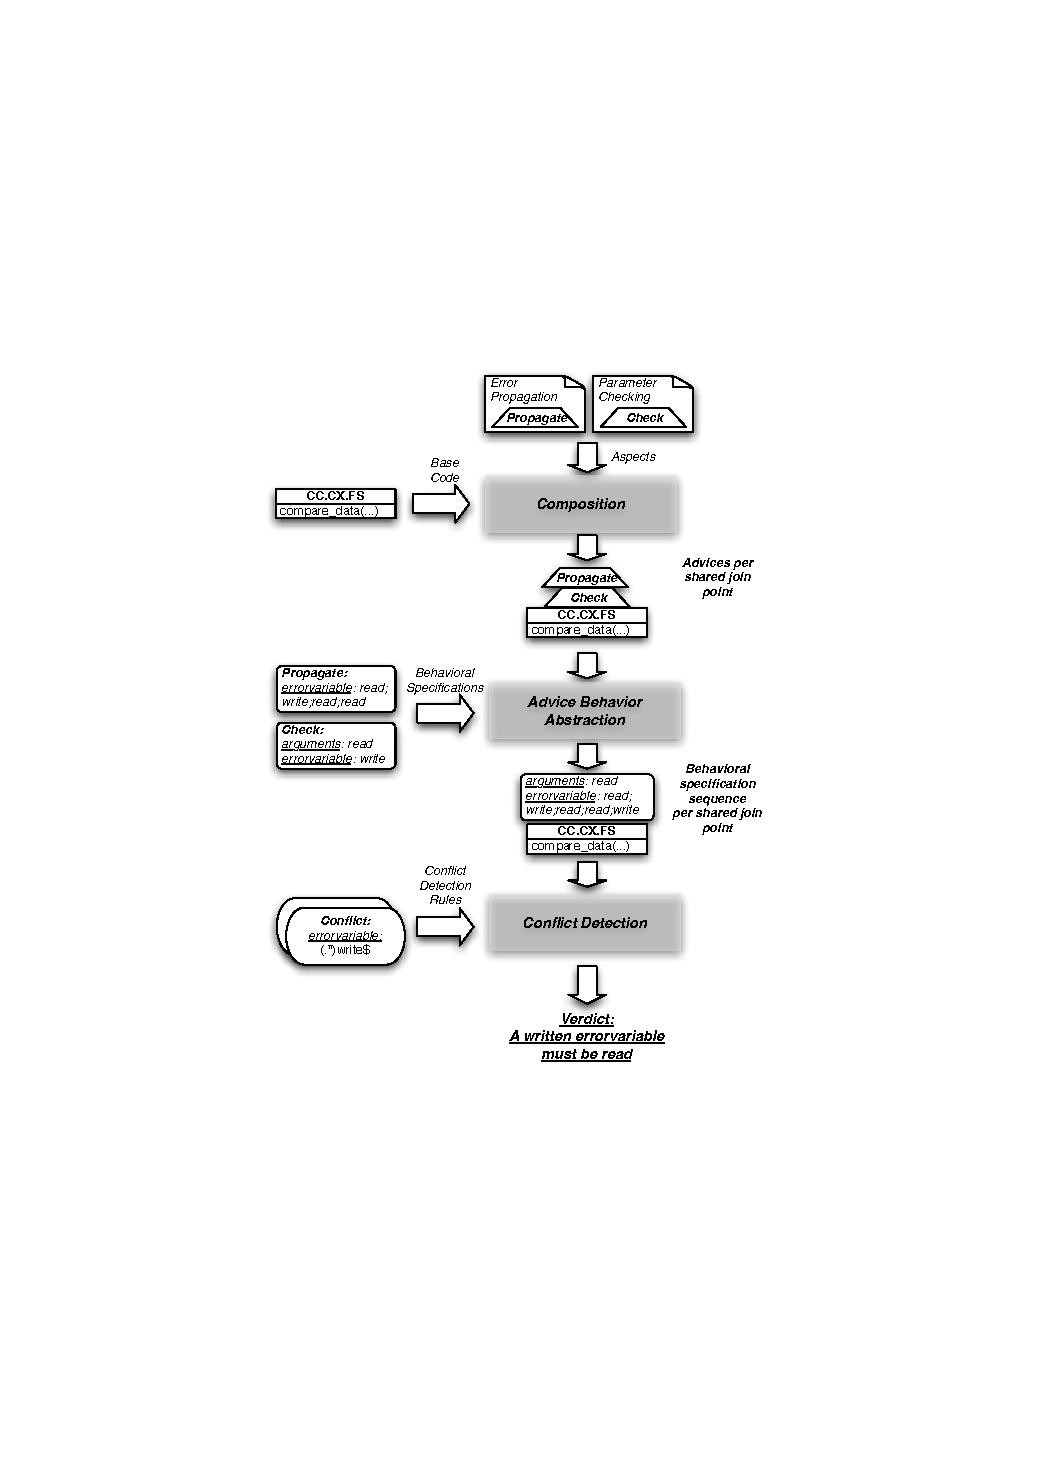
\includegraphics{./Figures/CompStages.pdf}
		\rule{35em}{0.5pt}
	\caption[Proceso de detecci�n de conflictos]{Proceso de detecci�n de conflictos.}
	\label{fig:Stages}
\end{figure}

 % Aspect-Oriented Programming

% Capitulo 4

\chapter{Aspect-Oriented Workflow Languages} % Write in your own chapter title
\label{Capitulo4}
\lhead{Capitulo 4. \emph{BPEL}} % Write in your own chapter title to set the page header

\section{Introducci�n}
�ste cap�tulo presenta las limitaciones de los lenguajes de \textit{workflow} con respecto a la modularidad de las preocupaciones transversales y la modularidad de los cambios. Dentro de las limitaciones de los sistemas de \textit{workflow} se encuentran la falta de soporte a los comportamientos transversales (\textit{crosscutting concerns}), es decir que los lenguajes no ofrecen elementos necesarios para implementar modularmente requerimientos que afectan transversalmente los procesos, tales como monitoreo de actividades, recolecci�n de datos, m�tricas, etc. Actualmente, para poder implementar estos cambios, es necesario modificar la especificaci�n del proceso, lo que tiene varias implicaciones negativas: 
\begin{itemize}
\item Las preocupaciones transversales pueden afectar m�s de un proceso, en m�s de un punto. Si el programador tiene que modificar la definici�n de los procesos para agregar �ste comportamiento, debe conocer todos los procesos y todos los lugares dentro de los procesos donde debe realizar la modificaci�n. �ste es un procedimiento largo, donde la probabilidad de inyectar errores es muy alta. 
\item Modificar la especificaci�n del proceso para satisfacer las preocupaciones transversales causa que  no exista una clara separaci�n entre los elementos que componen el proceso y los elementos que soportan los comportamientos transversales. 
\item Debido a que el comportamiento que satisface las preocupaciones transversales se encuentra dispersado a trav�s de los procesos, no hay manera de que los elementos que soportan los comportamientos transversales puedan ser activados o desactivados durante la ejecuci�n del proceso.
\item No poder expresar los cambios sobre una definici�n de procesos como entidades de primera clase implica que la �nica manera de poder conocer los cambios que ha sufrido un proceso, es comparando el proceso inicial con el actual para luego deducir los cambios.
\end{itemize}


\section{Problemas de Modularizaci�n de Lenguajes de Workflow}
Para poder ilustrar los problemas de moldularizaci�n de los lenguajes de \textit{workflow}, se establece el siguiente ejemplo de un proceso. 

\subsection{Ejemplo}
\label{sec:EjemploInterferencia}
En el mercado existen aplicaciones para dispositivos m�viles, mediante las cuales es posible identificar una canci�n, registrando a trav�s de un micr�fono un fragmento corto que est� sonando en la radio o en televisi�n. Una vez identificada la canci�n, es ofrecida al usuario para que la compre de diferentes tiendas de m�sica en l�nea. Ejemplos de �stas aplicaciones son Shazam\citep{Ref41} y Midomi\citep{Ref42}. 

En la figura \ref{fig:EjemploShazam} se muestra como puede ser el proceso de una de �stas aplicaciones. El proceso comienza cuando es recibida la informaci�n capturada a trav�s del micr�fono por la aplicaci�n. Una vez la solicitud es recibida, la siguiente actividad es encargada de comunicarse con el servicio que analiza la canci�n y como resultado provee la informaci�n completa de la canci�n. Al tener la informaci�n de la canci�n, dos actividades de b�squeda interact�an con dos tiendas de m�sica en l�nea, para buscar la informaci�n de compra para la canci�n. Luego la informaci�n es consolidada para posteriormente ser retornada al usuario.

\begin{figure}[htbp]
	\centering
		\includegraphics{./Figures/EjemploShazam.pdf}
		\rule{35em}{0.5pt}
	\caption[Ejemplo de un proceso workflow]{Ejemplo de un proceso workflow.}
	\label{fig:EjemploShazam}
\end{figure}

\subsection{Problemas de Modularizaci�n de Preocupaciones Transversales}
Para poder ilustrar como los lenguajes de \textit{workflow} no tienen los mecanismos necesarios de modularizaci�n para las preocupaciones transversales, se presentaran algunos ejemplos de recolecci�n de informaci�n y monitoreo de tiempo de ejecuci�n de actividades, basados en \citep{Ref40}.
\subsubsection{Recolecci�n de Informaci�n}
Pueden existir varios modelos de precios por usar los Web services de iTunes y de Amazon.com. Las pol�ticas de recaudaci�n pueden ser cobrar por cada llamado que se haga al Web service, cobrar a la empresa que haga m�s de cierto n�mero de consultas o cobrar por consultas que no resulten en una compra. En caso de existir dichas pol�ticas de cobro, el sistema debe poder llevar las cuentas de cuantos accesos a los Web services ha realizado el usuario, de �sta manera es posible corroborar que los cobros realizados por las tiendas de m�sica en l�nea es correcto. Para verificar la veracidad de una cuenta, el sistema debe contar cuantas veces el proceso ha ejecutado la actividad que se comunica con las tiendas de m�sica. 

Para poder implementar la funcionalidad de recolecci�n de informaci�n, se debe modificar todos los procesos de tal manera que cuando alguno de ellos se comunique con alguna de las tiendas de m�sica en l�nea se lleve la cuenta, c�mo lo muestra la figura \ref{fig:EjemploShazamContador}.
\begin{figure}[htbp]
	\centering
		\includegraphics{./Figures/EjemploShazamContador.pdf}
		\rule{35em}{0.5pt}
	\caption[Ejemplo de recolecci�n de informaci�n]{Ejemplo de recolecci�n de informaci�n.}
	\label{fig:EjemploShazamContador}
\end{figure}
Para poder implementar �ste cambio en BPEL, es necesario tener un Web service cuya funcionalidad es llevar la cuenta de los contadores. Se debe modificar la definici�n del proceso para agregar tanto las variables donde se va a llevar la cuenta, como los \textit{partner links} para poderse comunicar con el Web service anteriormente mencionado. Asimismo es necesario modificar la estructura del proceso para agregar un nuevo \textit{assign} antes de hacer el llamado a el Web Service que comunica el proceso con cada tienda de m�sica en l�nea, para poder establecer el valor del contador en la variable, para luego ser enviada a trav�s de un nuevo \textit{invoke} que llama el Web service para incrementar el contador.

La recolecci�n de datos es transversal, porque puede ocurrir en diferentes puntos del proceso, en diferentes procesos. La adici�n de la definici�n de las variables y de los \textit{partner links} tienen que repetirse en todos los procesos y tambi�n tiene que agregarse el \textit{assign} y el \textit{invoke} por cada ocurrencia de una actividad qu� se comunica con las tiendas de m�sica en l�nea, dispersando y repitiendo los mismos elementos muchas veces. Adem�s, no se va a tener una separaci�n clara entre cuales son los elementos del proceso y cu�les son los elementos usados para satisfacer las preocupaciones transversales.

\subsubsection{Monitoreo de Tiempo de Ejecuci�n de Actividades}
Las organizaciones que utilizan \textit{workflows} usualmente est�n interesadas en medir los tiempos de ejecuci�n de ciertas actividades de los procesos\citep{Ref40}. Si el sistema de \textit{workflow} que se utilice no provee las herramientas necesarias para poder realizar el monitoreo del tiempo de ejecuci�n de las actividades, una de las opciones es agregar �sta funcionalidad directamente sobre el proceso. Si se quiere agregar �sta funcionalidad a las dos actividades de b�squeda en el proceso de la figura \ref{fig:EjemploShazam}, obliga modificar el proceso para agregar una actividad cuando se quiere comenzar a monitorear el tiempo de ejecuci�n antes de la actividad a monitorear y agregar otra actividad despu�s, para detener el monitoreo, como lo muestra la figura \ref{fig:EjemploShazamTemporizador}.
\begin{figure}[htbp]
	\centering
		\includegraphics{./Figures/EjemploShazamTemporizador.pdf}
		\rule{35em}{0.5pt}
	\caption[Ejemplo monitoreo de tiempo de ejecuci�n]{Ejemplo monitoreo de tiempo de ejecuci�n.}
	\label{fig:EjemploShazamTemporizador}
\end{figure}
Una posible implementaci�n en BPEL, es crear un Web service de auditor�a e invocar operaciones para iniciar o parar un temporizador. Se debe modificar la definici�n del proceso para agregar tanto las variables donde se va a llevar la informaci�n de la actividad que est� siendo monitoreada, como los \textit{partner links} para poderse comunicar con el Web service anteriormente mencionado. Asimismo es necesario modificar la estructura del proceso para agregar un nuevo \textit{invoke} antes de la actividad que se quiere monitorear y un \textit{invoke} despu�s de la misma.

El monitoreo del tiempo de ejecuci�n de una actividad tambi�n es transversal, porque puede ocurrir en diferentes puntos del proceso, en diferentes procesos. La cantidad de elementos que se debe agregar es a�n mayor que en el ejemplo anterior.

\subsection{Problemas de Modularizaci�n de Cambios}
\label{sec:ProblemasModularizacion}
Para ilustrar las deficiencias que tienen los lenguajes de \textit{workflow} con respecto a la modularizaci�n de los cambios, se presentar�n algunos ejemplos de recolecci�n de informaci�n y monitoreo de tiempo de ejecuci�n de actividades, basados en \citep{Ref40}.

De acuerdo a \citep{Ref40} los cambios que puede sufrir una definici�n de un \textit{workflow} son los siguientes:
\begin{itemize}
\item \textbf{Cambios Evolutivos} - Los contextos donde se utilizan los sistemas de \textit{workflow} son altamente cambiantes. Multiples elementos pueden afectar en cualquier momento una definici�n de procesos, por ejemplo, nuevas estrategias de negocio, colaboraciones, nuevas condiciones externas, avance tecnol�gicos y cambios organizacionales. Estos cambios tienen que ser soportados  por los lenguajes de \textit{workflow}, ya que un cambio evolutivo va a afectar a todos los procesos junto con sus instancias.
\item \textbf{Cambios Ad-hoc} - Los cambios ad-hoc generalmente ocurren porque es imposible tener en cuenta todas las situaciones excepcionales al momento de dise�ar un proceso. Pueden ocurrir comportamientos inesperados debido a la interacci�n con usuarios, eventos impredecibles o situaciones err�neas. Los sistemas de \textit{workflow} deber�an proveer soporte para la adaptaci�n din�mica de las instancias de \textit{workflow}, para poder corregir dichas situaciones excepcionales.
\end{itemize}

Para poder ilustrar como los lenguajes de \textit{workflow} no tienen los mecanismos necesarios de modularizaci�n de cambios, se presentaran algunos ejemplos de incorporaci�n de un cambio evolutivo y un cambio ad-hoc, a partir del proceso mostrado en la figura \ref{fig:EjemploShazam}. Estos ejemplos son basados en \citep{Ref40}.
\subsubsection{Agregar una Actividad}
Se quiere modificar el proceso para que despu�s de buscar la canci�n en las tiendas de m�sica en l�nea, tenga una actividad extra que busque si el usuario es elegible para un c�digo de promoci�n, c�mo se muestra en la figura \ref{fig:EjemploShazamPromoCode}. 
\begin{figure}[htbp]
	\centering
		\includegraphics{./Figures/EjemploShazamPromoCode.pdf}
		\rule{35em}{0.5pt}
	\caption[Ejemplo agregar una actividad]{Ejemplo agregar una actividad.}
	\label{fig:EjemploShazamPromoCode}
\end{figure}

Para poder realizar �ste cambio, el programador tiene que bajar el proceso, modificarlo y luego volverlo a subir al servidor. En BPEL, se debe agregar un nuevo \textit{partner link} hacia el servicio que retorna un c�digo de promoci�n. Adem�s, debe agregar dos nuevas variables donde mantendr� la informaci�n de entrada y de salida para la actividad de b�squeda. En cuanto a la modificaci�n del control del proceso, es necesario agregar tres nuevas actividades. Primero, un \textit{assign} donde se establecer� el valor de la variable de entrada para la b�squeda del c�digo de promoci�n. Segundo, un \textit{invoke} que es qui�n llama al servicio de b�squeda. Tercero, otro \textit{assign} que copia la informaci�n de la b�squeda a la respuesta del proceso.

\section{AOP en Contextos Workflow}
\label{sec:AOPenWorkflow}
Gracias a que la orientaci�n por aspectos es una descomposici�n de uso general y paradigma de modularizaci�n, puede ser utilizado en otros contextos\citep{Ref40}. De la misma manera que AOP permite reducir la cantidad de c�digo enredado y repetido, y agregar nuevo comportamiento de manera modular en los lenguajes de programaci�n\citep{Ref27}, se ha propuesto aplicar est� t�cnica dentro de los contextos de programaci�n. 

Los lenguajes orientados por aspectos definen nuevos elementos al lenguaje que ser�n utilizados junto con los elementos del lenguaje existentes para proveer soporte a la modularidad, encapsulando los comportamientos transversales y los nuevos comportamientos. Estos elementos son:

\subsection{Modelo de \textit{Join Points}}
\label{sec:ModeloDeJoinPoints}
El modelo de \textit{join points} define los lugares donde los \textit{advices} van a ser ubicados en la ejecuci�n de la aplicaci�n base. Son puntos bien definidos, que proveen un marco de referencia com�n que hace posible que la ejecuci�n del c�digo del programa y la ejecuci�n del c�digo del \textit{advice} sea coordinada. 

De acuerdo a \citep{Ref40}, el modelo de \textit{join points} m�s intuitivo es basado en las actividades. La idea del modelo es que los \textit{join points} corresponden a las ejecuciones de las actividades y pueden ser diferenciados en dos:
\textbf{\textit{Join points} de Actividades} - Son \textit{joint points} de grano grueso, es decir, estos puntos capturan el inicio o la terminaci�n de la ejecuci�n de una actividad.
\textbf{\textit{Join points} Internos} - Son \textit{join points} de grano fino, capturan puntos internos en la ejecuci�n de una actividad. Estos son necesarios cuando los \textit{join points} de actividades no son lo suficientemente granulares para poder implementar alg�n comportamiento transversal.

\subsection{Lenguaje de Puntos de Corte}
El lenguaje de puntos de corte es utilizado para seleccionar un conjunto espec�fico de \textit{join points}. 

El lenguaje de puntos de corte, en contextos de \textit{workflows} puede ser pensado de dos maneras. La primera aproximaci�n es desarrollando un lenguaje de texto, como XML, donde mediante instrucciones espec�ficas o utilizando expresiones, se defina donde se quiere componer el nuevo comportamiento. La segunda es poder seleccionar sobre una representaci�n gr�fica del proceso, donde se quiere componer alg�n comportamiento nuevo. �sta aproximaci�n tiene la ventaja que la composici�n del nuevo comportamiento la puede hacer cualquier persona que est� familiarizada con el proceso, ya que se requerir�a una herramienta donde gr�ficamente se pueda seleccionar donde se quiere hacer la composici�n, para que despu�s la herramienta genere un archivo de texto o se comunique directamente con el servidor.

\subsection{Lenguaje de \textit{Advices}}
\label{section:WorkflowAdviceLanguages}
El lenguaje de \textit{advices} define la funcionalidad que debe ser ejecutada en los \textit{join points} espec�ficos. El \textit{advice} es un fragmento de c�digo que es ejecutado cuando se alcanza un \textit{join point} identificado por el respectivo punto de corte. El lenguaje de \textit{advices} generalmente es el mismo lenguaje que la aplicaci�n base. En lenguajes de \textit{workflow} orientados por aspectos el lenguaje de \textit{advices} deber�a ser el mismo que el lenguaje de \textit{workflow} base, para evitar equivocaciones de quien est� programando los \textit{advices}\citep{Ref43}. De acuerdo al modelo discutido en \ref{sec:ModeloAspectJ} los \textit{advices} pueden ser ejecutados antes, despu�s, o en vez de los \textit{join points} que son seleccionados por el punto de corte. 

\subsection{Tejido de Aspectos}
\label{section:WorkflowAspectWeaving}
El tejido de aspectos es la parte de la implementaci�n que debe asegurar que el c�digo de los \textit{advices} y �l de la aplicaci�n base se ejecuten de manera coordinada, en los \textit{join points} que fueron definidos para cada aspecto.

Existen dos maneras de hacer el tejido entre un proceso y sus aspectos\citep{Ref40}. De la primera forma, se conoce como tejido est�tico. Usando �sta manera de tejido, el proceso y los aspectos son tejidos antes de que se haga \textit{deploy} del proceso al motor. La otra forma se conoce como tejido din�mico y ocurre en ejecuci�n. Est�s dos aproximaciones implican dos maneras diferentes de implementar los motores donde se van a ejecutar tanto los procesos como los aspectos\citep{Ref40}.

\subsubsection{Transformaci�n de Procesos}
De �sta manera debe existir una herramienta de transformaci�n, que a partir de la definici�n del proceso y la definici�n de los aspectos, genere una nueva definici�n de proceso. �sta aproximaci�n soporta la composici�n est�tica, muy similar a como funciona AspectJ (secci�n \ref{sec:ModeloAspectJ}).

Una de las ventajas que tiene est� aproximaci�n es que cualquier motor de BPEL puede tomar la definici�n de proceso producida por la herramienta de transformaci�n y hacer \textit{deploy} del proceso sin modificar el motor. En cambio, la desventaja m�s clara, es que la composici�n no puede ser realizada en tiempo de ejecuci�n y por tanto, los aspectos no pueden tener puntos de corte que est�n relacionados con informaci�n que solo se tiene en ejecuci�n, a menos que se tengan en cuenta todas las posibilidades en dise�o. Adem�s, con �sta aproximaci�n, los aspectos no son definidos como entidades de primera clase, lo que implica que no se les puede hacer \textit{deploy} o \textit{undeploy} en tiempo de ejecuci�n.

\subsubsection{Modificaci�n del Motor para Verificaci�n de Aspectos}
En �sta aproximaci�n, el motor tiene que ser modificado para verificar s� debe realizar la ejecuci�n de un aspecto antes o despu�s de la ejecuci�n de cada actividad.

�sta aproximaci�n soporta la composici�n din�mica entre los aspectos y procesos. A diferencia de la aproximaci�n anterior, permite hacer \textit{deploy} y \textit{undeploy} de los aspectos, sin necesidad de crear nuevas instancias de procesos, lo cual es importante en caso de tener procesos que tardan mucho tiempo en ejecutar, ya que ser�a necesario detener la instancia, modificarla y tener pol�ticas para poder retornar la instancia al estado en el que se encontraba, como tambi�n pol�ticas para manejar las posibles inconsistencias. �sta aproximaci�n trata a los aspectos como entidades de primera clase, permitiendo que se puedan implementar funcionalidades de administraci�n en el motor. La desventaja de �sta aproximaci�n es que los archivos que componen a los aspectos est�n ligados a un solo motor.

\section{Lenguajes de BPEL Orientados Por Aspectos}
A continuaci�n se discuten dos de los lenguajes de BPEL orientados por aspectos m�s conocidos, utilizando los elementos descritos en la secci�n \ref{sec:AOPenWorkflow}.

\subsection{Padus}
\subsubsection{Modelo de \textit{Join Points}}

En Padus\citep{Ref43} el modelo de \textit{join points} est� relacionado con las actividades. Existen once tipos de \textit{join points} definidos para Padus, cada uno relacionado con una actividad BPEL especifica (ver tabla \ref{table:PadusJoinPoints}).

\begin{table}[htbp] 
\caption{Modelo de join points en Padus}  % title of Table 
\centering          % used for centering table 
\begin{tabular}{c}    % centered columns (4 columns) 
\hline\hline                        %inserts double horizontal lines 
Join Point \\ [0.5ex]  % inserts table 
%heading 
\hline                      % inserts single horizontal line 
		invoking \\ 
		receiving \\ 
		throwing \\ 
		compensating \\ 
		replying \\ 
		assigning \\ 
		terminating \\ 
		doingNothing (``empty") \\ 
		sequencing \\ 
		looping (``while") \\ 
		flowing \\ 
		switching \\ 
		picking \\ 
		scoping \\  [1ex]        % [1ex] adds vertical space 
\hline          %inserts single line 
\end{tabular} 
\label{table:PadusJoinPoints}% is used to refer this table in the text 
\end{table} 

\subsubsection{Lenguaje de Puntos de Corte}
El lenguaje de puntos de corte de Padus\citep{Ref43} est� compuesto por una serie de predicados que restringen los tipos de \textit{join points} (ver tabla \ref{table:PadusJoinPoints}) a partir de sus propiedades.  Los predicados definidos pueden ser combinados con predicados de Prolog, para as� poder restringir tambi�n sobre los tipos de datos, buscar en listas, etc. Como en los \textit{join points}, los predicados del lenguaje de puntos de corte, tambi�n permite definir o exponer propiedades de los \textit{join points}, para ser utilizadas en ejecuci�n.
\begin{table}[htbp] 
\caption{Modelo de puntos de corte en Padus}  % title of Table 
\centering          % used for centering table 
\begin{tabular}{p{8cm} p{6cm}}    % centered columns (4 columns) 
\hline\hline                        %inserts double horizontal lines 
Predicado & Descripci�n \\ [0.5ex]  % inserts table 
%heading 
\hline                      % inserts single horizontal line 
		invoking(Joinpoint, Name, PartnerLink, PortType, Operation, InputVariable, OutputVariable) & Todos los atributos posibles \\ 
		invoking(Joinpoint, Name, PartnerLink, PortType, Operation) & No importan los nombres de las variables de salida \\ 
		invoking(Joinpoint, PartnerLink, PortType, Operation) & Solo importan el partner link, el portType y operation \\ [1ex]        % [1ex] adds vertical space  
\hline          %inserts single line 
\end{tabular} 
\label{table:PadusPointCuts}% is used to refer this table in the text 
\end{table} 

\begin{lstlisting}[float, caption= Ejemplo de un punto de corte que identifica \textit{join points} que llaman una operaci�n cuyo nombre comienza con ``send"., label = code:PadusPointCut]
invoking(Joinpoint, 'smsService', 'smsServicePT', Operation),startsWith(Operation, 'send')
\end{lstlisting}

En el c�digo \ref{code:PadusPointCut} se muestra un ejemplo tomado de \citep{Ref43}, donde un punto de corte que identifica \textit{join points} que llaman una operaci�n cuyo nombre comienza con ``send".

\begin{lstlisting}[caption = Ejemplo de un punto de corte, label = code:PadusPointCut]
invoking(Joinpoint, 'smsService', 'smsServicePT', Operation),startsWith(Operation, 'send')
\end{lstlisting}


\subsubsection{Lenguaje de \textit{Advices}}
El lenguaje de los \textit{advices} en Padus\citep{Ref41} se define dentro de un elemento XML, utilizando los elementos definidos en BPEL. �ste lenguaje tambi�n permite definir \textit{advices} que pueden ser ejecutados antes, despu�s y en vez de la actividad que se haya seleccionado. Padus tambi�n introduce un concepto nuevo que es el \textit{in advice}. �ste tipo de \textit{in advice} permite agregar comportamiento extra dentro de una actividad, por ejemplo, agregando una nueva actividad dentro de un \textit{flow}.
\subsubsection{Tejido de Aspectos}
De los dos tipos de tejido, discutidos en la secci�n \ref{section:WorkflowAspectWeaving}, Padus hace el tejido de manera est�tica, es decir, hace una transformaci�n del proceso base y de los aspectos (figura \ref{fig:ArquPadus} tomada de \citep{Ref43}), para generar un proceso nuevo. La motivaci�n detr�s de usar esta aproximaci�n, es que Padus es utilizado en un contexto donde se espera que el motor se desempe�e con una alta eficiencia.

\begin{figure}[htbp]
	\centering
		\includegraphics{./Figures/ArquPadus.pdf}
		\rule{35em}{0.5pt}
	\caption[Arquitectura de Padus]{Arquitectura de Padus.}
	\label{fig:ArquPadus}
\end{figure}

\subsection{AO4BPEL}
\subsubsection{Modelo de \textit{Join Points}}
AO4BPEL soporta \textit{join points} de actividad y \textit{join points} internos\citep{Ref40} (secci�n \ref{sec:ModeloDeJoinPoints}). Los \textit{join points} internos pueden capturar puntos definidos dentro de las actividades, por ejemplo, justo antes de enviar un mensaje en un \textit{invoke}.

\subsubsection{Lenguaje de Puntos de Corte}
El lenguaje de puntos de corte en AO4BPEL\citep{Ref40} es XPath, debido a que es un leguaje basado en consultas, que provee mecanismos para que los puntos de corte no sean est�ticos y sean definibles por el usuario, adem�s de utilizar los atributos de los elementos BPEL para restringir mejor los \textit{join points} deseados. Gracias a que BPEL es un leguaje basado en XML, el uso de XPath es una decisi�n natural, porque permite seleccionar f�cilmente las actividades BPEL como puntos de corte.

Un ejemplo tomado de \citep{Ref40}, de un punto de corte que selecciona todas las actividades \textit{invoke}, cuyo nombre sea \textit{travelPackage} en cualquier proceso.

\begin{lstlisting}[caption= Ejemplo de un punto de corte en AO4BPEL., label = code:AO4BPELPointCut]
<pointcut>
//invoke[@operation="findAFlight"]
</pointcut>
\end{lstlisting}

Utilizado las ventajas de XPath, se pueden restringir los \textit{join points} de acuerdo a los atributos de los elementos, como lo muestra el siguiente ejemplo, donde se restringe que el \textit{join point} solo se aplicar� sobre la operaci�n \textit{findAFlight} del proceso llamado \textit{travelPackage}.
\begin{lstlisting}[caption= Ejemplo de un punto de corte en AO4BPEL., label = code:AO4BPELPointCutProcess]
<pointcut>
/process[@name="travelPackage"]//invoke[@operation="findAFlight"]
</pointcut>
\end{lstlisting}

\subsubsection{Lenguaje de \textit{Advices}}
El lenguaje de \textit{advices} que AO4BPEL utiliza es una versi�n modificada de BPEL\citep{Ref40}. El lenguaje provee elementos para que sea posible acceder al contexto de la instancia donde se est� ejecutando, es decir, ofrece elementos para acceder a valores de variables del \textit{join point} donde se encuentra, entre otras. El lenguaje de \textit{advices} tambi�n permite definir si el \textit{advice} se va a ejecutar antes, despu�s o en vez de una actividad o del envi� o recepci�n de un mensaje.

\subsubsection{Tejido de Aspectos}
Para el caso de AO4BPEL, el tejido se hace de manera din�mica, es decir, la implementaci�n del motor incluye verificaciones dentro del ciclo de vida de la actividad, para saber luego decidir si se debe ejecutar alg�n aspecto en el punto de corte que se est� ejecutando.

\subsubsection*{�D�nde se Hacen las Verificaciones?}
Para implementar AO4BPEL fue extendido BPWS4J, un motor de orquestaci�n producido por IBM. AO4BPEL modifica los estados del ciclo de vida de una actividad para incluir las verificaciones de si se debe ejecutar alg�n aspecto. 

\begin{figure}[htbp]
	\centering
		\includegraphics{./Figures/AO4BPELStates.pdf}
		\rule{35em}{0.5pt}
	\caption[Estados de una actividad de AO4BPEL]{Estados de una actividad de AO4BPEL.}
	\label{fig:AO4BPELStates}
\end{figure}

El ciclo de vida de una actividad se muestra en la figura \ref{fig:AO4BPELStates}\citep{Ref40}. Las verificaciones de los \textit{advices} son hechas dependiendo si el \textit{advice} es de tipo \textit{before}, \textit{after} o \textit{around} o si los \textit{advices} son de tipo interno. La verificaci�n para los \textit{advices} de tipo \textit{before} se hace cuando la actividad pasa de estado \textit{enabled} a estado \textit{running}. La verificaci�n para los \textit{advices} de tipo \textit{after} se hace cuando la actividad sale del estado \textit{complete}. Para los \textit{advices} internos, las verificaciones solo se hacen si la actividad es una actividad de interacci�n (secci�n \ref{sec:ActividadesInteraccion}) ya que el comportamiento se puede tejer antes, despu�s o en vez de recibir o mandar un mensaje. En �ste caso, las verificaciones se encuentran dentro del estado \textit{running}.

\subsubsection*{�Qu� se Verifica?}
Para cada uno de los posibles \textit{join points} es necesario verificar si existe un punto de corte asociado, a ese lugar en particular para la actividad que se est� ejecutando. En AO4BPEL el proceso comienza desde el momento que se hace \textit{deploy} de un aspecto. Al hacer \textit{deploy} del aspecto se eval�an las expresiones de los puntos de corte sobre los documentos XML de los aspectos, para obtener as� una serie de nodos XML para cada expresi�n de los puntos de corte, para luego poder extraer metainformaci�n, como nombres, tipos de actividad, etc, para ser guardada. Luego, al ejecutar una actividad, se compara la metainformaci�n de la actividad con la mentainformaci�n que fue previamente obtenida y en caso de concordar, quiere decir que ese punto de corte corresponde a esa actividad.

\subsubsection*{Ejecuci�n de los \textit{Advice}}
Para hablar acerca de c�mo AO4BPEL ejecuta los \textit{advices}, es necesario hablar acerca de su arquitectura.
\begin{figure}[htbp]
	\centering
		\includegraphics{./Figures/AO4BPELArq.pdf}
		\rule{35em}{0.5pt}
	\caption[Arquitectura del motor de AO4BPEL]{Arquitectura del motor de AO4BPEL.}
	\label{fig:AO4BPEArq}
\end{figure}
Al motor BPWS4J se le agregaron dos componentes, el \textit{aspect deployment tool} y el \textit{aspect runtime}.  \textit{\textbf{Aspect deployment tool}} es una aplicaci�n Web que permite hacer una administraci�n sencilla de los aspectos. A trav�s de �ste componente se puede hacer \textit{deploy} y \textit{undeploy} de los aspectos, junto con conocer cu�les son los aspectos que se encuentran en el servidor. El \textit{\textbf{Aspect runtime}} es responsable de manejar y ejecutar los aspectos. �ste componente es qui�n es responsable de realizar las verificaciones de los puntos de corte.
Debido a que el comportamiento est� definido en el \textit{advice} usando BPEL, el \textit{aspect runtime} delega la ejecuci�n de esa actividad al interpretador BPEL y coordina la ejecuci�n as�\citep{Ref40}:
\begin{itemize}
\item Si el tipo del \textit{advice} es \textit{before} o \textit{after} se suspende la ejecuci�n del proceso hasta que se complete la actividad del \textit{advice}, luego continua la ejecuci�n del proceso con la actividad suspendida.
\item Si el tipo del \textit{advice} es \textit{around} la ejecuci�n del proceso se suspende, luego, al terminar de ejecutar la actividad del \textit{advice}, la actividad suspendida salta el estado \textit{running}, terminando su ejecuci�n.
\end{itemize}

\section{Interferencia de Aspectos en Contextos Workflow}
A continuaci�n se presenta un ejemplo para ilustrar como los problemas de interferencia en aspectos, se presentan tambi�n en contextos de \textit{workflows}. Se agregar�n dos aspectos al ejemplo utilizado en la secci�n \ref{sec:EjemploInterferencia}.
\subsection{Facturaci�n por Busqueda}
\label{section:AspectoFacturacion}
Se quiere agregar la funcionalidad que se le cobre al usuario de la aplicaci�n por cada b�squeda que se realiza en las tiendas de m�sica en l�nea. Para implementar �ste cambio en las reglas de negocio se  implementa usando un aspecto. 

Una posible implementaci�n es tejer una actividad que env�e la informaci�n del usuario a un servicio de recaudo para que la consulta sea agregada a su cuenta como se muestra en la figura \ref{fig:AspectoFacturacion}. 

\begin{figure}[htbp]
	\centering
		\includegraphics{./Figures/Facturacion.pdf}
		\rule{35em}{0.5pt}
	\caption[Aspecto de facturaci�n]{Aspecto de facturaci�n.}
	\label{fig:AspectoFacturacion}
\end{figure}

\subsection{Cambios en las Pol�ticas de Distribuci�n}
Debido a que en Estados Unidos existe una ley llamada \textit{Digital Millennium Copyright Act (DMCA)}\citep{Ref44} el contenido que es distribuido fuera de Estados Unidos debe ser restringido. Es por �ste cambio en las reglas de negocio que se debe hacer una verificaci�n de la ubicaci�n donde se origin� la solicitud. Para implementar �ste cambio tambi�n se usa un aspecto.

Una posible implementaci�n es colocar un aspecto en vez (\textit{around}) de las actividades que buscan las canciones en las tiendas de m�sica en l�nea, de tal manera que se verifique la localizaci�n del usuario antes de buscar la canci�n y de ser una ubicaci�n no permitida, no hacer nada, como se muestra en la figura \ref{fig:AspectoUbicacion}

\begin{figure}[htbp]
	\centering
		\includegraphics{./Figures/AspectoUbicacion.pdf}
		\rule{35em}{0.5pt}
	\caption[Aspecto de verificaci�n de ubicaci�n]{Aspecto de verificaci�n de ubicaci�n.}
	\label{fig:AspectoUbicacion}
\end{figure}


\subsection{Interferencia Entre los Aspectos}

Para el caso de la composici�n de los dos aspectos anteriores en un \textit{join point} compartido, la interferencia se da porque es posible cobrarle a un usuario por una consulta que no se realiza.  Primero el proceso recibe la informaci�n del fragmento, junto con la ubicaci�n del usuario. Luego se llama la actividad que procesa el fragmento para obtener la informaci�n acerca de la canci�n. El siguiente paso es ejecutar el primer aspecto, invocando el servicio de recaudo para registrar el cobro del acceso al usuario. Luego, se procede a ejecutar el siguiente aspecto, el cual verifica la ubicaci�n del usuario y en el caso que no se encuentre en una ubicaci�n v�lida, no realiza la b�squeda en la tienda de m�sica en l�nea y no se tiene en cuenta el hecho que ya se le cobr� por esa consulta. S� el primer aspecto no fuera un aspecto de tipo antes sino de tipo despu�s, ocurrir�a lo mismo porque no se har�a el acceso hacia el servicio de b�squeda, pero se le terminar�a cobrando al usuario.  

Las pol�ticas de ordenamiento definidas por \textit{Padus} y por \textit{AO4BPEL} no funcionar�an, porque no es posible definir un orden donde se puedan ejecutar los aspectos sin que ocurra el problema de interferencia entre ellos. 



 % Aspect-Oriented Workflow Languages

% Capitulo 5

\chapter{El Proyecto Cumbia} % Write in your own chapter title
\label{Capitulo5}
\lhead{Capitulo 5. \emph{El Proyecto Cumbia}} % Write in your own chapter title to set the page header


Los sistemas de \textit{workflow} se desenvuelven en diferentes contextos (salud, educaci�n, negocios), debido a que cada contexto presenta necesidades diferentes, los sistemas de \textit{workflow} satisfacen de manera diferente esas necesidades. Sin embargo, todos tienen en com�n que los problemas se modelan ordenando y sincronizando la ejecuci�n de un conjunto de recursos o elementos para lograr un objetivo en un tiempo especifico. �stos se conocen como aplicaciones basadas en control. 

M�ltiples factores influencian tanto los contextos como las aplicaciones que las soportan y no es com�n que las arquitecturas de dichas aplicaciones no son lo suficientemente flexibles para poder adaptarse a estos cambios\citep{Ref45}.

El proyecto Cumbia\footnote{Proyecto Cumbia: \url{http://cumbia.uniandes.edu.co}} del grupo de construcci�n de software de la Universidad de los Andes. Es un proyecto de investigaci�n que propone la construcci�n  de f�bricas de software para la familia de aplicaciones basadas en control, donde predomine la evoluci�n y adaptaci�n de dichas aplicaciones. Una aplicaci�n Cumbia, es un conjunto de componentes que se comunican entre s� y uno de los  componentes tiene como responsabilidad manejar el control de la aplicaci�n\citep{Ref50}. 

Dentro de Cumbia, estos componentes se denominan activos. Estos activos est�n construidos a partir de modelos ejecutables. Los modelos ejecutables a su vez, est�n definidos por componentes modulares llamados objetos abiertos. Esta arquitectura permite tener un alto nivel de modularizaci�n, lo cual permite construir aplicaciones que cuentan con una arquitectura totalmente flexible, adem�s de exponer un modelo natural de composici�n de activos, no s�lo para definir nuevas aplicaciones sino tambi�n para generar activos reutilizables en la generaci�n de aplicaciones de la familia de control.\citep{Ref46}


\section{Aplicaciones Orientadas a Control}

El componente de control de una aplicaci�n est� compuesto por tres elementos principales. Primero, el conjunto de actividades que se deben ejecutar, segundo por el modelo de asignaci�n de responsables para estas actividades y tercero, por el orden en el cual se debe desarrollar su ejecuci�n. El componente de control es responsable de ordenar, administrar y sincronizar un conjunto de tareas de manera autom�tica para lograr un objetivo dado.\citep{Ref46}

Sin embargo, el componente de control no es el �nico componente que constituye sistemas complejos. Existen diferentes perspectivas pertenecientes a diferentes dominios, que tambi�n deben ser tenidas en cuenta y coordinadas para poder resolver el problema propuesto. Por ejemplo, el conjunto de responsables que se asignar�n a las tareas, ciertas restricciones de tiempo que puedan estar asociadas a la ejecuci�n de cada actividad y el uso de datos o recursos de contenido necesarios para el desarrollo de cada actividad son ejemplos de las preocupaciones que conforman un problema en donde el control es una necesidad principal.

El proyecto Cumbia propone una abstracci�n de metamodelos para poder modelar todas las perspectivas que hacen parte de un problema. Mediante el uso de los metamodelos, se describen todos los elementos de cada dominio particular y la construcci�n consecuente de modelos ejecutables conformes, que permitan la composici�n de las diferentes perspectivas para poder solucionar el problema.

\section{Metamodelos}

De acuerdo a \citep{Ref47} un modelo es la abstracci�n de un sistema construido para un prop�sito espec�fico. La especificaci�n de dicha abstracci�n se conoce como metamodelo. En un metamodelo se identifican los elementos relevantes y la relaci�n entre ellos. Gracias a los metamodelos es posible hacer una clara separaci�n de todas las perspectivas que componen un sistema complejo. �sta separaci�n permite la representaci�n de dominios que pueden ser comunes para diferentes aplicaciones y adem�s permite crear nuevas soluciones componiendo diferentes dominios.

En Cumbia, cada una de las perspectivas que hacen parte del problema se describen en un metamodelo. La definici�n de cada metamodelo est� compuesta por elementos de un dominio espec�fico que modifica o complementa el componente de control. Por ejemplo, asignaci�n de tiempo, manejo de recursos, manipulaci�n de datos, etc. A cada uno de los metamodelos se agrega sem�ntica de ejecuci�n materializando modelos conformes cuyos elementos se encuentran representados como objetos abiertos. 

Producto de la construcci�n de modelos conformes a cada uno de estos metamodelos, se obtiene un modelo ejecutable y extensible que cumple con dos caracter�sticas. Primero, ofrece elementos de composici�n en un nivel de granularidad muy fino, asegurando la flexibilidad del modelo. Segundo, garantiza la extensibilidad y adaptaci�n de los modelos a requerimientos cambiantes para los dominios que representan. La capacidad de composici�n y extensibilidad de estos modelos, ofrece ventajas relacionadas con modularidad y reutilizaci�n en la construcci�n de soluciones de manera flexible.\citep{Ref48}

\section{Modelo de Objetos Abiertos OO}
\label{section:OpenObjects}
Cumbia propone que los elementos que los elementos expresados en los metamodelos, sean implementados de tal manera que puedan exponer f�cilmente su sem�ntica de ejecuci�n. La propuesta es que se extienda el modelo tradicional de objetos, de tal manera que sea m�s f�cil componer y coordinar los elementos. 

Cada objeto abierto \ref{fig:opnObject} est� compuesto por un objeto tradicional llamado entidad, una maquina de estados, y un conjunto de acciones asociadas a las transiciones de los estados.
\begin{figure}[htbp]
	\centering
		\includegraphics{./Figures/opnObject.pdf}
		\rule{35em}{0.5pt}
	\caption[Estructura de un objeto abierto]{Estructura de un objeto abierto.}
	\label{fig:opnObject}
\end{figure}


Los objetos pueden tener muchos estados que son dependientes de los posibles valores que puedan tomar sus atributos en un momento dado, pero no todos los posibles estados son representativos o puedan interesarle a los dem�s objetos con los que interact�a. La m�quina de estados es utilizada para poder exponer los estados relevantes de la entidad a otros objetos. Ya que la m�quina de estados es la exposici�n del estado de la entidad, �sta siempre debe estar sincronizada con el estado interno de la entidad. El objeto interno sincroniza la m�quina de estados, movi�ndola de un estado a otro, de acuerdo a las acciones que se ejerzan sobre �l.

Al utilizar una m�quina de estados para exponer el estado de una entidad, es posible escuchar y/o generar eventos para mover otras m�quinas de estados. Cuando una maquina de estado escucha un evento, �ste es procesado y una transici�n es tomada para cambiar el estado actual, adem�s de sincronizar su estado interno de ser necesario. En las transiciones de los estados es posible definir acciones, que ser�n ejecutadas secuencialmente una vez la m�quina de estados cambie de un estado a otro a trav�s de esa transici�n. El uso de acciones permite generar nuevos eventos y de esta manera obtener coordinaci�n sincr�nica con otros objetos abiertos o componentes externos que pueda integrarse al sistema de eventos.\citep{Ref49}
 

\section{Modelos Ejecutables Cumbia}
Un modelo ejecutable representa la instancia de un metamodelo de dominio espec�fico, que gracias al uso de objetos abiertos, tiene sem�ntica de ejecuci�n y tambi�n permiten entretejerse a nivel de entidades o de m�quinas de estado con otros elementos definidos en el metamodelo.

\subsection{Estrategia de Composici�n de Modelos} 
\label{sec:composicion}
Una vez definidos tanto el modelo de control, como los dem�s modelos necesarios para obtener una aplicaci�n, se necesita un mecanismo que sea capaz de coordinar la interacci�n de los elementos de modelos heterog�neos. El mecanismo de entretejido propuesto, utiliza la misma estrategia de composici�n y coordinaci�n que se usa dentro de cada modelo: los objetos abiertos se coordinan a trav�s del paso de eventos, a�n si est�n definidos en dominios diferentes. Esta composici�n se realiza cuando los modelos se ejecutan, no existen tareas intermedias de compilaci�n\citep{Ref48}.

�sta estrategia de entretejido es an�loga a la utilizada en aspectos, el comportamiento de un modelo de control es enriquecido con otros modelos que representan las diferentes preocupaciones. Los \textit{join points} en �ste modelo est�n representados por los diferentes puntos alcanzables en las m�quinas de estado que se usan para coordinaci�n. Las ventajas de este tipo de construcciones son enumeradas en \citep{Ref48} como:
\begin{itemize}
\item El nivel de granularidad de los puntos de uni�n disponibles para la composici�n y coordinaci�n, es m�s alto que con otras aproximaciones. Estos puntos se encuentran m�s relacionados con el estado de los elementos y no con el flujo de control o las interfaces, por lo tanto pueden ser modificados de acuerdo con la aplicaci�n espec�fica que se est� construyendo.
\item �sta estrategia se puede aplicar en niveles complejos para entretejer preocupaciones sobre aplicaciones que ya contienen otros modelos entretejidos.
\item Cada preocupaci�n puede ser expresada de manera independiente usando lenguajes o metamodelos diferentes. Gracias a esto, se puede utilizar el metamodelo o mecanismo de extensi�n m�s adecuado para cada una de estas preocupaciones.
\end{itemize}

En la figura \ref{fig:comp} se muestra c�mo es posible crear aplicaciones separando los problemas de acuerdo a sus diferentes perspectivas y luego componi�ndolas gracias al uso de la materializaci�n de los modelos de cada dominio. En el ejemplo se muestra un modelo de control que especif�ca el orden y la sincronizaci�n del flujo de trabajo, un modelo de tiempo que permite definir reglas con diferentes patrones de tiempo, el dominio de roles que hace referencia a la estructura de usuarios en roles y los lugares donde ocurre la composici�n de los 3 modelos, en donde diferentes tareas tienen reglas de tiempo asociadas y son ejecutadas por un rol espec�fico. 
\begin{figure}[htbp]
	\centering
		\includegraphics{./Figures/application.pdf}
		\rule{35em}{0.5pt}
	\caption[Composici�n de Modelos de Diferentes Dominios]{Composici�n de Modelos de Diferentes Dominios.}
	\label{fig:comp}
\end{figure}
 % Cumbia

% Capitulo 6

\chapter{Caffeine v2.0: Motor BPEL sobre Cumbia} % Write in your own chapter title
\label{Capitulo6}
\lhead{Capitulo 6. \emph{Caffeine v2.0: Motor BPEL sobre Cumbia}} % Write in your own chapter title to set the page header


\section{Introducci�n}
Caffeine es un proyecto desarrollado dentro del marco de investigaci�n del proyecto Cumbia. La primera versi�n de este motor fue desarrollada por Daniel Romero como trabajo de tesis\citep{Ref51}. Con el objetivo de poder extender la funcionalidad del motor para hacerlo orientado por aspectos, fue necesario redise�arlo y reimplementarlo, es por eso que se desarrollo la versi�n 2.0.

\section{Elementos Presentes}
En el trabajo desarrollado en \citep{Ref51}, se propone una metodolog�a para construir motores de \textit{workflow} usando Cumbia. Dentro de la metodolog�a se propone que los elementos del lenguaje deben ser agrupados por capas, de tal manera que sea posible hacer un desarrollo incremental del motor de \textit{workflow} que se busca construir\citep{Ref51}. All� mismo se hizo una divisi�n de los elementos BPEL en tres capas. La primera capa se coloc� todos los elementos de BPEL que se consideran necesarios para poder definir un proceso de forma completa (sin manejo de fallas ni funcionalidad adicional). En la segunda capa, se clasificaron los elementos asociados con el manejo de fallas y transacciones. En la tercera capa se encuentran los elementos que permiten extender el lenguaje, definiendo elementos personalizables. Los elementos desarrollados en la segunda versi�n de Caffeine son los elementos que se muestran en la tabla \ref{table:ElementosCapa1}.

\begin{table}[htbp] 
\caption{Elementos de la Capa 1}  % title of Table 
\centering          % used for centering table 
\begin{tabular}{ p{3cm} p{8cm}}    % centered columns (4 columns) 
\hline\hline                        %inserts double horizontal lines 
Elemento & Descripci�n\\ [0.5ex]  % inserts table 
%heading 
\hline                      % inserts single horizontal line 
process & Elemento ra�z. \\      % inserting body of the table 
partnerLink & Describe un servicio colaborador, incluyendo roles (de cada parte involucrada) y la operaci�n a ser invocada (WSDL portType). \\ 
variables & Elemento para declarar un conjunto de variables.  \\ 
variable & Dato usado en el proceso. \\ 
receive & Bloqueo para esperar de un mensaje proveniente de uno de los partnerLink del proceso.   \\ 
reply & Respuesta enviada a uno de los partnerLink.   \\ 
invoke & Invoca uno de los servicios colaboradores, bien sea de forma as�ncrona o sincr�nica.  \\ 
assign (copy, query, from, to, literal, expression) & Permite copiar datos en las variables.  \\ 
wait (until, for) & Suspende la operaci�n por un per�odo dado de tiempo.  \\ 
empty & No hacer nada. \\ 
sequence & Ejecuta una serie de actividades en orden secuencial.  \\ 
flow & Ejecuci�n de actividades de forma paralela. \\ 
if, elseIf, else (condition) & Instrucci�n condicional. \\ 
while & Instrucci�n repetitiva.\\ 
pick & Bloquearse y esperar por un mensaje o alarma. \\ 
onMessage & Elemento definido dentro de pick o eventHandler. Bloquearse y esperar por un mensaje. \\ 
onAlarm & Elemento definido dentro de pick y eventHandler. Bloquearse y esperar a que un periodo de tiempo se cumpla. \\ 
exit & Termina y destruye los procesos de forma inmediata. \\ [1ex]        % [1ex] adds vertical space 
\hline          %inserts single line 
\end{tabular} 
\label{table:ElementosCapa1}    % is used to refer this table in the text 
\end{table}

Debido a la cantidad de elementos, se decidi� dividirlos en categor�as para mejor ilustraci�n.

\subsection{Elementos de Inicio}
Un proceso BPEL no se inicia cuando el usuario lo indica. Para poder iniciar un proceso BPEL se deben definir elementos para que al recibir un mensaje se instancie el proceso\citep{Ref6}, esos elementos se encuentran agrupados en �sta categor�a. 

\begin{figure}[htbp]
	\centering
		\includegraphics{./Figures/startingPoint.pdf}
		\rule{35em}{0.5pt}
	\caption[Elementos de inicio]{Elementos de inicio.}
	\label{fig:ElementosInicio}
\end{figure}

\subsubsection{Elemento \textit{Process}}
\label{section:ElementProcess}
�ste elemento es el encargado de agrupar todas las actividades para alcanzar un objetivo.
\begin{figure}[htbp]
	\centering
		\includegraphics{./Figures/process.pdf}
		\rule{35em}{0.5pt}
	\caption[M�quina de estados del elemento \textit{Process}]{M�quina de estados del elemento \textit{Process}.}
	\label{fig:ProcessStateMachine}
\end{figure}

\begin{table}[htbp] 
\caption{Estados del Elemento \textit{Process}}  % title of Table 
\centering          % used for centering table 
\begin{tabular}{p{0.2\textwidth}|p{0.75\textwidth}}
	\multicolumn{2}{l}{\textbf{\large{Descripci�n de Estados}}} \\ \hline\hline	
	Init &  Es el estado inicial del elemento.\\ \hline
	Waiting & Una vez el elemento es inicializado, queda en espera hasta que se reciba el mensaje que indica que va a comenzar su ejecuci�n. Este estado tambi�n es utilizado para indicar que el proceso est� detenido, debido a que alguna actividad interna bloquea el proceso.\\ \hline
	ExecutingActivity &  Este estado indica que se encuentra ejecutando una actividad interna.\\ \hline
	Finalizing &  En este estado se indica que la ejecuci�n del elemento ya termin�.\\ \hline
	\hline
\end{tabular}
\label{table:EstadosProcess}    % is used to refer this table in the text 
\end{table}

\begin{table}[htbp] 
\caption{Acciones del elemento \textit{Process}}  % title of Table 
\centering          % used for centering table 
\begin{tabular}{p{0.3\textwidth}|p{0.65\textwidth}}
	\multicolumn{2}{l}{\textbf{\large{Acciones}}} \\ \hline\hline	
	InitActivities &  Realiza todas las actividades necesarias para inicializar las actividades internas del proceso.\\ \hline
	Execute &  Ejecuta la primera actividad definida para el proceso.\\ \hline
	ExecuteNext &  Ejecuta la siguiente actividad en el proceso.\\ \hline
	\hline
\end{tabular}
\label{table:AccionesProcess}    % is used to refer this table in the text 
\end{table}




\subsubsection{Elemento \textit{StartingPick}}
El elemento \textit{StartingPick} representa cuando un \textit{Pick} es configurado para que cuando llegue un mensaje inicie la ejecuci�n del proceso. 
\begin{figure}[htbp]
	\centering
		\includegraphics{./Figures/startingPick.pdf}
		\rule{35em}{0.5pt}
	\caption[M�quina de estados del elemento \textit{StartingPick}]{M�quina de estados del elemento \textit{StartingPick}.}
	\label{fig:StartingPickStateMachine}
\end{figure}
\begin{table}[htbp] 
\caption{Estados del Elemento \textit{StartingPick}}  % title of Table 
\centering          % used for centering table 
\begin{tabular}{p{0.2\textwidth}|p{0.75\textwidth}}
	\multicolumn{2}{l}{\textbf{\large{Descripci�n de Estados}}} \\ \hline\hline	
	Init &  Es el estado inicial del proceso.\\ \hline
	Waiting & Una vez el elemento es inicializado, queda en espera hasta que se reciba el mensaje que indica que va a comenzar su ejecuci�n. Este estado tambi�n es utilizado para indicar que el proceso est� detenido, debido a que alguna actividad interna bloquea el proceso.\\ \hline
	Executing &  Este estado indica que se encuentra ejecutando la actividad asociada al elemento.\\ \hline
	Finalizing &  En este estado se indica que la ejecuci�n del elemento ya termin�.\\ \hline
	\hline
\end{tabular}
\label{table:EstadosStartingReceive}    % is used to refer this table in the text 
\end{table}

\begin{table}[htbp] 
\caption{Acciones del elemento \textit{StartingPick}}  % title of Table 
\centering          % used for centering table 
\begin{tabular}{p{0.3\textwidth}|p{0.65\textwidth}}
	\multicolumn{2}{l}{\textbf{\large{Acciones}}} \\ \hline\hline	
	RegisterReceive &  Registra al elemento como un elemento que est� esperando un mensaje.\\ \hline
	RegisterOnMessage &  Ejecuta la actividad asociada al elemento.\\ \hline

	\hline
\end{tabular}
\label{table:AccionesStartingPick}    % is used to refer this table in the text 
\end{table}



\subsubsection{Elemento \textit{StartingReceive}}
El elemento \textit{StartingReceive} representa cuando un \textit{Receive} es configurado para que cuando llegue un mensaje inicie la ejecuci�n del proceso. 
\begin{figure}[htbp]
	\centering
		\includegraphics{./Figures/startingReceive.pdf}
		\rule{35em}{0.5pt}
	\caption[M�quina de estados del elemento \textit{StartingReceive}]{M�quina de estados del elemento \textit{StartingReceive}.}
	\label{fig:StartingReceiveStateMachine}
\end{figure}

\begin{table}[htbp] 
\caption{Estados del Elemento \textit{StartingReceive}}  % title of Table 
\centering          % used for centering table 
\begin{tabular}{p{0.2\textwidth}|p{0.75\textwidth}}
	\multicolumn{2}{l}{\textbf{\large{Descripci�n de Estados}}} \\ \hline\hline	
	Init &  Es el estado inicial de la actividad.\\ \hline
	Waiting & Una vez el elemento es inicializado, queda en espera hasta que se reciba el mensaje que indica que va a comenzar su ejecuci�n.\\ \hline
	Finalizing &  En este estado se indica que la ejecuci�n del elemento ya termin�.\\ \hline
	\hline
\end{tabular}
\label{table:EstadosStartingReceive}    % is used to refer this table in the text 
\end{table}
\begin{table}[htbp] 
\caption{Acciones del elemento \textit{StartingReceive}}  % title of Table 
\centering          % used for centering table 
\begin{tabular}{p{0.3\textwidth}|p{0.65\textwidth}}
	\multicolumn{2}{l}{\textbf{\large{Acciones}}} \\ \hline\hline	
	RegisterReceive &  Registra al elemento como un elemento que est� esperando un mensaje.\\ \hline
	\hline
\end{tabular}
\label{table:AccionesStartingReceive}    % is used to refer this table in the text 
\end{table}



\subsection{Elementos de Interacci�n}
Los elementos de interacci�n son aquellos que pueden enviar o recibir mensajes de los colaboradores y realizar una acci�n conforme.
\begin{figure}[htbp]
	\centering
		\includegraphics{./Figures/interaction.pdf}
		\rule{35em}{0.5pt}
	\caption[Elementos de interacci�n]{Elementos de interacci�n.}
	\label{fig:ElementosInteraccion}
\end{figure}


\subsubsection{Elemento \textit{Pick}}
El elemento \textit{Pick} espera la ocurrencia de exactamente un evento de un conjunto de eventos, luego ejecuta la actividad asociada con ese evento. Despu�s que se ha seleccionado un evento, los dem�s eventos no son aceptados\citep{Ref6}.
\begin{figure}[htbp]
	\centering
		\includegraphics{./Figures/pick.pdf}
		\rule{35em}{0.5pt}
	\caption[M�quina de estados del elemento \textit{Pick}]{M�quina de estados del elemento \textit{Pick}.}
	\label{fig:PickStateMachine}
\end{figure}

\begin{table}[htbp] 
\caption{Estados del Elemento \textit{Pick}}  % title of Table 
\centering          % used for centering table 
\begin{tabular}{p{0.2\textwidth}|p{0.75\textwidth}}
	\multicolumn{2}{l}{\textbf{\large{Descripci�n de Estados}}} \\ \hline\hline	
	Init &  Es el estado inicial del elemento.\\ \hline
	Waiting & Una vez el elemento es inicializado, queda en espera hasta que se dispare el temporizador de alguno de sus \textit{onAlarm} o alguno de sus \textit{onMessage} reciba un mensaje. \\ \hline
	Executing &  Una vez seleccionada la actividad, pasa a ejecutarla. Este estado indica que se encuentra ejecutando dicha actividad.\\ \hline
	Finalizing &  En este estado se indica que la ejecuci�n del elemento ya termin�.\\ \hline
	\hline
\end{tabular}
\label{table:EstadosPick}    % is used to refer this table in the text 
\end{table}

\begin{table}[htbp] 
\caption{Acciones del elemento \textit{Pick}}  % title of Table 
\centering          % used for centering table 
\begin{tabular}{p{0.3\textwidth}|p{0.65\textwidth}}
	\multicolumn{2}{l}{\textbf{\large{Acciones}}} \\ \hline\hline	
	InitElements &  Realiza todas las actividades necesarias para inicializar los \textit{onAlarm} y \textit{onMessage} asociados al elemento.\\ \hline
	Execute &  Ejecuta la actividad que fue seleccionada.\\ \hline
	\hline
\end{tabular}
\label{table:AccionesProcess}    % is used to refer this table in the text 
\end{table}




\subsubsection{Elemento \textit{OnAlarm}}
 El elemento \textit{onAlarm} corresponde a un temporizador, que tiene una actividad asociada. Cuando el temporizador se termina, se lo informa al \textit{Pick} al que pertenece, para que este tome la decisi�n si se debe ejecutar o no  la actividad.
\begin{figure}[htbp]
	\centering
		\includegraphics{./Figures/onAlarm.pdf}
		\rule{35em}{0.5pt}
	\caption[M�quina de estados del elemento \textit{OnAlarm}]{M�quina de estados del elemento \textit{onAlarm}.}
	\label{fig:onAlarmStateMachine}
\end{figure}

\begin{table}[htbp] 
\caption{Estados del Elemento \textit{onAlarm}}  % title of Table 
\centering          % used for centering table 
\begin{tabular}{p{0.2\textwidth}|p{0.75\textwidth}}
	\multicolumn{2}{l}{\textbf{\large{Descripci�n de Estados}}} \\ \hline\hline	
	Init &  Es el estado inicial del elemento.\\ \hline
	Counting & Indica que el temporizador del elemento se encuentra activo.\\ \hline
	Finalizing &  En este estado se indica que la ejecuci�n del elemento ya termin�, debido a que el temporizador termino.\\ \hline
	\hline
\end{tabular}
\label{table:EstadosOnAlarm}    % is used to refer this table in the text 
\end{table}

\begin{table}[htbp] 
\caption{Acciones del elemento \textit{onAlarm}}
\centering          % used for centering table 
\begin{tabular}{p{0.3\textwidth}|p{0.65\textwidth}}
	\multicolumn{2}{l}{\textbf{\large{Acciones}}} \\ \hline\hline	
	StartCounter &  Inicia el temporizador del elemento.\\ \hline
	SetActivityOnPick &  Le indica al \textit{Pick} al que pertenece, que termino el temporizador y le pasa la actividad. Es responsabilidad del \textit{Pick} decidir si esa es la actividad que se debe ejecutar.\\ \hline
	\hline
\end{tabular}
\label{table:AccionesOnAlarm}    % is used to refer this table in the text 
\end{table}



\subsubsection{Elemento \textit{OnMessage}}
El elemento \textit{onMessage} espera hasta recibir un mensaje de un colaborador.
\begin{figure}[htbp]
	\centering
		\includegraphics{./Figures/onMessage.pdf}
		\rule{35em}{0.5pt}
	\caption[M�quina de estados del elemento \textit{onMessage}]{M�quina de estados del elemento \textit{onMessage}.}
	\label{fig:onMessageStateMachine}
\end{figure}

\begin{table}[htbp] 
\caption{Estados del Elemento \textit{onMessage}}  % title of Table 
\centering          % used for centering table 
\begin{tabular}{p{0.2\textwidth}|p{0.75\textwidth}}
	\multicolumn{2}{l}{\textbf{\large{Descripci�n de Estados}}} \\ \hline\hline	
	Init &  Es el estado inicial del elemento.\\ \hline
	Waiting & Una vez el elemento es inicializado, queda en espera hasta que se reciba un mensaje.\\ \hline
	Finalizing &  En este estado se indica que la ejecuci�n del elemento ya termin�.\\ \hline
	\hline
\end{tabular}
\label{table:EstadosOnMessage}    % is used to refer this table in the text 
\end{table}

\begin{table}[htbp] 
\caption{Acciones del elemento \textit{onMessage}}  % title of Table 
\centering          % used for centering table 
\begin{tabular}{p{0.3\textwidth}|p{0.65\textwidth}}
	\multicolumn{2}{l}{\textbf{\large{Acciones}}} \\ \hline\hline	
	RegisterOnMessage &  Ejecuta la actividad asociada al elemento.\\ \hline
	SetActivityOnPick &  Le indica al \textit{Pick} al que pertenece, que recibo un mensaje y le pasa la actividad. Es responsabilidad del \textit{Pick} decidir si esa es la actividad que se debe ejecutar.\\	\hline
\end{tabular}
\label{table:AccionesOnMessage}    % is used to refer this table in the text 
\end{table}



\subsubsection{Elemento \textit{Receive}}
El elemento \textit{Receive} es el encargado de recibir mensajes de los colaboradores.
\begin{figure}[htbp]
	\centering
		\includegraphics{./Figures/receive.pdf}
		\rule{35em}{0.5pt}
	\caption[M�quina de estados del elemento \textit{Receive}]{M�quina de estados del elemento \textit{Receive}.}
	\label{fig:ReceiveStateMachine}
\end{figure}

\begin{table}[htbp] 
\caption{Estados del Elemento \textit{Receive}}  % title of Table 
\centering          % used for centering table 
\begin{tabular}{p{0.2\textwidth}|p{0.75\textwidth}}
	\multicolumn{2}{l}{\textbf{\large{Descripci�n de Estados}}} \\ \hline\hline	
	Init &  Es el estado inicial del elemento.\\ \hline
	Waiting & Una vez el elemento es inicializado, queda en espera hasta que se reciba un mensaje.\\ \hline
	Finalizing &  En este estado se indica que la ejecuci�n del elemento ya termin�.\\ \hline
	\hline
\end{tabular}
\label{table:EstadosReceive}    % is used to refer this table in the text 
\end{table}

\begin{table}[htbp] 
\caption{Acciones del elemento \textit{Receive}}  % title of Table 
\centering          % used for centering table 
\begin{tabular}{p{0.3\textwidth}|p{0.65\textwidth}}
	\multicolumn{2}{l}{\textbf{\large{Acciones}}} \\ \hline\hline	
	RegisterOnMessage &  Ejecuta la actividad asociada al elemento.\\ \hline
	\hline
\end{tabular}
\label{table:AccionesReceive}    % is used to refer this table in the text 
\end{table}


\subsubsection{Elemento \textit{Reply}}
El elemento \textit{Reply} es utilizado para enviar una respuesta a una solicitud previamente aceptada, a trav�s de un elemento de interacci�n.
\begin{figure}[htbp]
	\centering
		\includegraphics{./Figures/reply.pdf}
		\rule{35em}{0.5pt}
	\caption[M�quina de estados del elemento \textit{Reply}]{M�quina de estados del elemento \textit{Reply}.}
	\label{fig:ReplyStateMachine}
\end{figure}

\begin{table}[htbp] 
\caption{Estados del Elemento \textit{Reply}}  % title of Table 
\centering          % used for centering table 
\begin{tabular}{p{0.2\textwidth}|p{0.75\textwidth}}
	\multicolumn{2}{l}{\textbf{\large{Descripci�n de Estados}}} \\ \hline\hline	
	Init &  Es el estado inicial del elemento.\\ \hline
	Finalizing &  En este estado se indica que la ejecuci�n del elemento ya termin�.\\ \hline
	\hline
\end{tabular}
\label{table:EstadosReply}    % is used to refer this table in the text 
\end{table}

\begin{table}[htbp] 
\caption{Acciones del elemento \textit{Reply}}  % title of Table 
\centering          % used for centering table 
\begin{tabular}{p{0.3\textwidth}|p{0.65\textwidth}}
	\multicolumn{2}{l}{\textbf{\large{Acciones}}} \\ \hline\hline	
	SendMessage &  Env�a el mensaje.\\ \hline
	\hline
\end{tabular}
\label{table:AccionesReply}    % is used to refer this table in the text 
\end{table}



\subsubsection{Elemento \textit{Invoke}}
El elemento \textit{Invoke}  es utilizado para enviar mensajes a los colaboradores. �ste elemento puede ser configurado para en env�e el mensaje y termine o para que env�e el mensaje y quede esperando una respuesta.
\begin{figure}[htbp]
	\centering
		\includegraphics{./Figures/invoke.pdf}
		\rule{35em}{0.5pt}
	\caption[M�quina de estados del elemento \textit{Invoke}]{M�quina de estados del elemento \textit{Invoke}.}
	\label{fig:InvokeStateMachine}
\end{figure}

\begin{table}[htbp] 
\caption{Estados del Elemento \textit{Invoke}}  % title of Table 
\centering          % used for centering table 
\begin{tabular}{p{0.2\textwidth}|p{0.75\textwidth}}
	\multicolumn{2}{l}{\textbf{\large{Descripci�n de Estados}}} \\ \hline\hline	
	Init &  Es el estado inicial del elemento.\\ \hline
	MessageSent & Indica que env�o el mensaje al colaborador.\\ \hline
	Waiting &  Este estado solo es alcanzado si el elemento tiene que esperar una respuesta del colaborador.\\ \hline
	Finalizing &  En este estado se indica que la ejecuci�n del elemento ya termin�.\\ \hline
	\hline
\end{tabular}
\label{table:EstadosInvoke}    % is used to refer this table in the text 
\end{table}

\begin{table}[htbp] 
\caption{Acciones del elemento \textit{Invoke}}  % title of Table 
\centering          % used for centering table 
\begin{tabular}{p{0.3\textwidth}|p{0.65\textwidth}}
	\multicolumn{2}{l}{\textbf{\large{Acciones}}} \\ \hline\hline	
	SendMessage &  Env�a el mensaje al colaborador.\\ \hline
	RegisterReceive &  Registra que es una actividad que est� esperando la llegada de un mensaje.\\ \hline
	\hline
\end{tabular}
\label{table:AccionesInvoke}    % is used to refer this table in the text 
\end{table}


\subsection{Elementos Estructuradores}
Los elementos estructuradores son los que forman el proceso, influenciando en que orden se van a ejecutar los elementos que se encuentran dentro de ellos. 
\begin{figure}[htbp]
	\centering
		\includegraphics{./Figures/interaction.pdf}
		\rule{35em}{0.5pt}
	\caption[Elementos estructuradores]{Elementos estructuradores.}
	\label{fig:ElementosEstructuradores}
\end{figure}


\subsubsection{Elemento \textit{Sequence}}
�ste elemento contiene una o m�s actividades que son ejecutadas en serie.
\begin{figure}[htbp]
	\centering
		\includegraphics{./Figures/sequence.pdf}
		\rule{35em}{0.5pt}
	\caption[M�quina de estados del elemento \textit{Sequence}]{M�quina de estados del elemento \textit{Sequence}.}
	\label{fig:SequencetateMachine}
\end{figure}

\begin{table}[htbp] 
\caption{Estados del Elemento \textit{Sequence}}  % title of Table 
\centering          % used for centering table 
\begin{tabular}{p{0.2\textwidth}|p{0.75\textwidth}}
	\multicolumn{2}{l}{\textbf{\large{Descripci�n de Estados}}} \\ \hline\hline	
	Init &  Es el estado inicial del elemento.\\ \hline
	Executing &  Este estado indica que se encuentra ejecutando una actividad interna.\\ \hline
	Waiting & Debido a que la ejecuci�n de un elemento puede bloquear el proceso, el elemento \textit{Sequence} se bloquea hasta que la actividad en ejecuci�n tambi�n se desbloquee.\\ \hline
	Finalizing &  En este estado se indica que la ejecuci�n del elemento ya termin�.\\ \hline
	\hline
\end{tabular}
\label{table:EstadosSequence}    % is used to refer this table in the text 
\end{table}

\begin{table}[htbp] 
\caption{Acciones del elemento \textit{Sequence}}  % title of Table 
\centering          % used for centering table 
\begin{tabular}{p{0.3\textwidth}|p{0.65\textwidth}}
	\multicolumn{2}{l}{\textbf{\large{Acciones}}} \\ \hline\hline	
	ExecuteFirst &  Ejecuta la primera actividad de la secuencia.\\ \hline
	ExecuteNext &  Ejecuta la siguiente actividad, de no haber siguiente le indica al elemento que termin�.\\ \hline
	\hline
\end{tabular}
\label{table:AccionesSequence}    % is used to refer this table in the text 
\end{table}



\subsubsection{Elemento \textit{Flow}}
El elemento \textit{Flow} contiene una o m�s actividades que son ejecutadas en paralelo.
\begin{figure}[htbp]
	\centering
		\includegraphics{./Figures/flow.pdf}
		\rule{35em}{0.5pt}
	\caption[M�quina de estados del elemento \textit{Flow}]{M�quina de estados del elemento \textit{Flow}.}
	\label{fig:FlowStateMachine}
\end{figure}

\begin{table}[htbp] 
\caption{Estados del Elemento \textit{Flow}}  % title of Table 
\centering          % used for centering table 
\begin{tabular}{p{0.2\textwidth}|p{0.75\textwidth}}
	\multicolumn{2}{l}{\textbf{\large{Descripci�n de Estados}}} \\ \hline\hline	
	Init &  Es el estado inicial del elemento.\\ \hline
	Executing &  Este estado indica que se encuentra ejecutando alguna de las actividades internas.\\ \hline
	Waiting & Debido a que la ejecuci�n de un elemento puede bloquear el proceso, el elemento \textit{Flow} debe esperar hasta que todas las actividades internas se desbloqueen.\\ \hline
	Finalizing &  En este estado se indica que la ejecuci�n del elemento ya termin�.\\ \hline
	\hline
\end{tabular}
\label{table:EstadosFlow}    % is used to refer this table in the text 
\end{table}

\begin{table}[htbp] 
\caption{Acciones del elemento \textit{Flow}}  % title of Table 
\centering          % used for centering table 
\begin{tabular}{p{0.3\textwidth}|p{0.65\textwidth}}
	\multicolumn{2}{l}{\textbf{\large{Acciones}}} \\ \hline\hline	
	ExecuteAll &  Ejecuta todas las actividades que contiene.\\ \hline
	CheckAllTerminated &  Verifica que todas las actividades hayan terminado su ejecuci�n.\\ \hline
	AddWaiting &  Agrega a un contador que una actividad est� esperando.\\ \hline
	SubtractWaiting &  Resta del contador una actividad que dejo de esperar.\\ \hline
	\hline
\end{tabular}
\label{table:AccionesFlow}    % is used to refer this table in the text 
\end{table}



\subsubsection{Elemento \textit{While}}
�ste elemento provee una ejecuci�n repetida para el elemento que contiene.
\begin{figure}[htbp]
	\centering
		\includegraphics{./Figures/while.pdf}
		\rule{35em}{0.5pt}
	\caption[M�quina de estados del elemento \textit{While}]{M�quina de estados del elemento \textit{While}.}
	\label{fig:WhileStateMachine}
\end{figure}

\begin{table}[htbp] 
\caption{Estados del Elemento \textit{While}}  % title of Table 
\centering          % used for centering table 
\begin{tabular}{p{0.2\textwidth}|p{0.75\textwidth}}
	\multicolumn{2}{l}{\textbf{\large{Descripci�n de Estados}}} \\ \hline\hline	
	Init &  Es el estado inicial del elemento.\\ \hline
	Evaluating &  Indica que se encuentra evaluando la condici�n de repetici�n del \textit{While}.\\ \hline
	Executing&  Una vez evaluada la condici�n como cierta, debe pasar a ejecutar el elemento. Este estado indica que se encuentra ejecutando la actividad interna.\\ \hline
	Waiting & El elemento interno puede pasar a un estado de espera, lo que bloquea el elemento \textit{While} hasta que la actividad interna se desbloquee.\\ \hline
	Finalizing &  En este estado se indica que la ejecuci�n del elemento ya termin�.\\ \hline
	\hline
\end{tabular}
\label{table:EstadosWhile}    % is used to refer this table in the text 
\end{table}

\begin{table}[htbp] 
\caption{Acciones del elemento \textit{While}}  % title of Table 
\centering          % used for centering table 
\begin{tabular}{p{0.3\textwidth}|p{0.65\textwidth}}
	\multicolumn{2}{l}{\textbf{\large{Acciones}}} \\ \hline\hline	
	Evaluate &  Eval�a la condici�n de repetici�n del elemento.\\ \hline
	Execute &  Ejecuta el elemento interno.\\ \hline
	\hline
\end{tabular}
\label{table:AccionesWhile}    % is used to refer this table in the text 
\end{table}




\subsubsection{Elemento \textit{Condicional}}
BPEL no tiene un elemento llamado "`condicional"', pero provee elementos como \textit{If, ElseIf, Else} para proveer este comportamiento. Se decidi� encapsular a los tres elementos dentro de una actividad \textit{Condicional}  para poder exponer el estado de la ejecuci�n de los tres elementos, en uno solo.
\begin{figure}[htbp]
	\centering
		\includegraphics{./Figures/conditional.pdf}
		\rule{35em}{0.5pt}
	\caption[M�quina de estados del comportamiento \textit{Condicional}]{M�quina de estados del elemento \textit{Condicional}.}
	\label{fig:CondicionalStateMachine}
\end{figure}

\begin{table}[htbp] 
\caption{Estados del Elemento \textit{Condicional}}  % title of Table 
\centering          % used for centering table 
\begin{tabular}{p{0.2\textwidth}|p{0.75\textwidth}}
	\multicolumn{2}{l}{\textbf{\large{Descripci�n de Estados}}} \\ \hline\hline	
	Init &  Es el estado inicial del elemento.\\ \hline
	If & Indica que el elemento est� realizando la evaluaci�n de la condici�n que se encuentra definida para el \textit{If}.\\ \hline
	ElseIf&  Indica que la evaluaci�n del elemento \textit{If} fue negativa, y que est� realizando la evaluaci�n de la condici�n que se encuentra definida para cada uno de los \textit{ElseIf}.\\ \hline
	Else &  Indica que la evaluaci�n de todas las condiciones de los elementos \textit{ElseIf} fue negativa, resultando en la ejecuci�n de la condici�n por defecto o en la ejecuci�n de nada.\\ \hline
	Executing &  Indica que encontr� una condici�n verdadera y que est� ejecutando la actividad del elemento correspondiente.\\ \hline
	Waiting & Si la actividad en ejecuci�n debe bloquearse, el elemento tiene que esperar hasta que la actividad contin�e con su ejecuci�n.\\ \hline
	Finalizing &  En este estado se indica que la ejecuci�n del elemento ya termin�.\\ \hline
	\hline
\end{tabular}
\label{table:EstadosCondicional}    % is used to refer this table in the text 
\end{table}

\begin{table}[htbp] 
\caption{Acciones del elemento \textit{Condicional}}  % title of Table 
\centering          % used for centering table 
\begin{tabular}{p{0.3\textwidth}|p{0.65\textwidth}}
	\multicolumn{2}{l}{\textbf{\large{Acciones}}} \\ \hline\hline	
	EvaluateIf &  Evalua la condici�n del elemento \textit{If}, en caso de ser verdadera ejecuta la actividad all� definida, de lo contrario comienza a evaluar los \textit{ElseIf}.\\ \hline
	ExecuteIf &  Ejecuta la actividad definida para el elemento \textit{If}.\\ \hline
	EvaluateElseIf &  Evalua la condici�n de los elementos \textit{ElseIf}, en caso de encontrar uno que sea verdadera, ejecuta su actividad asociada.\\ \hline
	ExecuteElseIf &  Ejecuta la actividad asociada con el elemento \textit{ElseIf}.\\ \hline
	ExecuteElse &  Ejecuta la actividad asociada al elemento \textit{Else}.\\ \hline
	\hline
\end{tabular}
\label{table:AccionesCondicional}    % is used to refer this table in the text 
\end{table}

\subsection{Instrucciones}
\begin{figure}[htbp]
	\centering
		\includegraphics{./Figures/instructions.pdf}
		\rule{35em}{0.5pt}
	\caption[Instrucciones]{Instrucciones.}
	\label{fig:ElementosEstructuradores}
\end{figure}



\subsubsection{Elemento \textit{Exit}}
�ste elemento es utilizado para terminar de ejecutar la instancia del proceso.
\begin{figure}[htbp]
	\centering
		\includegraphics{./Figures/exit.pdf}
		\rule{35em}{0.5pt}
	\caption[M�quina de estados del elemento \textit{Exit}]{M�quina de estados del elemento \textit{Exit}.}
	\label{fig:ExitStateMachine}
\end{figure}

\begin{table}[htbp] 
\caption{Estados del Elemento \textit{Exit}}  % title of Table 
\centering          % used for centering table 
\begin{tabular}{p{0.2\textwidth}|p{0.75\textwidth}}
	\multicolumn{2}{l}{\textbf{\large{Descripci�n de Estados}}} \\ \hline\hline	
	Init &  Es el estado inicial del elemento.\\ \hline
	Finalizing &  En este estado se indica que la ejecuci�n del elemento ya termin�.\\ \hline
	\hline
\end{tabular}
\label{table:EstadosExit}    % is used to refer this table in the text 
\end{table}

\begin{table}[htbp] 
\caption{Acciones del elemento \textit{Exit}}  % title of Table 
\centering          % used for centering table 
\begin{tabular}{p{0.3\textwidth}|p{0.65\textwidth}}
	\multicolumn{2}{l}{\textbf{\large{Acciones}}} \\ \hline\hline	
	ExitProcess &  Realiza todas las actividades necesarias para terminar la ejecuci�n de la instancia del proceso.\\ \hline
	\hline
\end{tabular}
\label{table:AccionesExit}    % is used to refer this table in the text 
\end{table}




\subsubsection{Elemento \textit{Empty}}
Este es un elemento que representa una actividad que no hace nada.
\begin{figure}[htbp]
	\centering
		\includegraphics{./Figures/empty.pdf}
		\rule{35em}{0.5pt}
	\caption[M�quina de estados del elemento \textit{Empty}]{M�quina de estados del elemento \textit{Empty}.}
	\label{fig:EmptyStateMachine}
\end{figure}

\begin{table}[htbp] 
\caption{Estados del Elemento \textit{Empty}}  % title of Table 
\centering          % used for centering table 
\begin{tabular}{p{0.2\textwidth}|p{0.75\textwidth}}
	\multicolumn{2}{l}{\textbf{\large{Descripci�n de Estados}}} \\ \hline\hline	
	Init &  Es el estado inicial del elemento.\\ \hline
	Finalizing &  En este estado se indica que la ejecuci�n del elemento ya termin�.\\ \hline
	\hline
\end{tabular}
\label{table:EstadosEmpty}    % is used to refer this table in the text 
\end{table}



\subsubsection{Elemento \textit{Wait}}
�ste elemento especifica una espera de un tiempo determinado o hasta que determinado plazo sea alcanzado.
\begin{figure}[htbp]
	\centering
		\includegraphics{./Figures/wait.pdf}
		\rule{35em}{0.5pt}
	\caption[M�quina de estados del elemento \textit{Wait}]{M�quina de estados del elemento \textit{Wait}.}
	\label{fig:WaitStateMachine}
\end{figure}

\begin{table}[htbp] 
\caption{Estados del Elemento \textit{Wait}}  % title of Table 
\centering          % used for centering table 
\begin{tabular}{p{0.2\textwidth}|p{0.75\textwidth}}
	\multicolumn{2}{l}{\textbf{\large{Descripci�n de Estados}}} \\ \hline\hline	
	Init &  Es el estado inicial del elemento.\\ \hline
	Waiting & Indica que la actividad se encuentra esperando que se venza el plazo determinado se termine un temporizador.\\ \hline
	Finalizing &  En este estado se indica que la ejecuci�n del elemento ya termin�.\\ \hline
	\hline
\end{tabular}
\label{table:EstadosWait}    % is used to refer this table in the text 
\end{table}

\begin{table}[htbp] 
\caption{Acciones del elemento \textit{Wait}}  % title of Table 
\centering          % used for centering table 
\begin{tabular}{p{0.3\textwidth}|p{0.65\textwidth}}
	\multicolumn{2}{l}{\textbf{\large{Acciones}}} \\ \hline\hline	
	StartingWait &  Inicia el temporizador.\\ \hline
	\hline
\end{tabular}
\label{table:AccionesWait}    % is used to refer this table in the text 
\end{table}


\subsubsection{Elemento \textit{Assign}}
�ste elemento es utilizado para copiar datos de una variable a otra o para insertar nuevos valores.
\begin{figure}[htbp]
	\centering
		\includegraphics{./Figures/assign.pdf}
		\rule{35em}{0.5pt}
	\caption[M�quina de estados del elemento \textit{Assign}]{M�quina de estados del elemento \textit{Assign}.}
	\label{fig:AssignStateMachine}
\end{figure}

\begin{table}[htbp] 
\caption{Estados del Elemento \textit{Assign}}  % title of Table 
\centering          % used for centering table 
\begin{tabular}{p{0.2\textwidth}|p{0.75\textwidth}}
	\multicolumn{2}{l}{\textbf{\large{Descripci�n de Estados}}} \\ \hline\hline	
	Init &  Es el estado inicial del elemento.\\ \hline
	Copying & Indica que se est� copiando los valores de una variable a otra.\\ \hline
	Finalizing &  En este estado se indica que la ejecuci�n del elemento ya termin�.\\ \hline
	\hline
\end{tabular}
\label{table:EstadosAssign}    % is used to refer this table in the text 
\end{table}

\begin{table}[htbp] 
\caption{Acciones del elemento \textit{Assign}}  % title of Table 
\centering          % used for centering table 
\begin{tabular}{p{0.3\textwidth}|p{0.65\textwidth}}
	\multicolumn{2}{l}{\textbf{\large{Acciones}}} \\ \hline\hline	
	ExecuteFirstCopy &  Realiza la copia del primer elemento interno.\\ \hline
	ExecuteNext &  Realiza la copia del siguiente elemento si existe.\\ \hline
	\hline
\end{tabular}
\label{table:AccionesAssign}    % is used to refer this table in the text 
\end{table}


\section{Arquitectura}

En �sta secci�n se hablar� de la arquitectura de Caffeine.

\begin{figure}[htbp]
	\centering
		\includegraphics{./Figures/Caffeine.pdf}
		\rule{35em}{0.5pt}
	\caption[Arquitectura de Caffeine]{Arquitectura de Caffeine.}
	\label{fig:CaffeineArq}
\end{figure}

\subsection{CumbiaOpenObjectsKernel}
\label{section:CumbiaOpenObjectsKernel}
El trabajo con metamodelos ejecutables extensibles ha sido un trabajo constante en el proyecto Cumbia. A partir de la tesis de maestria de Pablo Barvo y Mario S�nchez\citep{Ref52} se desarroll� un \textit{framework} para la f�cil generaci�n de otras aplicaciones y f�cil definici�n de nuevos metamodelos ejecutables usando objetos abiertos. 
A continuaci�n se describe a grandes rasgos cuales son las responsabilidades de �ste \textit{framework} y a describir algunos de sus elementos. �ste componente fue desarrollado por Mario S�nchez, uno de los integrantes del Proyecto Cumbia como parte de su trabajo doctoral. 

La responsabilidad principal de �ste \textit{Kernel}, es la de a partir de una serie de archivos que definen el metamodelo, crear e instanciar sus modelos, siendo sus elementos objetos abiertos o elementos que puedan generar o esperar eventos. Adem�s, es el responsable de realizar la coordinaci�n de todas las m�quinas de estado de los objetos.

El primer archivo que debe crearse para poder utilizar el  \textit{framework} es un XML (c�digo \ref{listing:BPELMetamodel}) donde se definen cuales son los elementos que componen el metamodelo. De igual manera en este archivo se indica cu�l es el archivo que define la m�quina de estados para cada elemento.
\begin{lstlisting}[language=xml,float, escapechar=\%, caption= Archivo de declaraci�n de los elementos del metamodelo., label=listing:BPELMetamodel ]
<metamodel name="BPEL" version="0.1">
	
	<!-- State machines used by the elments of the metamodel -->
	<state-machine-reference name="assign" file="assign.xml" />
	...
	<state-machine-reference name="while" file="while.xml" />	
	
	<!-- Elements of the metamodel -->
	<type name="Assign" class="uniandes.cumbia.bpel.elements.assign.Assign" statemachine="assign"/>
	...
	<type name="Copy" class="uniandes.cumbia.bpel.elements.assign.copy.Copy"/>
	...
	<type name="From" class="uniandes.cumbia.bpel.elements.assign.from.From"/>
	
	...
</metamodel>
\end{lstlisting}

Lugo de tener la definici�n de los elementos que componen el metamodelo, se debe implementar para cada metamodelo definido una serie de activos que permitan construir e instanciar el modelo con la estructura especifica, de tal manera el \textit{Kernel} sabe como cargar de un archivo la estructura del modelo. Adem�s de saber c�mo cargar la estructura del modelo, debe saber cu�l es el modelo que debe crear, �ste se define en un archivo archivo que contiene espec�ficamente cuales son los elementos que componen un modelo en particular (c�digo \ref{listing:ModelXML}). Por �ltimo, se debe crear la implementaci�n de todos los elementos que hacen parte del modelo y asociarlos al \textit{Kernel}.

\begin{lstlisting}[language=xml,float, escapechar=\%, caption= Archivo de definici�n de los elementos del metamodelo., label=listing:ModelXML]
<?xml version="1.0" encoding="UTF-8"?>
<definition metamodel="BPEL" modelName="HelloWorld" version="0.1">
		<metamodel-extensions/>
		<elements>
			<open-object name="HelloWorld" typeName="Process"/>
			...
			<open-object name="replyOutput" typeName="Reply"/>
		</elements>
		<runtime/>
		<model>
			<process ...>
			         
			    <!-- List of services participating in this BPEL process -->    
			    <partnerLinks>
			    ...
			    </partnerLinks>
			  
			    <!-- List of messages and XML documents used as part of this BPEL process -->    
			    <variables>
			    ...
			    </variables>
			
			    <!-- Orchestration Logic -->
			    <sequence name="sequence">
					...			        
			    </sequence>
			</process>
		</model>
</definition>
\end{lstlisting}






\subsection{CaffeineEngine}
�ste es el componente principal de Caffeine. �ste es el motor encargado de hacer \textit{deploy} de las definiciones de los procesos, crear las nuevas instancias de los procesos y el encargado de hacer la coordinaci�n del intercambio de mensajes.

\begin{figure}[htbp]
	\centering
		\includegraphics{./Figures/CaffeineEngine.pdf}
		\rule{35em}{0.5pt}
	\caption[Arquitectura de CaffeineEngine]{Arquitectura de CaffeineEngine.}
	\label{fig:CaffeineEngineArq}
\end{figure}

\subsubsection*{\textit{Process Space}}
El \textit{Process Space} es encargado de mantener las definiciones de proceso y crear las instancias de los procesos cuando sea necesario. Por cada proceso existente en el motor hay un correspondiente textit{Process Space}. 
\subsubsection*{\textit{Instance Space}}
El \textit{Instance Space} es quien contiene al elemento ra�z del proceso (\textit{Process}\label{section:ElementProcess}). De igual manera contiene una serie de elementos que monitorean la ejecuci�n de elementos para prop�sitos administrativos.
\subsubsection*{\textit{Message Center}}
Este componente es el encargado de la administraci�n de los mensajes recibidos o enviados por los colaboradores.  Cuando recibe un mensaje, se encarga de localizar la instancia a la cual le pertenece y entreg�rsela al elemento que le corresponde. De igual manera mantiene una lista de todos los colaboradores que hacen parte de los procesos, para que los procesos puedan enviar los mensajes a los colaboradores.

\subsubsection*{Protocolo de Instanciaci�n de un Proceso}
Este protocolo describe la manera como se realiza la creaci�n de una nueva instancia de proceso cuando se recibe un mensaje que no est� dirigido a una instancia existente. 

\textbf{1} - El Web service que representa el proceso recibe un mensaje dirigido a alguno de los elementos de inicio del proceso.

\textbf{2} - El \textit{MessageCenter} es encargado de revisar que el mensaje no est� dirigido a una instancia existente del proceso.

\textbf{3} - Al no existir una instancia a la cual pertenezca el mensaje, el \textit{MessageCenter} crea una instancia nueva del proceso.

\textbf{4} - Luego el mensaje es transmitido a la actividad de inicio a la cual es dirigido.

\textbf{5} - La actividad de inicio procesa el mensaje y le indica al proceso que debe comenzar su ejecuci�n.

\subsubsection*{Protocolo de Env�o de un Mensaje a un Colaborador}
A continuaci�n se presenta los pasos para realizar la invocaci�n de un Web service. 
\textbf{1} - Durante la ejecuci�n de una instancia, una actividad \textit{Invoke} le indica al motor que va a invocar un servicio (proporcionando la informaci�n de �ste) y el mensaje a ser enviado.

\textbf{2} - El motor, utilizando el Web service que representa el proceso, solicita la invocaci�n del \textit{partnerLink} especificado al \textit{MessageCenter}. 

\subsubsection*{Protocolo de Recepci�n de Mensaje por una Instancia Existente}
Este protocolo describe la manera como se realiza la creaci�n de una nueva instancia de proceso cuando se recibe un mensaje que est� dirigido a una instancia existente. 

\textbf{1} - Durante la ejecuci�n de una instancia de proceso, una actividad \textit{receive} pide al motor que la registre como una actividad que est� esperando un mensaje.
 
\textbf{2} - Cuando un mensaje llega, el \textit{MessageCenter} verifica entre los elementos que se registraron para esperar un mensaje.

\textbf{3} - Al encontrar el elemento al cual le pertenece el mensaje recibido, se lo notifica

\textbf{4} - Al entregar el mensaje, la actividad se elimina de la lista de actividades que est�n esperando mensaje.


\subsection{CaffeineDeployer}
La responsabilidad de este componente es la de traducir el archivo BPEL de entrada al archivo que recibe el \textit{framework} de objetos abiertos y de generar los archivos requeridos para publicar el proceso como un Web service.

\begin{figure}[htbp]
	\centering
		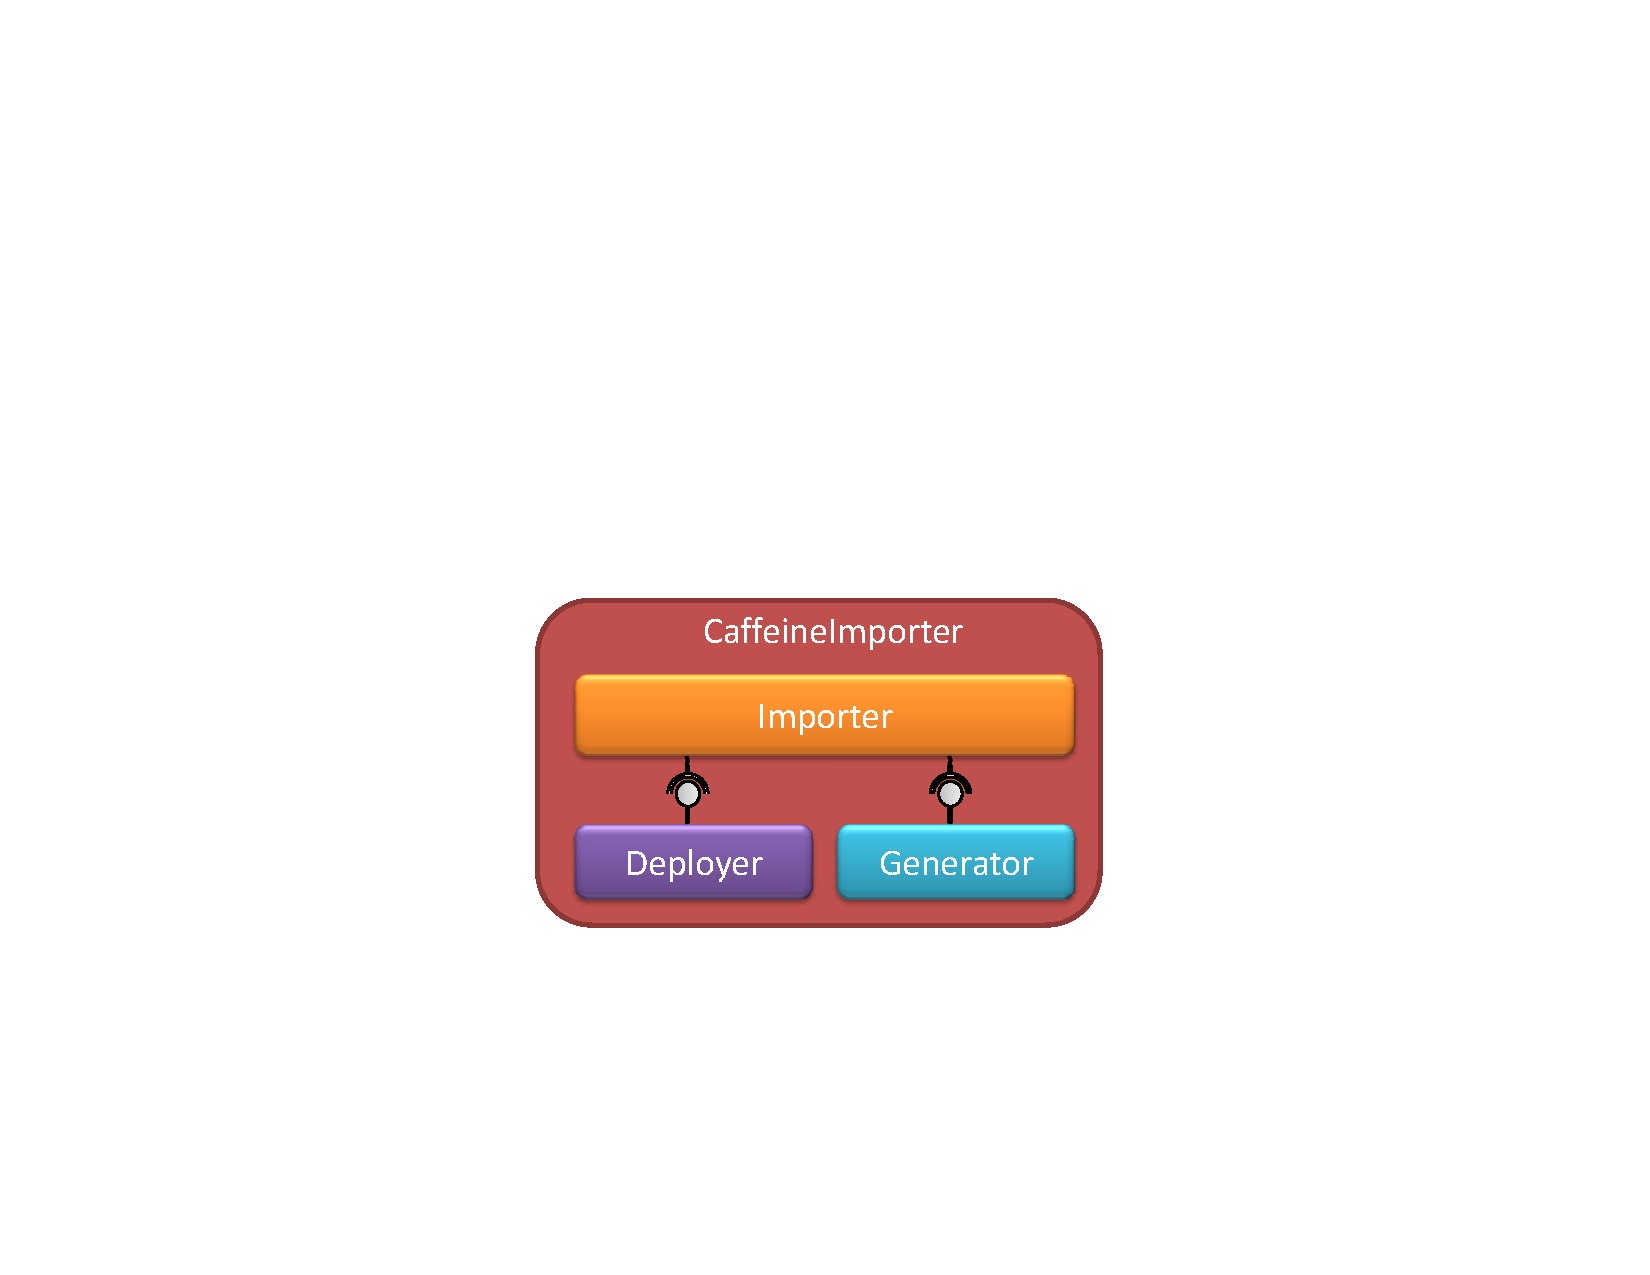
\includegraphics{./Figures/CaffeineImporter.pdf}
		\rule{35em}{0.5pt}
	\caption[Arquitectura del CaffeineDeployer]{Arquitectura de CaffeineDeployer.}
	\label{fig:CaffeineImporterArq}
\end{figure}

\subsubsection*{\textit{Importer}}
El \textit{Importer} es el componente principal del \textit{CaffeineDeployer}. �ste es el encargado de leer un archivo con un proceso BPEL y crear una serie de objetos que representan el proceso, pero estos objetos no tienen ning�n tipo de l�gica, son creados para mantener la informaci�n que est� contenida en los nodos XML. 

\subsubsection*{\textit{Generator}}
Parte del \textit{Generator} son una serie de \textit{visitors} que recorren la estructura de los elementos que representan el proceso y generan el archivo del modelo discutido en la secci�n \ref{section:CumbiaOpenObjectsKernel}. El \textit{Generator} permite la generaci�n de las clases para definir un Web service a partir del archivo WSDL del proceso BPEL.

\subsubsection*{\textit{Deployer}}
El Deployer tambi�n es el encargado de publicar los procesos BPEL, una vez finalice la importaci�n, para que puedan ser utilizados como Web services.


\section{Pruebas}

Para probar la correcta implementaci�n de \textit{Caffeine} se utiliz� otro de los activos del proyecto Cumbia, el \textit{CumbiaTestFramework}, el cual fue desarrollado como tesis de grado\citep{Ref49} por Sergio Moreno.

\subsection{Framework de Pruebas}
El \textit{framework} de pruebas provee un mecanismo para poder hacer pruebas sobre aplicaciones basadas en objetos abiertos. La idea principal del \textit{framework} de pruebas es poder monitorear el comportamiento de un motor sin interferir con su ejecuci�n, lo que presenta una serie de retos debido a que es necesario monitorear todos los elementos que pertenecen a un proceso, sus eventos, maquinas de estado, etc. 

Para hacer esto, el \textit{framework} est� dividido en un modelo de capas, que representan las diferentes etapas por las cuales puede pasar un proceso. 
La primera capa es la capa que tiene el metamodelo que se quiere probar. La segunda capa es la encargada de materializar los modelos que se van a probar. La tercera capa es la encargada de crear la instancia del motor que se quiere probar, crear la instancia del proceso que se quiere probar. En la cuarta capa  est�n definidos dos elementos b�sicos: sensores y trazas. Los sensores son elementos que se colocan sobre los elementos que se quiere monitorear, de esta manera es posible conocer, por ejemplo, los eventos que han sido generados desde cierto elemento o los estados de una m�quina que se activaron. Cuando un sensor es activado por alguno de los elementos que est� monitoreando, esa informaci�n es guardada en una traza, de tal manera teniendo un registro de que sensores fueron activados por cuales elementos y porque raz�n. Por �ltimo existe la capa de prueba, �sta capa es la encarga de realizar aserciones sobre las trazas que fueron creadas durante la ejecuci�n del proceso, as� es posible conocer si la traza que era esperada fue la traza que el proceso gener�. 


Una prueba en el \textit{CumbiaTestFramework} est� definida como una serie de escenarios de prueba. Para cada escenario de prueba es necesario definir la estructura de los elementos que se va a probar, para el caso de \textit{Caffeine}, que proceso BPEL es el que se quiere probar. Se debe especificar un lenguaje, llamado el lenguaje de animaci�n, donde se enumere mediante instrucciones, cual es el comportamiento que se le quiere dar al proceso, es decir, se definen instrucciones que mueven el proceso. En el caso de \textit{Caffeine}, por ejemplo, se debe especificar en ese lenguaje como mandarle un mensaje a un proceso BPEL. En la prueba tambi�n se debe definir a que elementos se les va a colocar un sensor y qu� tipo de sensor. Para finalizar se definen las aserciones para cada escenario de prueba.

\subsubsection*{Escenarios de prueba}
Para \textit{Caffeine} se definieron 14 escenarios de prueba, cada uno de ellos probando diferentes elementos y su interacci�n. Uno de los escenarios definidos es un proceso simple que comienza cuando un elemento \textit{receive} recibe un mensaje, luego ese mensaje es modificado por una actividad \textit{assign} para luego ser retornado a quien envi� el mensaje original.

\subsubsection*{Lenguaje de Animaci�n}
El lenguaje de animaci�n para BPEL es relativamente sencillo. El comportamiento que se quiere simular es el envi� de mensajes a una instancia de proceso existente. 

\textbf{Ejecutar una Llamada Sincr�nica} - Esta instrucci�n permite decirle al \textit{MessageCenter} que envi� el mensaje que se definido a la instancia de proceso definida y espere a recibir una respuesta del proceso. 

\begin{lstlisting}[language=xml, caption=Instrucci�n sincr�nica de envi� de mensaje]
<execute-synchronous-call processName="HelloWorld" processID="0" instanceID="0" message="initial message" />
\end{lstlisting}

\textbf{Ejecutar una Llamada Asincr�nica} - Esta instrucci�n permite decirle al \textit{MessageCenter} que envi� el mensaje que se definido a la instancia de proceso definida pero sin necesidad de esperar un mensaje de respuesta del proceso.

\begin{lstlisting}[language=xml, caption=Instrucci�n sincr�nica de envi� de mensaje]
<execute-asynchronous-call processName="HelloWorld" processID="0" instanceID="0" message="initial message" />
\end{lstlisting}

\textbf{Crear un Servicio} - Esta instrucci�n permite decirle crear servicios colaboradores que van a esperar mensajes del proceso, por ejemplo, si dentro del proceso se tiene una actividad \textit{invoke} que debe enviar un mensaje, el servicio que se crea con �sta instrucci�n es el encargado de recibir ese mensaje. 

\begin{lstlisting}[language=xml, caption=Instrucci�n de creaci�n de un servicio colaborador]
<createTestWsdlService processName="HelloWorld" serviceName="testWSDL" type="dummy"/>
\end{lstlisting}

\subsubsection*{Sensores}

Se crearon dos tipos de sensores para los elementos. El primero de ellos es el encargado de monitorear las m�quinas de estado de los elementos, de �sta manera es posible conocer cu�les fueron los elementos que se activaron y en qu� orden, as� es posible realizar aserciones acerca del orden de ejecuci�n de los elementos. El segundo tipo de sensor es el encargado de monitorear si los valores de las variables cambiaron durante la ejecuci�n del proceso.

 
 
\section{Experimentaci�n \textit{Caffeine} Cliente Web}
Para poder interactuar con \textit{Caffeine} se construy� una interfaz Web para poder visualizar desde el punto de vista del usuario final. Al ingresar, la interfaz permite que los usuarios vean los procesos que se encuentran en el motor, adem�s de ver las instancias de cada uno de los procesos. El usuario puede hacer \textit{deploy} de nuevos procesos e instanciarlos, suministrando el mensaje de entrada para el proceso. Una vez el proceso ha completado se muestra su resultado. La interfaz provee dos vistas para ver la informaci�n de los procesos que se encuentran en el motor. La primera es una vista en forma de �rbol (figura \ref{fig:ProcessTree}), donde se listan todas las actividades de los procesos y es posible ingresar a cada actividad y ver la informaci�n de cada una, por ejemplo, si se selecciona un \textit{reply}, es posible ver su nombre, la operaci�n asociada, la variable y la informaci�n del colaborador (figura \ref{fig:ActivityDetail}). La segunda vista permite a los usuarios ver cuando se instanci� y de haber terminado, cuando termin� la ejecuci�n de una instancia especifica del proceso.

\begin{figure}[htbp]
	\centering
		\includegraphics{./Figures/ProcessTree.pdf}
		\rule{35em}{0.5pt}
	\caption[Vista en forma de �rbol de los elementos de un proceso]{Vista en forma de �rbol de los elementos de un proceso.}
	\label{fig:ProcessTree}
\end{figure}

\begin{figure}[htbp]
	\centering
		\includegraphics{./Figures/ActivityDetail.pdf}
		\rule{35em}{0.5pt}
	\caption[Detalles de una actividad del proceso]{Detalles de una actividad del proceso.}
	\label{fig:ActivityDetail}
\end{figure}
 % Motor de BPEL usando Open Objects: Caffeine

% Chapter 7

\chapter{AspectCaffine: Extensi�n de Aspectos a Caffeine} % Write in your own chapter title
\label{Chapter7}
\lhead{Chapter 7. \emph{AspectCaffine: Extensi�n de Aspectos a Caffeine}} % Write in your own chapter title to set the page header

\section{Introducci�n}
\textit{AspectCaffeine} es una extensi�n que se desarrollo sobre \textit{Caffeine} para poder integrar aspectos para resolver las problem�ticas expuestas en el cap�tulo 4. Adem�s se hace una propuesta para manejar la interferencia de aspectos sobre \textit{shared join points}.

Se va a utilizar la categorizaci�n descrita en la secci�n \ref{sec:AOPenWorkflow} para exponer como est� construido \textit{AspectCaffeine}.

\section{Modelo de \textit{Join Points}}
\textit{AspectCaffeine} soporta dos tipos de \textit{join points}: los \textit{join points} de actividades que corresponden a la ejecuci�n de las actividades y los \textit{join points internos}, que corresponden a puntos internos en la ejecuci�n de las actividades. 
Los \textit{join points} internos se han denominado \textit{transition points}, porque es posible colocarlos en cualquier transici�n de cualquier actividad BPEL, no solamente dentro de las actividades de interacci�n.
\section{Lenguaje de Puntos de Corte}
De acuerdo con las limitaciones del lenguaje de puntos de corte de \textit{AspectJ} descritas en la secci�n \ref{section:AspectJPointCuts}, como una soluci�n a �ste problema, se ha propuesto que los lenguajes de puntos de corte identifiquen los elementos de acuerdo a sus caracter�sticas, por ejemplo seleccionar cierto elemento que se encuentra en cierta instancia de proceso. 

El lenguaje de puntos de corte para \textit{AspectCaffeine} utiliza un lenguaje similar a los lenguajes de consulta como \textit{XPath} o \textit{XQuery}, la raz�n para utilizar un lenguaje propio es que el lenguaje tambi�n tiene que tener en cuenta las transiciones de los estados de los elementos.

El lenguaje de puntos de corte permite: 
\begin{itemize}
\item Seleccionar todos los elementos dado un tipo, para todos los procesos. El ejemplo muestra las instrucciones del lenguaje de puntos de corte para seleccionar todos los elementos de tipo \textit{invoke}, para todos los procesos. 

\begin{lstlisting}[language=xml, caption=Seleccionar todos los elementos dado un tipo para todos los procesos.]
*Invoke
\end{lstlisting}

\item Existe una variaci�n al anterior, la cual provee la posibilidad de seleccionar todos los elementos dado un tipo y un nombre, para todos los procesos. Se muestra como se quiere seleccionar todos los elementos de tipo \textit{invoke} que se llaman InvocarServicioFacturacion, para todos los procesos.

\begin{lstlisting}[language=xml, caption=Seleccionar todos los elementos dado un tipo y dado un nombre para todos los procesos.]
*Invoke[name=InvocarServicioFacturacion]
\end{lstlisting}

\item Tambi�n es posible definir que se quiere seleccionar una transici�n de un elemento dado su tipo para todos los procesos. Para este caso se seleccionar� la transici�n llamada \textit{ToCalculatingNextAdvice}, de todos los elementos de tipo \textit{invoke}, para todos los procesos.

\begin{lstlisting}[language=xml, caption=Seleccionar una transici�n en todos los elementos dado un tipo para todos los procesos.]
*Invoke->ToCalculatingNextAdvice
\end{lstlisting}

\item Tambi�n es posible seleccionar una transici�n de un elemento dado su tipo y su nombre para todos los procesos. Para este caso se seleccionar� la transici�n llamada \textit{ToCalculatingNextAdvice}, de todos los elementos de tipo \textit{invoke} llamados \textit{ InvocarServicioFacturacion}, para todos los procesos.

\begin{lstlisting}[language=xml, caption=Seleccionar para todos los procesos una transici�n dado su nombre en todos los elementos dado el tipo y el nombre.]
*Invoke[name=InvocarServicioFacturacion]->ToCalculatingNextAdvice
\end{lstlisting}

\item Seleccionar todos los elementos dado un tipo, para todas las instancias de los procesos dado su nombre. Para este caso se seleccionar� todos los elementos de tipo \textit{invoke} para el proceso llamado Shazam.

\begin{lstlisting}[language=xml, caption=Seleccionar para un proceso dado su nombre los elementos dado su tipo]
*Invoke|Shazam
\end{lstlisting}

\item Seleccionar todos los elementos dado un tipo y su nombre, para todas las instancias de los procesos dado su nombre. Para este caso se seleccionar� todos los elementos de tipo \textit{invoke} con nombre InvocarServicioFacturacion, para el proceso llamado Shazam.

\begin{lstlisting}[language=xml, caption=Seleccionar para un proceso dado su nombre todos los elementos dado el tipo y el nombre.]
*Invoke[name=InvocarServicioFacturacion]|Shazam
\end{lstlisting}


\item Seleccionar una transici�n dado su nombre, para todos los elementos dado un tipo y su nombre, para todas las instancias de los procesos dado su nombre. Para este caso se seleccionar� la transici�n llamada ToCalculatingNextAdvice, para todos los elementos de tipo \textit{invoke} con nombre InvocarServicioFacturacion, para el proceso llamado Shazam.

\begin{lstlisting}[language=xml, caption=Seleccionar para un proceso dado su nombre una transici�n dado su nombre en todos los elementos dado el tipo y el nombre.]
*Invoke[name=InvocarServicioFacturacion]|Shazam->ToCalculatingNextAdvice
\end{lstlisting}


\item Seleccionar un elemento especifico dado su tipo, su nombre y la ubicaci�n exacta en la estructura de elementos que componen un proceso dado su nombre. Para este ejemplo se seleccionar� el elemento llamado InvocarServicioFacturacion de tipo \textit{invoke}, que se encuentra dentro de una elemento \textit{sequence} llamado secuencia, dentro de un proceso llamado Shazam.

\begin{lstlisting}[language=xml, caption=Seleccionar para un proceso dado su nombre un elemento dando su localizaci�n y su nombre.]
*Invoke|Shazam:secuencia:InvocarServicioFacturacion
\end{lstlisting}

\item Seleccionar una transici�n de un elemento especifico dado su tipo, su nombre y la ubicaci�n exacta en la estructura de elementos que componen un proceso dado su nombre. Para este ejemplo se seleccionar� la transici�n llamada ToCalculatingNextAdvice, del elemento llamado InvocarServicioFacturacion de tipo \textit{invoke}, que se encuentra dentro de una elemento \textit{sequence} llamado secuencia, dentro de un proceso llamado Shazam.

\begin{lstlisting}[language=xml, caption=Seleccionar para un proceso dado su nombre una transici�n dado su nombre en todos los elementos dado el tipo el nombre y la ubicaci�n dentro de la estructura.]
*Invoke|Shazam:secuencia:InvocarServicioFacturacion->ToCalculatingNextAdvice
\end{lstlisting}
\end{itemize}	


\section{Lenguaje de \textit{Advices}}
Como se discuti� en la secci�n \ref{section:WorkflowAdviceLanguages}, el lenguaje de los \textit{advices} generalmente es el mismo lenguaje de la aplicaci�n base. Para el caso de \textit{AspectCaffeine} se decidi� que el lenguaje de los \textit{advices} ser�a BPEL.
El \textit{advice} tiene un atributo tipo, el cual especifica si el \textit{advice} va a ser ejecutado antes, despu�s o en vez del elemento que identifica el punto de corte. 

\subsection{Advice del Aspecto de Facturaci�n}
En la secci�n \ref{section:AspectoFacturacion} se mostr� un aspecto de facturaci�n, en \textit{AspectCaffeine} ese aspecto se definir�a como se muestra en el c�digo \ref{listing:AspectoFacturacion}.

\begin{lstlisting}[language=xml, escapechar=\%, caption= Aspecto de facturaci�n definido en \textit{AspectCaffeine}, label= listing:AspectoFacturacion]
<?xml version="1.0" encoding="UTF-8"?>
<aspect name="facturacion">
	<transitionPoint name="TP1" pointcut="*Invoke|Shazam">
		<advice name="invokeFacturacion" type="before">
	    	<partnerLinks>		
		       	<partnerLink name="recaudo"
		                     partnerLinkType="tns:FacturacionShazam"
		                     myRole="RecaudoRequester"
		                     partnerRole="RecaudoProvider"
		                     />
	    	</partnerLinks>
		    <variables>
		        <variable name="facturacionInfo" messageType="tns:FacturacionMessage"/>
		    </variables>
	        <assign>
	            <copy name="copy">
	                <from name="from">bpel:getVariableData('input', 'payload','/tns:userName')</from>
	                <to name="to" variable="facturacionInfo" part="payload" query="/tns:result"/>
	            </copy>
	        </assign>		    
			<invoke name="invoke" operation="initiate" partnerLink="recaudo" portType="tns:FacturacionShazam" inputVariable="facturacionInfo"/>
		</advice>
	</transitionPoint>
</aspect> 
\end{lstlisting}

En la l�nea 4 se puede observar que al \textit{advice} se le da un nombre para que pueda ser identificado. All� mismo se le da el tipo que para �ste caso es un \textit{advice} de tipo \textit{before}. Luego le siguen las l�neas que corresponden al c�digo de la soluci�n de la preocupaci�n transversal. Primero se declara un nuevo \textit{partner link} que define la comunicaci�n con el colaborador, luego la variable que tendr� la informaci�n que se quiere enviar al colaborador. En seguida, se agregan las nuevas actividades, la primera asigna el valor de la variable que ser� enviada al servicio colaborador y la segunda la actividad que env�a la informaci�n.


\section{Tejido de Aspectos}


\section{Elementos}

Para representar el motor de aspectos de \textit{Caffeine} se decidi� crear un nuevo domino que materialice los conceptos de sistemas basados en aspectos. Los elementos que lo componen este nuevo metamodelo son \textit{Aspect}, \textit{TransitonPoint}, \textit{Advice}, \textit{Instruction}.

\begin{figure}[htbp]
	\centering
		\includegraphics{./Figures/AspectCaffeine.pdf}
		\rule{35em}{0.5pt}
	\caption[Elementos de \textit{AspectCaffeine}]{ Elementos de \textit{AspectCaffeine}.}
	\label{fig:ElementosAspectCaffeine}
\end{figure}



\subsubsection{Elemento \textit{Aspect}}
\label{section:ElementAspect}
Como su nombre lo indica, este elemento representa un aspecto, es decir, un conjunto de instrucciones que se encuentran llamado \textit{Advice}, ubicado en cierto punto representado por el \textit{Transition Point}. 
\begin{figure}[htbp]
	\centering
		\includegraphics{./Figures/Aspect.pdf}
		\rule{35em}{0.5pt}
	\caption[M�quina de estados del elemento \textit{Aspect}]{M�quina de estados del elemento \textit{Aspect}.}
	\label{fig:AspectStateMachine}
\end{figure}

\begin{table}[htbp] 
\caption{Estados del Elemento \textit{Aspect}}  % title of Table 
\centering          % used for centering table 
\begin{tabular}{p{0.2\textwidth}|p{0.75\textwidth}}
	\multicolumn{2}{l}{\textbf{\large{Descripci�n de Estados}}} \\ \hline\hline	
	Init &  Es el estado inicial del elemento.\\ \hline
	CalculatingTP & Una vez el elemento es inicializado, pasa a calcular cual es el primer \textit{Transition Point} donde estar� ubicado el aspecto.\\ \hline
	ExecutingTP &  Indica que se ha encontrado el \textit{Transition Point} y est� ejecutando los \textit{Advices} designados para ese punto.\\ \hline
	Finalizing &  En este estado se indica que la ejecuci�n del elemento ya termin�.\\ \hline
	\hline
\end{tabular}
\label{table:EstadosAspect}    % is used to refer this table in the text 
\end{table}

\begin{table}[htbp] 
\caption{Acciones del elemento \textit{Aspect}}  % title of Table 
\centering          % used for centering table 
\begin{tabular}{p{0.3\textwidth}|p{0.65\textwidth}}
	\multicolumn{2}{l}{\textbf{\large{Acciones}}} \\ \hline\hline	
	CalculateFirstTP &  Calcula cual es el primer \textit{Transition Point} que se va a ejecutar.\\ \hline
	ExecuteTP &  Indica a los \textit{Advices} que all� se encuentran que deben ejecutarse.\\ \hline
	CalculateNextTP &  Calcula el siguiente \textit{Transition Point}.\\ \hline
	\hline
\end{tabular}
\label{table:AccionesAspect}    % is used to refer this table in the text 
\end{table}


\subsubsection{Elemento \textit{Transition Point}}
\label{section:ElementTransitionPoint}
�ste elemento indica un lugar donde debe ejecutarse la l�gica contenida en los \textit{Advices}
\begin{figure}[htbp]
	\centering
		\includegraphics{./Figures/TransitionPoint.pdf}
		\rule{35em}{0.5pt}
	\caption[M�quina de estados del elemento \textit{Transition Point}]{M�quina de estados del elemento \textit{Transition Point}.}
	\label{fig:TransitionPointStateMachine}
\end{figure}

\begin{table}[htbp] 
\caption{Estados del Elemento \textit{TransitionPoint}}  % title of Table 
\centering          % used for centering table 
\begin{tabular}{p{0.2\textwidth}|p{0.75\textwidth}}
	\multicolumn{2}{l}{\textbf{\large{Descripci�n de Estados}}} \\ \hline\hline	
	Init &  Es el estado inicial del elemento.\\ \hline
	CalculatingNextAdvice & Una vez el elemento es inicializado, pasa a calcular cual es el primer \textit{Advice} que debe ser ejecutado.\\ \hline
	Executing &  Indica que se ha encontrado el \textit{Advice} y est� ejecutando las instrucciones.\\ \hline
	Finalizing &  En este estado se indica que la ejecuci�n del elemento ya termin�.\\ \hline
	\hline
\end{tabular}
\label{table:EstadosTransitionPoint}    % is used to refer this table in the text 
\end{table}

\begin{table}[htbp] 
\caption{Acciones del elemento \textit{Transition Point}}  % title of Table 
\centering          % used for centering table 
\begin{tabular}{p{0.3\textwidth}|p{0.65\textwidth}}
	\multicolumn{2}{l}{\textbf{\large{Acciones}}} \\ \hline\hline	
	CalculateNextAdvice &  Calcula cual es el diguiente \textit{Advice} que se va a ejecutar.\\ \hline
	ExecuteAdvice &  Indica al \textit{Advice} que all� se encuentra que se debe ejecutar.\\ \hline	\hline
\end{tabular}
\label{table:AccionesTransitionPoint}    % is used to refer this table in the text 
\end{table}


\subsubsection{Elemento \textit{Advice}}
\label{section:ElementAdvice}
�ste elemento contiene el conjunto de instrucciones que deben ser ejecutadas en ese punto.
\begin{figure}[htbp]
	\centering
		\includegraphics{./Figures/Advice.pdf}
		\rule{35em}{0.5pt}
	\caption[M�quina de estados del elemento \textit{Advice}]{M�quina de estados del elemento \textit{Advice}.}
	\label{fig:AdviceStateMachine}
\end{figure}

\begin{table}[htbp] 
\caption{Estados del Elemento \textit{Advice}}  % title of Table 
\centering          % used for centering table 
\begin{tabular}{p{0.2\textwidth}|p{0.75\textwidth}}
	\multicolumn{2}{l}{\textbf{\large{Descripci�n de Estados}}} \\ \hline\hline	
	Init &  Es el estado inicial del elemento.\\ \hline
	ExecutingInstruction &  Indica que est� ejecutando las instrucciones.\\ \hline
	Finalizing &  En este estado se indica que la ejecuci�n del elemento ya termin�.\\ \hline
	\hline
\end{tabular}
\label{table:EstadosAdvice}    % is used to refer this table in the text 
\end{table}

\begin{table}[htbp] 
\caption{Acciones del elemento \textit{Advice}}  % title of Table 
\centering          % used for centering table 
\begin{tabular}{p{0.3\textwidth}|p{0.65\textwidth}}
	\multicolumn{2}{l}{\textbf{\large{Acciones}}} \\ \hline\hline	
	ExecuteInstruction &  Ejecuta la siguiente instrucci�n en el orden que fue definida.\\ \hline	\hline
\end{tabular}
\label{table:AccionesAdvice}    % is used to refer this table in the text 
\end{table}


\subsubsection{Elemento \textit{Instruction}}
\label{section:ElementAdvice}
�ste elemento representa una instrucci�n. 
\begin{figure}[htbp]
	\centering
		\includegraphics{./Figures/Instruction.pdf}
		\rule{35em}{0.5pt}
	\caption[M�quina de estados del elemento \textit{Instruction}]{M�quina de estados del elemento \textit{Instruction}.}
	\label{fig:InstructionStateMachine}
\end{figure}

\begin{table}[htbp] 
\caption{Estados del Elemento \textit{Instruction}}  % title of Table 
\centering          % used for centering table 
\begin{tabular}{p{0.2\textwidth}|p{0.75\textwidth}}
	\multicolumn{2}{l}{\textbf{\large{Descripci�n de Estados}}} \\ \hline\hline	
	Init &  Es el estado inicial del elemento.\\ \hline
	Preparing &  Indica que la instrucci�n est� siendo preparada para su ejecuci�n. \\ \hline
	Executing &  Indica que est� ejecutando la instrucci�n.\\ \hline
	Finalizing &  En este estado se indica que la ejecuci�n del elemento ya termin�.\\ \hline
	\hline
\end{tabular}
\label{table:EstadosInstruction}    % is used to refer this table in the text 
\end{table}

\begin{table}[htbp] 
\caption{Acciones del elemento \textit{Instruction}}  % title of Table 
\centering          % used for centering table 
\begin{tabular}{p{0.3\textwidth}|p{0.65\textwidth}}
	\multicolumn{2}{l}{\textbf{\large{Acciones}}} \\ \hline\hline	
	PrepareInstruction &  Prepara los posibles argumentos que pueda tener la instrucci�n.\\ \hline
	ExecuteInstruction &  Ejecuta la instrucci�n.\\ \hline	\hline
\end{tabular}
\label{table:AccionesInstruction}    % is used to refer this table in the text 
\end{table}


\section{Manejo de Interferencias}

Para realizar el manejo de interferencias en \textit{AspectCaffeine} se hace uso de un archivo que describe cuales son las instrucciones o los \textit{advices} que potencialmente pueden entrar en conflicto con otros. A partir de �ste archivo, junto con los \textit{advices} que se encuentran en el motor, se arma un grafo dirigido de \textit{advices} no conflictivos, donde los v�rtices representan los \textit{advices} y los arcos entre los v�rtices representan cuales \textit{advices} pueden ser ejecutados despu�s de cada \textit{advice}.

A continuaci�n se muestra un ejemplo de un posible archivo de \textit{advices} conflictivos, para un aspecto que en total tiene cinco \textit{advices}, llamados \textit{advice1},\textit{advice11},\textit{advice5},\textit{advice7} y \textit{advice4}.

\begin{lstlisting}[language=xml, escapechar=\%, caption= Ejemplo de archivo que define los conflictos entre las instrucciones o \textit{advices}, label= listing:ConflictingInstructions]
<?xml version="1.0" encoding="UTF-8"?>
<conflicts>
	<advice name="advice1">
		<conflictsWith name="advice4"/>
	</advice>
	<advice name="advice4">
		<conflictsWith name="advice7"/>
		<conflictsWith name="advice11"/>
	</advice>

	<instruction name="inst1">
		<conflictsWith name="inst8"/>
	</instruction>
	<instruction name="inst3">
		<conflictsWith name="inst1"/>
		<conflictsWith name="inst2"/>
	</instruction>
</conflicts>
\end{lstlisting}

A continuaci�n se mostrar� gr�ficamente como se armar�a el grafo de \textit{advices} no conflictivos para cada uno de los \textit{advices}.

\subsection*{Advice1}
De acuerdo al descriptor no es posible ejecutar el \textit{advice4} despu�s del \textit{advice1}, as� que no habr� un arco entre esos dos v�rtices. De igual manera, se defini� que no se puede ejecutar la \textit{inst8} despu�s de ejecutar la \textit{inst1}, as� que tampoco existir� un arco entre el \textit{advice1} y el \textit{advice7}. Ver figura \ref{fig:GrafoAdvice1}.

\begin{figure}[htbp]
	\centering
		\includegraphics{./Figures/advice1.pdf}
		\rule{35em}{0.5pt}
	\caption[Grafo �nicamente para el \textit{advice1}]{Grafo �nicamente para el \textit{advice1}.}
	\label{fig:GrafoAdvice1}
\end{figure}

\subsection*{Advice11}
En el descriptor no existe ning�n tipo de restricci�n para el \textit{advice11}. Ver figura \ref{fig:GrafoAdvice2}.

\begin{figure}[htbp]
	\centering
		\includegraphics{./Figures/advice2.pdf}
		\rule{35em}{0.5pt}
	\caption[Grafo �nicamente para el \textit{advice11}]{Grafo �nicamente para el \textit{advice11}.}
	\label{fig:GrafoAdvice2}
\end{figure}

\subsection*{Advice5}
En el descriptor no existe ning�n tipo de restricci�n para el \textit{advice5}. Ver figura \ref{fig:GrafoAdvice3}.

\begin{figure}[htbp]
	\centering
		\includegraphics{./Figures/advice3.pdf}
		\rule{35em}{0.5pt}
	\caption[Grafo �nicamente para el \textit{advice5}]{Grafo �nicamente para el \textit{advice5}.}
	\label{fig:GrafoAdvice3}
\end{figure}

\subsection*{Advice7}
En el descriptor no existe ning�n tipo de restricci�n para el \textit{advice7}. Ver figura \ref{fig:GrafoAdvice4}.

\begin{figure}[htbp]
	\centering
		\includegraphics{./Figures/advice4.pdf}
		\rule{35em}{0.5pt}
	\caption[Grafo �nicamente para el \textit{advice7}]{Grafo �nicamente para el \textit{advice7}.}
	\label{fig:GrafoAdvice4}
\end{figure}

\subsection*{Advice4}
De acuerdo al descriptor, ning�n \textit{advice} puede ser ejecutado despu�s de ejecutar el \textit{advice4}. Ver figura \ref{fig:GrafoAdvice5}.

\begin{figure}[htbp]
	\centering
		\includegraphics{./Figures/advice5.pdf}
		\rule{35em}{0.5pt}
	\caption[Grafo �nicamente para el \textit{advice4}]{Grafo �nicamente para el \textit{advice4}.}
	\label{fig:GrafoAdvice5}
\end{figure}


Al finalizar el grafo de conflictos se ver�a como se muestra en la figura \ref{fig:GrafoCompleto}. Ver figura \ref{fig:GrafoCompleto}.

\begin{figure}[htbp]
	\centering
		\includegraphics{./Figures/adviceAll.pdf}
		\rule{35em}{0.5pt}
	\caption[Grafo completo]{Grafo completo.}
	\label{fig:GrafoCompleto}
\end{figure}

El siguiente paso despu�s de obtener el grafo de \textit{advices} no conflictivos, es encontrar una manera de poder ejecutarlos, tratando de que se ejecuten todos. Para esto, a partir del grafo, se obtiene el �rbol de recubrimiento correspondiente. 

\subsection{�rbol de Recubrimiento}
El �rbol de recubrimiento se arma utilizando una variaci�n del algoritmo de Wilson\citep{Ref54}, con el cual es posible encontrar un �rbol de recubrimiento con probabilidad uniforme. El algoritmo comienza seleccionando un v�rtice inicial aleatorio. Luego se deben agregar como hijos al �rbol los v�rtices que no se encuentran en el camino hacia la ra�z. El proceso debe continuar, por cada uno de los sucesores que tenga el v�rtice. 

\begin{enumerate}
\item \textbf{Escoger un V�rtice Aleatorio} - De acuerdo al grafo resultante, mostrado en la figura \ref{fig:GrafoCompleto}, se va a escoger un v�rtice aleatorio. De escoger el v�rtice \textit{advice4} al no tener sucesores, inmediatamente es descartado porque no es posible continuar armado el �rbol.

Como ra�z ser� escogido el \textit{advice7}. Ver figura \ref{fig:Arbol1}.

\begin{figure}[htbp]
	\centering
		\includegraphics{./Figures/Arbol1.pdf}
		\rule{35em}{0.5pt}
	\caption[Primer paso del algoritmo para obtener el �rbol de recubrimiento]{Primer paso del algoritmo para obtener el �rbol de recubrimiento.}
	\label{fig:Arbol1}
\end{figure}

\item \textbf{Agregar los v�rtices sucesores como hijos} - El siguiente paso es agregar los v�rtices adyacentes como hijos en el �rbol, que no se encuentren en el camino hacia la ra�z. Para �ste caso, los v�rtices adyacentes son \textit{advice1},\textit{advice5},\textit{advice11} y \textit{advice4}. Ver figura \ref{fig:Arbol2}.


\begin{figure}[htbp]
	\centering
		\includegraphics{./Figures/Arbol2.pdf}
		\rule{35em}{0.5pt}
	\caption[Segundo paso del algoritmo para obtener el �rbol de recubrimiento]{Segundo paso del algoritmo para obtener el �rbol de recubrimiento.}
	\label{fig:Arbol2}
\end{figure}

\item \textbf{Agregar los siguientes v�rtices sucesores como hijos} - El siguiente paso es agregar los v�rtices adyacentes como hijos en el �rbol, que no se encuentren en el camino hacia la ra�z. Por ejemplo, el \textit{advice7} es un sucesor del \textit{advice5}, pero no se coloca en el �rbol porque ya se encuentra en el camino hacia la ra�z. Se puede observar en la gr�fica que en todas las ramas el \textit{advice4} son hojas, porque no tiene sucesores. Ver figura \ref{fig:Arbol3}.


\begin{figure}[htbp]
	\centering
		\includegraphics{./Figures/Arbol3.pdf}
		\rule{35em}{0.5pt}
	\caption[Continuar agregando los v�rtices sucesores como hijos]{Continuar agregando los v�rtices sucesores como hijos.}
	\label{fig:Arbol3}
\end{figure}

\item \textbf{�rbol Terminado} - El algoritmo continua hasta se llega a que los v�rtices no tienen m�s sucesores. En la figura \ref{figArbol4} se puede ver el �rbol terminado. Por simplicidad se muestra solo una porci�n del �rbol resaltando una rama que tiene todos los \textit{advices} definidos para el ejemplo. Ver figura \ref{fig:Arbol4}.

\begin{figure}[htbp]
	\centering
		\includegraphics{./Figures/Arbol4.pdf}
		\rule{35em}{0.5pt}
	\caption[�rbol terminado resaltando una rama con todos los \textit{advices}]{�rbol terminado resaltando una rama con todos los \textit{advices}.}
	\label{fig:Arbol4}
\end{figure}



\end{enumerate}
 % AspectCaffeine

% Chapter 8

\chapter{Conclusiones y Trabajo Futuro} % Write in your own chapter title
\label{Chapter8}
\lhead{Chapter 8. \emph{Conclusiones y Trabajo Futuro}} % Write in your own chapter title to set the page header


\section{Conclusiones}
A lo largo de este trabajo se present� uno de los problemas, que teniendo en cuenta la cantidad de herramientas que lo soportan, ha sido muy poco explorado. Las preocupaciones transversales y la modularizaci�n de ellas son una cara de las aplicaciones orientadas a \textit{workflow} que presenta una gran importancia debido a las ventajas que representa contar con mecanismos que permitan tanto definir nuevas funcionalidades sobre procesos como encapsularlas.

El enfoque de este trabajo de tesis fue la construcci�n de un motor de BPEL que no solo permitiera la definici�n de nuevos comportamientos encapsulados, sino tambi�n una aproximaci�n para resolver el problema de interferencia entre aspectos, el cual afecta a los lenguajes orientados por aspectos.

Gracias a que se hizo uso de las propuestas realizadas por el proyecto Cumbia, es posible tener un motor de BPEL funcional y  a su vez realizar la f�cil integraci�n con otro modelo que representa los comportamientos transversales, sin perder la clara diferenciaci�n entre los elementos que hacen parte de las preocupaciones transversales y los elementos del proceso, otorg�ndole a los comportamientos transversales identidades de primer orden.

Debido a que se utilizaron objetos abiertos, es posible hacer un f�cil monitoreo de los aspectos que est�n siendo ejecutados en cierto momento en el tiempo o conocer f�cilmente cuales son los aspectos que afectan directamente instancias de proceso especificas. Adem�s, gracias a la flexibilidad intr�nseca de utilizar modelos ejecutables extensibles, es posible cambiar f�cilmente las implementaciones aqu� propuestas, de tal manera que se acomoden a las necesidades especificas de diferentes contextos a muy bajo costo. Un ejemplo claro de esto es la posibilidad de definir nuevos \textit{transition points}, donde la manera de ordenar los \textit{advices} sea una estructura que se acomode mejor a las necesidades del negocio, en vez de un grafo dirigido.

Es posible dise�ar componentes extra que permitan enriquecer al motor de BPEL que ayuden a manejar requerimientos no funcionales, como la transaccionalidad de los procesos o la seguridad en el intercambio de mensajes. A su vez, la f�cil extensi�n de los motores, permite desarrollar componentes para contextos donde la l�gica del negocio est� definida usando reglas de negocio.

\section{Trabajo Futuro}
Como parte del trabajo futuro se propone realizar la misma experimentaci�n sobre otros de los activos existentes del proyecto, como por ejemplo el motor de BPMN.

Tambi�n se propone hacer una extensi�n sobre el lenguaje de puntos de corte para tener en cuenta puntos que representan, por ejemplo, cuando una actividad x es ejecutada despu�s de una actividad z o involucrar otros dominios, c�mo el de recursos, para tener expresiones que puedan definir puntos de corte donde cierto participante ejecute cierta actividad. Tambi�n puntos de corte donde se monitoree cuando una variable es modificada o le�da.

Otra propuesta es hacer algo similar a lo que hace \textit{Padus}, que permite definir \textit{advices} de tipo \textit{in}, los cuales son colocados dentro de una actividad especifica, por ejemplo dentro de un \textit{flow}. Tambi�n es posible tener en cuenta otros tipos de \textit{advices} que son utilizados en \textit{AO4BPEL} que pueden ser ejecutados en paralelo al elemento sobre los cuales est�n definidos.
 % Conclusiones

%\input{./Chapters/CapituloN} % 

%% ----------------------------------------------------------------
% Now begin the Appendices, including them as separate files

%\addtocontents{toc}{\vspace{2em}} % Add a gap in the Contents, for aesthetics

%\appendix % Cue to tell LaTeX that the following 'chapters' are Appendices 

%\input{./Appendices/AppendixA}	% Appendix Title

%\input{./Appendices/AppendixB} % Appendix Title

%\input{./Appendices/AppendixC} % Appendix Title

%\addtocontents{toc}{\vspace{2em}}  % Add a gap in the Contents, for aesthetics
\backmatter

%% ----------------------------------------------------------------
\label{Bibliography}
\lhead{\emph{Bibliography}}  % Change the left side page header to "Bibliography"
\bibliographystyle{unsrtnat}  % Use the "unsrtnat" BibTeX style for formatting the Bibliography
\bibliography{Bibliography}  % The references (bibliography) information are stored in the file named "Bibliography.bib"

\end{document}  % The End
%% ----------------------------------------------------------------